        %%******************************************%%
        %%                                          %%
        %%        Modello di tesi di laurea         %%
        %%            di Andrea Giraldin            %%
        %%                                          %%
        %%             2 novembre 2012              %%
        %%                                          %%
        %%******************************************%%

\begin{document}
    \frontmatter
    \begin{titlepage}
    \begin{center}
        \begin{LARGE}
            \textbf{\myUni}\\
        \end{LARGE}

        \vspace{10pt}

        \begin{Large}
            \textsc{\myDepartment}\\
        \end{Large}

        \vspace{10pt}

        \begin{large}
            \textsc{\myFaculty}\\
        \end{large}

        \vspace{30pt}
        \begin{figure}[htbp]
            \centering
            
\includegraphics[height=6cm]{unipd-logo}
        \end{figure}
        \vspace{30pt}

        \begin{LARGE}
            \textbf{\myTitle}\\
        \end{LARGE}

        \vspace{10pt}

        \begin{large}
            \textsl{\myDegree}\\
        \end{large}

        \vspace{40pt}

        \begin{large}
            \begin{flushleft}
                \textit{Relatore}\\
                \vspace{5pt}
                \profTitle\ \myProf
            \end{flushleft}

            % You can tweak the spacing to have professor and student names on the same line
            % useful if the page is broken by a long thesis title and you need more space
            % \vspace{-52pt}

            \begin{flushright}
                \textit{Laureando}\\
                \vspace{5pt}
                \myName \\
                \vspace{5pt}
                \textit{Matricola} \myID
            \end{flushright}
        \end{large}

        \vspace{40pt}

        \line(1, 0){338} \\
        \begin{normalsize}
            \textsc{Anno Accademico \myAA}
        \end{normalsize}
    \end{center}
\end{titlepage}

    \clearpage
\phantomsection
\thispagestyle{empty}

\hfill
\vfill

\noindent\myName: \textit{\myTitle,}
\myDegree,
\textcopyright\ \myTime.

    % \cleardoublepage
\phantomsection
\thispagestyle{empty}
\pdfbookmark{Dedica}{Dedica}

\vspace*{3cm}

\begin{center}
    Lorem ipsum dolor sit amet, consectetuer adipiscing elit. \\ \medskip
    --- Oscar Wilde
\end{center}

\medskip

\begin{center}
    Dedicato a ...
\end{center}
 % Non ho una persona speciale a cui dedicare la tesi
    \cleardoublepage
\phantomsection
\pdfbookmark{Ringraziamenti}{ringraziamenti}

\begin{flushright}{
    \slshape
    ``La differenza tra una persona di successo e gli altri non è la mancanza di forza, né la mancanza di conoscenza, ma piuttosto la mancanza di volontà.''} \\
    \medskip
    --- Vince Lombardi
\end{flushright}


\bigskip

\begingroup
\let\clearpage\relax
\let\cleardoublepage\relax
\let\cleardoublepage\relax

\chapter*{Ringraziamenti}

\noindent \textit{Innanzitutto, vorrei esprimere la mia gratitudine al Prof. \myProf, relatore della mia tesi, per l'aiuto e il sostegno fornitomi durante la stesura del lavoro.}\\

\noindent \textit{Desidero ringraziare con affetto i miei genitori per il sostegno, il grande aiuto e per essermi stati vicini in ogni momento durante gli anni di studio.}\\

\noindent \textit{Ho desiderio di ringraziare poi i miei amici per tutti i bellissimi anni passati insieme e le mille avventure vissute.}\\
\bigskip

\noindent\textit{\myLocation, \myTime}
\hfill \myName

\endgroup

    \cleardoublepage
\phantomsection
\pdfbookmark{Sommario}{Sommario}
\begingroup
\let\clearpage\relax
\let\cleardoublepage\relax
\let\cleardoublepage\relax

\chapter*{Sommario}

Questo elaborato descrive l’attività svolta da Stefani Riccardo durante un tirocinio curriculare della durata di 320 ore presso l’azienda Oribea AI S.r.l.

Il progetto si inserisce negli ambiti della Business Intelligence e del Machine Learning, con l'obiettivo di sviluppare una Task AI per l'analisi delle vendite, utilizzando dati provenienti da database aziendali o dataset pubblici. Il sistema realizzato sfrutta un Large Language Model (LLM) per generare analisi automatiche, interpretabili e personalizzabili.

Inoltre, il progetto prevede anche lo sviluppo di un sistema di raccomandazione integrato in un'apposita Task AI, che permetta di raccomandare prodotti ai clienti in base alle loro preferenze e comportamenti di acquisto, e viceversa di suggerire possibili clienti a cui proporre i prodotti, ottimizzando le strategie di marketing e vendita.

Prima della fase di sviluppo, è stato condotto uno studio approfondito delle tecnologie impiegate e dei concetti economici fondamentali per garantire la qualità delle analisi delle vendite e delle raccomandazioni prodotte. Le attività e le soluzioni adottate vengono illustrate nei capitoli successivi.

%\vfill

%\selectlanguage{english}
%\pdfbookmark{Abstract}{Abstract}
%\chapter*{Abstract}

%\selectlanguage{italian}

\endgroup

\vfill

    \cleardoublepage
\pdfbookmark{\contentsname}{tableofcontents}
\setcounter{tocdepth}{2}
\tableofcontents
%\markboth{\contentsname}{\contentsname}
\clearpage

\begingroup
    \let\clearpage\relax
    \let\cleardoublepage\relax
    \let\cleardoublepage\relax

    % Figures list
    \phantomsection
    \pdfbookmark{\listfigurename}{lof}
    \listoffigures

    \vspace*{8ex}

    % Tables list
    \phantomsection
    \pdfbookmark{\listtablename}{lot}
    \listoftables

    \vspace*{8ex}
\endgroup

\cleardoublepage

    \cleardoublepage

    \mainmatter
    \chapter{Introduzione}
\label{cap:introduzione}

\intro{In questo capitolo verrà descritta l’azienda proponente del tirocinio, il way of working, l’organizzazione del testo e delle convenzioni tipografiche impostate.}\\

\section{L'azienda}

Oribea AI S.r.l. è una startup innovativa fondata nel 2024 nella Repubblica di San Marino, in seguito alla separazione dall'azienda di e-commerce ITTweb. La missione di Oribea è fornire soluzioni avanzate di intelligenza artificiale per migliorare l'efficienza e la produttività delle aziende, con un focus particolare sull'implementazione di \gls{llm} e agenti intelligenti.
Tra i principali prodotti sviluppati da Oribea vi è l'AI Agent Builder, uno strumento che consente alle imprese di creare e integrare agenti intelligenti personalizzati nei propri processi aziendali. Questi agenti sono progettati per automatizzare attività ripetitive, migliorare la comunicazione interna ed esterna e supportare la presa di decisioni attraverso l'analisi avanzata dei dati. L'AI Agent Builder si distingue per la sua capacità di adattarsi alle specifiche esigenze di ciascuna azienda, offrendo soluzioni su misura che sfruttano le potenzialità degli LLM.
Inoltre, Oribea sta sviluppando un Sistema Intelligente, concepito per fungere da piattaforma centrale nell'orchestrazione delle attività aziendali. Questo sistema mira a integrare diverse applicazioni e servizi, facilitando la gestione dei processi e migliorando la coerenza e l'efficienza operativa. Attraverso l'uso di tecnologie avanzate di intelligenza artificiale, il Sistema Intelligente di Oribea promette di trasformare il modo in cui le aziende operano, rendendo i processi più fluidi e reattivi alle esigenze del mercato.
La scelta di stabilire la sede a San Marino non è casuale: la Repubblica si sta posizionando come un hub per l'innovazione tecnologica, offrendo un ambiente favorevole allo sviluppo e alla sperimentazione di nuove tecnologie. In questo contesto, Oribea beneficia di un ecosistema dinamico e di una rete di collaborazioni che favoriscono la crescita e l'innovazione.
In sintesi, l'aziemda rappresenta un esempio di come le startup possano contribuire significativamente all'evoluzione del panorama tecnologico, offrendo soluzioni innovative che rispondono alle sfide contemporanee delle aziende. La sua focalizzazione sull'intelligenza artificiale applicata ai processi aziendali la rende un attore rilevante nel contesto della trasformazione digitale.

\begin{figure}
    \centering
    
\includegraphics[width=0.5\textwidth]{logo/oribea-logo.png}
    \caption{Logo di Oribea AI S.r.l.}
    \label{fig:oribea-logo}
\end{figure}

\section{L'idea}

L'idea dello stage è nata dalla necessità di sviluppare un sistema che consenta di generare automaticamente un report di analisi delle vendite per un'azienda di e-commerce. Questo report deve essere generato in modo autonomo, senza la necessità di intervento umano, e deve essere in grado di analizzare i dati delle vendite, identificare tendenze e fornire raccomandazioni per migliorare le performance aziendali.

In aggiunta, dallo stesso dataset delle vendite, il sistema deve essere in grado di generare un sistema di raccomandazioni per i clienti, suggerendo prodotti in base alle loro preferenze e comportamenti di acquisto. Questo approccio mira a migliorare l'esperienza del cliente e aumentare le vendite attraverso raccomandazioni personalizzate. Il sistema deve anche suggerire possibili clienti a cui proporre i prodotti, in modo da ottimizzare le strategie di marketing e vendita.
L'obiettivo finale è quello di creare un sistema integrato che possa automatizzare e ottimizzare i processi di analisi delle vendite e raccomandazione dei prodotti, contribuendo così a migliorare l'efficienza operativa dell'azienda e a massimizzare le opportunità di vendita.

Ho scelto questo progetto di stage con il desiderio di approfondire le mie conoscenze nel campo dell'intelligenza artificiale e del machine learning, gli argomenti di cui sono più interessato, in particolare nell'ambito dell'analisi dei dati e delle raccomandazioni personalizzate.

\section{Organizzazione del testo}

\subsection{Struttura del documento}
\label{sec:organizzazione-testo}
Il presente documento è suddiviso in otto capitoli il cui contenuto è brevemente riassunto in seguito:

\begin{description}
    \item[{\hyperref[cap:descrizione-stage]{Il secondo capitolo}}] descrive nel dettaglio il progetto di stage, le tecnologie utilizzate e il modo di lavorare dell'azienda; inoltre, viene fornita un'analisi dei rischi e delle soluzioni adottate per affrontarli;
    
    \item[{\hyperref[cap:analisi-requisiti]{Il terzo capitolo}}] approfondisce l'analisi dei requisiti del sistema, con particolare attenzione alla definizione dei casi d'uso e dei requisiti funzionali e non funzionali, con apposito tracciamento;
    
    \item[{\hyperref[cap:report-vendite]{Il quarto capitolo}}] approfondisce la teoria che sta ala base del report di analisi delle vendite, con particolare attenzione allo studio dei dati, delle tecniche di analisi utilizzate e dei grafici generati;
    
    \item[{\hyperref[cap:sistema-raccomandazione]{Il quinto capitolo}}] approfondisce la teoria che sta alla base del sistema di raccomandazione, con particolare attenzione allo studio di sistemi reali e delle tecniche di raccomandazione e valutazione dei risultati utilizzate;
    
    \item[{\hyperref[cap:progettazione-implementazione]{Il sesto capitolo}}] approfondisce la progettazione e l'implementazione del sistema, con particolare attenzione alla scelta delle tecnologie utilizzate e al loro utilizzo;
    
    \item[{\hyperref[cap:verifica-validazione]{Il settimo capitolo}}] approfondisce le attività di verifica e validazione del sistema, con particolare attenzione ai test di unità sviluppati e all'approccio adottato per i test riguardanti l'LLM;
    
    \item[{\hyperref[cap:conclusioni]{L'ottavo capitolo}}] rappresenta una sintesi finale del lavoro svolto durante il periodo di tirocinio, descrivendo eventuali successi e difficoltà incontrate durante il percorso. Vengono inoltre analizzati i risultati ottenuti rispetto agli obiettivi iniziali così come l’insieme di competenze teoriche e pratiche acquisite nel corso del progetto. Il documento si conclude con una riflessione critica sull’operato e sulla crescita personale e professionale del laureando Riccardo Stefani durante il tirocinio. Infine, viene fornita una panoramica delle prospettive future per il progetto e per l'azienda, evidenziando le opportunità di sviluppo e miglioramento.

\end{description}

\subsection{Convenzioni tipografiche}
\label{sec:convenzioni-tipografiche}

In merito alla redazione del presente documento, sono state adottate le seguenti convenzioni tipografiche:
\begin{itemize}
	\item Gli acronimi, le abbreviazioni e i termini ambigui o di uso non comune menzionati vengono definiti nel glossario, situato alla fine del presente documento;

	\item Per la prima occorrenza in ogni capitolo dei termini riportati nel glossario viene utilizzato il seguente stile: \gls{api};

	\item I termini particolarmente rilevanti in una sezione e quelli in lingua straniera non di uso comune o facenti parti del gergo tecnico sono evidenziati con il carattere \emph{corsivo}, fatta eccezione per le occorrenze presenti nei titoli delle sezioni o nelle didascalie;

	\item I comandi di terminale, i frammenti di codice sorgente e i nomi di file o directory sono evidenziati con il carattere \texttt{monospaziato}.

\end{itemize}

    %\chapter{Processi e metodologie}
\label{cap:processi-metodologie}

\intro{Brevissima introduzione al capitolo}\\

\section{Processo sviluppo prodotto}
 % Processi e metodologie, non consigliato da Zanella. Io lo scriverò nella progettazione
    \chapter{Descrizione dello stage}
\label{cap:descrizione-stage}

\intro{In questa sezione viene presentata una descrizione dell’idea e delle tecnologie utilizzate durante il percorso di stage, e una panoramica del modo di lavorare dell'azienda. Viene inoltre presentata un'analisi dei rischi e delle problematiche riscontrate durante lo sviluppo del progetto.}\\

\section{Introduzione al progetto}

Nel contesto attuale, i report delle vendite e i sistemi di raccomandazione rivestono un ruolo fondamentale per le aziende che operano in mercati competitivi e digitalizzati. I report delle vendite consentono di monitorare l’andamento commerciale, identificare trend, valutare le performance dei prodotti e prendere decisioni strategiche basate su dati concreti. Questi strumenti permettono di individuare rapidamente eventuali criticità o opportunità di crescita, ottimizzando così le strategie di vendita e marketing.\\

Parallelamente, i sistemi di raccomandazione sono diventati essenziali per migliorare l’esperienza utente e incrementare le vendite, soprattutto nelle piattaforme di e-commerce e nei servizi digitali. Attraverso l’analisi dei dati di acquisto e delle preferenze degli utenti, questi sistemi suggeriscono prodotti o servizi personalizzati, aumentando la probabilità di acquisto e la fidelizzazione del cliente. L’integrazione di report delle vendite e sistemi di raccomandazione consente quindi alle aziende di offrire un servizio più mirato ed efficiente, rafforzando la propria posizione sul mercato.\\

In questo contesto, la startup Oribea, che propone soluzioni digitali intelligenti per le aziende, ha ricevuto una commissione da parte di un'azienda di e-commerce per la creazione di strumenti che automatizzino la generazione di report delle vendite e sistemi di raccomandazione. Oribea ha quindi deciso di integrare queste due funzionalità all’interno della propria piattaforma omonima, che consente di usufruire delle cosiddette Task: strumenti che permettono di automatizzare e semplificare specifiche attività aziendali quotidiane.\\
Il progetto di stage si inserisce in questo scenario, con l'obiettivo di sviluppare una Task che consenta di generare un report delle vendite e un sistema di raccomandazione a partire da un file degli ordini, e un’altra Task che permetta di sfruttare il sistema di raccomandazione per generare suggerimenti personalizzati per un determinato cliente o prodotto.\\

Le Task di Oribea sono implementate come funzioni serverless, ovvero funzioni che vengono eseguite in modo autonomo e scalabile, senza la necessità di gestire l'infrastruttura sottostante, e sono caricate ed eseguite su Google Cloud Functions. Lo stato delle funzioni viene salvato in Google Cloud Storage. Il compito di stage prevede quindi lo sviluppo di due Cloud Functions serverless che implementano le funzionalità richieste, la loro comunicazione tramite Cloud Storage e la loro integrazione con la piattaforma Oribea.\\


\section{Way of working e strumenti utilizzati}
\label{sec:way-of-working}

L’azienda Oribea adotta un modello di sviluppo Agile, con l’obiettivo di monitorare e controllare il progetto in modo flessibile e continuo, suddividendo le attività in piccoli incrementi e con una collaborazione asincrona e distribuita.\\
In particolare, il modello di sviluppo adottato è Scrum, che prevede la suddivisione del progetto in sprint, ovvero periodi di tempo di durata fissa, in cui vengono pianificate le attività da svolgere e i relativi obiettivi da raggiungere. All'inizio del progetto è stato scelto di comune accordo la lunghezza per gli sprint di una settimana. Al termine di ogni sprint, è stato effettuato un incontro approfondito con il tutor aziendale, per discutere lo stato di avanzamento del progetto e le attività da svolgere per il successivo sprint.\\
L’obiettivo del modello è dare maggiore importanza al ciclo di vita del software e dei processi correlati, piuttosto che al prodotto finale, con il fine ultimo di migliorare la qualità del prodotto stesso.\\

Gli strumenti principali utilizzati includono:
\begin{itemize}
    \item \textbf{Visual Studio Code}: per la scrittura e la modifica del codice sorgente;
    \item \textbf{Git}: per il versionamento del codice e la gestione delle modifiche;
    \item \textbf{GitHub}: per la gestione del codice sorgente e la collaborazione tra sviluppatori;
    \item \textbf{Google Cloud Functions}: per l'hosting delle functions serverless da collegare ai task di Oribea;
    \item \textbf{Google Cloud Storage}: per l'archiviazione dei file e delle matrice di raccomandazione;
    \item \textbf{Slack}: per la comunicazione interna e la gestione dei progetti;
    \item \textbf{Notion}: per la documentazione del progetto;
    \item \textbf{StarUML}: per la creazione dei diagrammi UML.
\end{itemize}

\section{Analisi preventiva dei rischi}

Durante la fase di analisi iniziale sono stati individuati alcuni possibili rischi a cui si potrà andare incontro.
Si è quindi proceduto a elaborare delle possibili soluzioni per far fronte a tali rischi.\\

\begin{risk}{Assenza di dataset di addestramento}
    \riskdescription{s}
    \risksolution{a}
    \label{risk:dataset-absence} 
\end{risk}

\begin{risk}{Risposta dell'LLM imprecisa}
    \riskdescription{s}
    \risksolution{a}
    \label{risk:bad-llm-response} 
\end{risk}

    \chapter{Analisi dei requisiti}
\label{cap:analisi-requisiti}

\intro{In questo capitolo vengono analizzati gli obiettivi del progetto e ne viene data un’analisi ad alto livello, combinando una visione concettuale con una visione pratica ed implementativa. Vengono inoltre descritti i casi d’uso e i requisiti individuati, con l’obiettivo di fornire una visione generale del sistema e delle sue funzionalità.}\\

\section{Obiettivi dello stage}

Gli obiettivi fondamentali da raggiungere durante il periodo di tirocinio, stilati
in accordo con il tutor aziendale ed inseriti nel documento Piano di Lavoro, sono
identificati dalla seguente notazione:
\begin{itemize}
    \item \textbf{OO}: obiettivi obbligatori, vincolanti in quanto obiettivo primario richiesto dal committente;
    \item \textbf{OD}: obiettivi desiderabili, non vincolanti o strettamente necessari, ma dal riconoscibile valore aggiunto.
    \item \textbf{OZ}: obiettivi opzionali, non vincolanti e non necessari, ma che potrebbero essere implementati in un secondo momento.
\end{itemize}

Alle sigle precedentemente indicate seguirà un numero progressivo, identificando così
tutti gli obiettivi.

Essi sono i seguenti:
\begin{itemize}
    \item Obbligatori:
    \begin{itemize}
        \item \textbf{OO1}: acquisizione di competenze pratiche su Oribea/DialogSphere;
        \item \textbf{OO2}: connessione a database e gestione dati aziendali o pubblici;
        \item \textbf{OO3}: implementazione di un Task AI che genera un sistema di raccomandazioni e report automatico basato su analisi delle vendite;
        \item \textbf{OO4}: implementazione di un Task AI che permette di raccomandare prodotti ad un cliente in base ai suoi dati di vendita, e viceversa di raccomandare clienti ad un prodotto;
        \item \textbf{OO5}: generazione automatica di report con output coerente, chiaro e adattabile;
        \item \textbf{OO6}: testing e documentazione completa del prototipo.
    \end{itemize}
    \item Desiderabili:
    \begin{itemize}
        \item \textbf{OD1}: ottimizzazione del Task AI per performance e scalabilità;
        \item \textbf{OD2}: personalizzazione dinamica dei prompt per casi d’uso differenti;
        \item \textbf{OD3}: integrazione con strumenti di visualizzazione o interfacce utente.
    \end{itemize}
    \item Opzionali:
    \begin{itemize}
        \item \textbf{OZ1}: sviluppo di un chatbot o di una dashboard interattiva per l'interazione con il sistema di raccomandazioni e report;
        \item \textbf{OZ2}: sperimentazione di tecniche di Explainable AI (XAI) per la trasparenza dei risultati;
        \item \textbf{OZ3}: esportazione automatica dei report in PDF/HTML o invio via e-mail.
    \end{itemize}
\end{itemize}


\newpage

\section{Casi d'uso}

Per lo studio dei casi di utilizzo delle due task sono stati creati dei diagrammi.

I diagrammi dei casi d'uso (in inglese \emph{Use Case Diagram}) sono diagrammi di tipo \gls{uml} dedicati alla descrizione delle funzioni o servizi offerti da un sistema, così come sono percepiti e utilizzati dagli attori che interagiscono col sistema stesso. Nel mio caso, l'unico attore che interagisce con le due task è l'utente semplice, che rappresenta un generico utente autenticato nella piattaforma Oribea.

Ciascun caso d’uso riporta gli attori coinvolti, le sue precondizioni, la sua descrizione, le sue postcondizioni ed eventuali sottocasi d’uso, inclusioni, specializzazioni e
scenari alternativi.

I casi d’uso che sono stati definiti sono i seguenti:


\hypertarget{UC1}{}
\begin{usecase}{1}{Caricamento file CSV}

\begin{figure}[!h] 
    \centering 
    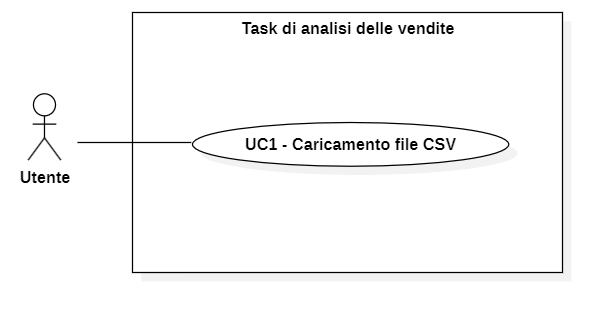
\includegraphics[width=0.9\columnwidth]{usecase/UC1 - Caricamento file CSV.png}
    \caption{UC1 - Caricamento file CSV}
\end{figure}

\usecaseactors{Utente}
\usecasepre{L'utente ha avviato la task di analisi delle vendite}
\usecasedesc{L'utente carica un file CSV contenente i dati delle vendite}
\usecasepost{Il sistema ha caricato il file CSV e lo ha memorizzato in un bucket del Google Cloud Storage}
\label{uc:caricamento-file-csv}
\end{usecase}


\hypertarget{UC2}{}
\begin{usecase}{2}{Selezione lingua per il report}

\begin{figure}[!h] 
    \centering 
    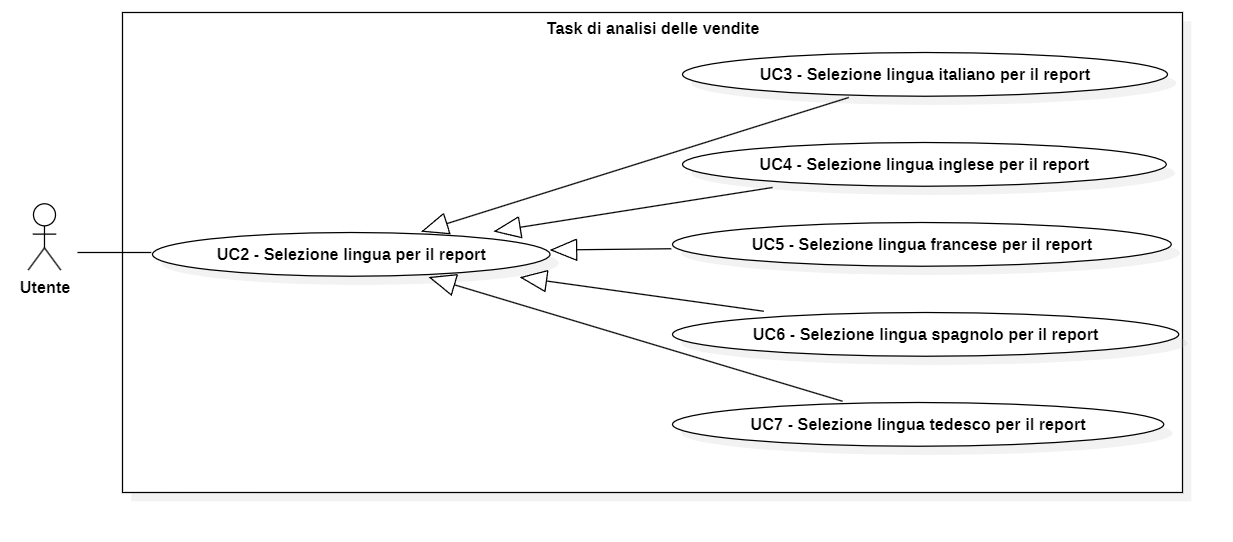
\includegraphics[width=0.9\columnwidth]{usecase/UC2 - Selezione lingua per il report.png}
    \caption{UC2 - Selezione lingua per il report}
\end{figure}

\usecaseactors{Utente}
\usecasepre{L'utente ha avviato la task di analisi delle vendite}
\usecasedesc{L'utente seleziona la lingua in cui desidera generare il report}
\usecasepost{Il sistema ha memorizzato la lingua selezionata}
\usespecial{UC3, UC4, UC5, UC6, UC7}
\label{uc:selezione-lingua-report}
\end{usecase}


\hypertarget{UC3}{}
\begin{usecase}{3}{Selezione lingua italiano per il report}

\usecaseactors{Utente}
\usecasepre{L'utente ha avviato la task di analisi delle vendite}
\usecasedesc{L'utente seleziona la lingua italiano perchè desidera generare il report in italiano}
\usecasepost{Il sistema ha memorizzato la lingua italiano selezionata}
\label{uc:selezione-lingua-italiano-report}
\end{usecase}


\hypertarget{UC4}{}
\begin{usecase}{4}{Selezione lingua inglese per il report}

\usecaseactors{Utente}
\usecasepre{L'utente ha avviato la task di analisi delle vendite}
\usecasedesc{L'utente seleziona la lingua inglese perchè desidera generare il report in inglese}
\usecasepost{Il sistema ha memorizzato la lingua inglese selezionata}
\label{uc:selezione-lingua-inglese-report}
\end{usecase}


\hypertarget{UC5}{}
\begin{usecase}{5}{Selezione lingua francese per il report}

\usecaseactors{Utente}
\usecasepre{L'utente ha avviato la task di analisi delle vendite}
\usecasedesc{L'utente seleziona la lingua francese perchè desidera generare il report in francese}
\usecasepost{Il sistema ha memorizzato la lingua francese selezionata}
\label{uc:selezione-lingua-francese-report}
\end{usecase}


\hypertarget{UC6}{}
\begin{usecase}{6}{Selezione lingua spagnolo per il report}

\usecaseactors{Utente}
\usecasepre{L'utente ha avviato la task di analisi delle vendite}
\usecasedesc{L'utente seleziona la lingua spagnolo perchè desidera generare il report in spagnolo}
\usecasepost{Il sistema ha memorizzato la lingua spagnolo selezionata}
\label{uc:selezione-lingua-spagnolo-report}
\end{usecase}


\hypertarget{UC7}{}
\begin{usecase}{7}{Selezione lingua tedesco per il report}

\usecaseactors{Utente}
\usecasepre{L'utente ha avviato la task di analisi delle vendite}
\usecasedesc{L'utente seleziona la lingua tedesco perchè desidera generare il report in tedesco}
\usecasepost{Il sistema ha memorizzato la lingua tedesco selezionata}
\label{uc:selezione-lingua-tedesco-report}
\end{usecase}


\hypertarget{UC8}{}
\begin{usecase}{8}{Selezione valuta per il report}

\begin{figure}[!h] 
    \centering 
    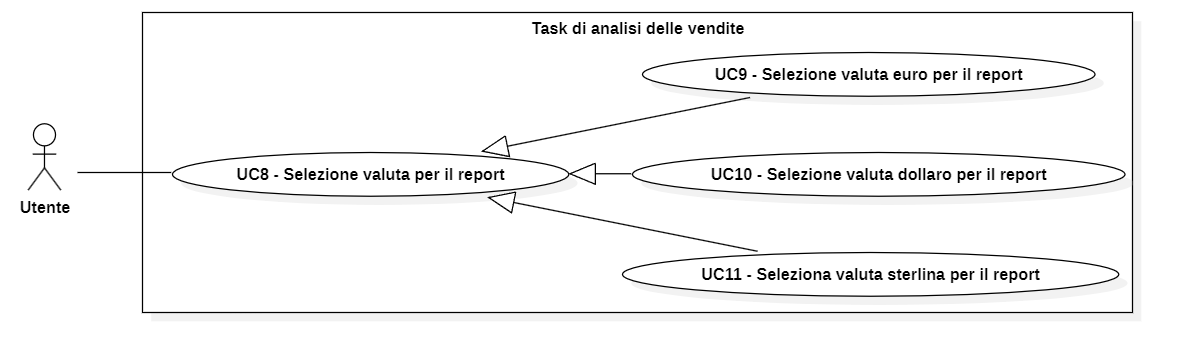
\includegraphics[width=0.9\columnwidth]{usecase/UC8 - Selezione valuta per il report.png}
    \caption{UC8 - Selezione valuta per il report}
\end{figure}

\usecaseactors{Utente}
\usecasepre{L'utente ha avviato la task di analisi delle vendite}
\usecasedesc{L'utente seleziona la valuta in cui desidera generare il report}
\usecasepost{Il sistema ha memorizzato la valuta selezionata}
\usespecial{UC9, UC10, UC11}
\label{uc:selezione-valuta-report}
\end{usecase}


\hypertarget{UC9}{}
\begin{usecase}{9}{Selezione valuta euro per il report}

\usecaseactors{Utente}
\usecasepre{L'utente ha avviato la task di analisi delle vendite}
\usecasedesc{L'utente seleziona la valuta euro perchè desidera generare il report con i valori monetari espressi in euro}
\usecasepost{Il sistema ha memorizzato la valuta euro selezionata}
\label{uc:selezione-valuta-euro-report}
\end{usecase}


\hypertarget{UC10}{}
\begin{usecase}{10}{Selezione valuta dollaro per il report}

\usecaseactors{Utente}
\usecasepre{L'utente ha avviato la task di analisi delle vendite}
\usecasedesc{L'utente seleziona la valuta dollaro perchè desidera generare il report con i valori monetari espressi in dollari}
\usecasepost{Il sistema ha memorizzato la valuta dollaro selezionata}
\label{uc:selezione-valuta-dollaro-report}
\end{usecase}


\hypertarget{UC11}{}
\begin{usecase}{11}{Selezione valuta sterlina per il report}

\usecaseactors{Utente}
\usecasepre{L'utente ha avviato la task di analisi delle vendite}
\usecasedesc{L'utente seleziona la valuta sterlina perchè desidera generare il report con i valori monetari espressi in sterline}
\usecasepost{Il sistema ha memorizzato la valuta sterlina selezionata}
\label{uc:selezione-valuta-sterlina-report}
\end{usecase}


\hypertarget{UC12}{}
\begin{usecase}{12}{Inserimento indirizzo email a cui inviare il report}

\begin{figure}[!h]
    \centering 
    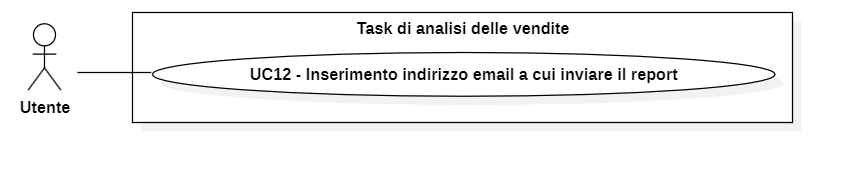
\includegraphics[width=0.9\columnwidth]{usecase/UC12 - Inserimento indirizzo email a cui inviare il report.png}
    \caption{UC12 - Inserimento indirizzo email a cui inviare il report}
\end{figure}

\usecaseactors{Utente}
\usecasepre{L'utente ha avviato la task di analisi delle vendite}
\usecasedesc{L'utente inserisce l'indirizzo email a cui desidera che venga inviato il report generato}
\usecasepost{Il sistema ha memorizzato l'indirizzo email inserito}

\end{usecase}


\hypertarget{UC13}{}
\begin{usecase}{13}{Visualizzazione esito positivo della task}

\begin{figure}[!h]
    \centering 
    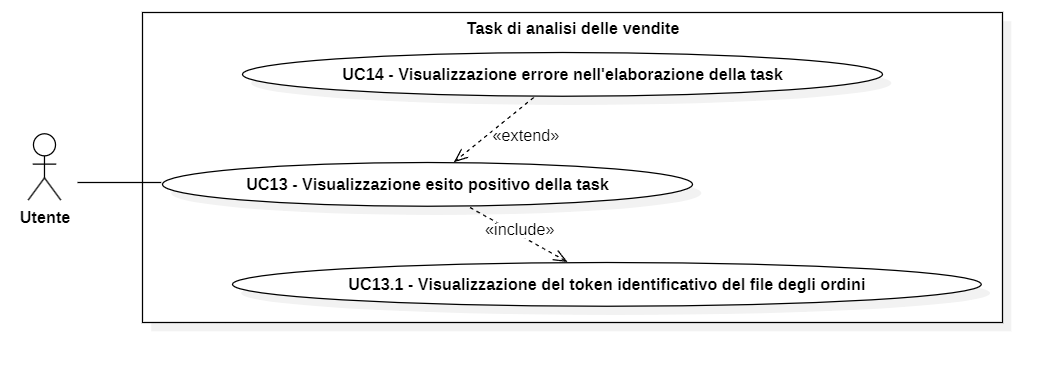
\includegraphics[width=0.9\columnwidth]{usecase/UC13 - Visualizzazione esito positivo della task.png}
    \caption{UC13 - Visualizzazione esito positivo della task}
\end{figure}

\usecaseactors{Utente}
\usecasepre{L'utente ha cliccato sul pulsante di esecuzione della task di analisi delle vendite}
\usecasedesc{L'utente visualizza l'esito positivo della task di analisi delle vendite}
\usecasepost{L'utente ha visualizzato l'esito positivo della task di analisi delle vendite}
\usecasealt{UC14}
\label{uc:visualizzazione-esito-positivo-task}
\end{usecase}


\hypertarget{UC13.1}{}
\begin{usecase}{13.1}{Visualizzazione del token identificativo del file degli ordini}

\usecaseactors{Utente}
\usecasepre{L'utente ha cliccato sul pulsante di esecuzione della task di analisi delle vendite}
\usecasedesc{L'utente visualizza il token identificativo del file degli ordini caricato}
\usecasepost{L'utente ha visualizzato il token identificativo del file degli ordini caricato}
\label{uc:visualizzazione-token-file-ordini}
\end{usecase}


\hypertarget{UC14}{}
\begin{usecase}{14}{Visualizzazione errore nell'elaborazione della task}

\usecaseactors{Utente}
\usecasepre{L'utente ha cliccato sul pulsante di esecuzione della task di analisi delle vendite}
\usecasedesc{L'utente visualizza un errore nell'elaborazione della task di analisi delle vendite}
\usecasepost{L'utente ha visualizzato un errore nell'elaborazione della task di analisi delle vendite}
\label{uc:visualizzazione-errore-task}
\end{usecase}


\hypertarget{UC15}{}
\begin{usecase}{15}{Download report delle vendite}

\begin{figure}[!h] 
    \centering 
    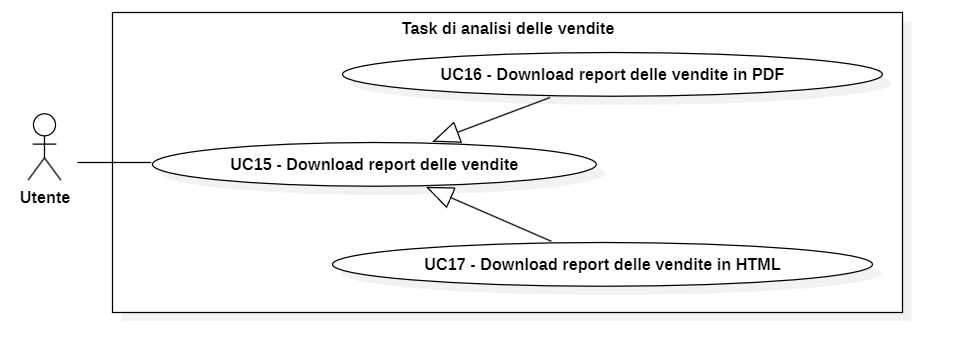
\includegraphics[width=0.9\columnwidth]{usecase/UC15 - Download report delle vendite.png}
    \caption{UC15 - Download report delle vendite}
\end{figure}

\usecaseactors{Utente}
\usecasepre{L'utente ha cliccato sul pulsante di esecuzione della task di analisi delle vendite}
\usecasedesc{L'utente scarica il report delle vendite generato dalla task di analisi delle vendite}
\usecasepost{L'utente ha scaricato il report delle vendite generato dalla task di analisi delle vendite}
\usespecial{UC16, UC17}
\label{uc:download-report-vendite}
\end{usecase}


\hypertarget{UC16}{}
\begin{usecase}{16}{Download report delle vendite in PDF}

\usecaseactors{Utente}
\usecasepre{L'utente ha cliccato sul pulsante di esecuzione della task di analisi delle vendite}
\usecasedesc{L'utente scarica il report delle vendite generato dalla task di analisi delle vendite in formato PDF}
\usecasepost{L'utente ha scaricato il report delle vendite generato dalla task di analisi delle vendite in formato PDF}
\label{uc:download-report-vendite-pdf}
\end{usecase}


\hypertarget{UC17}{}
\begin{usecase}{17}{Download report delle vendite in HTML}

\usecaseactors{Utente}
\usecasepre{L'utente ha cliccato sul pulsante di esecuzione della task di analisi delle vendite}
\usecasedesc{L'utente scarica il report delle vendite generato dalla task di analisi delle vendite in formato HTML}
\usecasepost{L'utente ha scaricato il report delle vendite generato dalla task di analisi delle vendite in formato HTML}
\label{uc:download-report-vendite-html}
\end{usecase}


\hypertarget{UC18}{}
\begin{usecase}{18}{Visualizzazione di un'email contenente il report delle vendite}

\begin{figure}[!h] 
    \centering 
    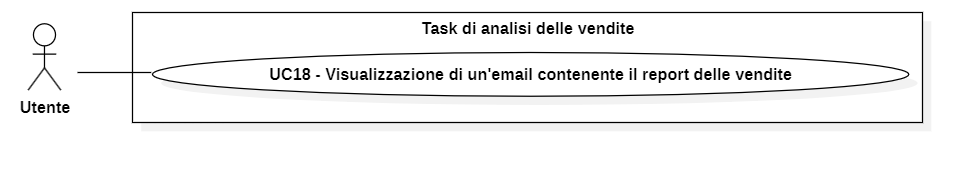
\includegraphics[width=0.9\columnwidth]{usecase/UC18 - Visualizzazione di un'email contenente il report delle vendite.png}
    \caption{UC18 - Visualizzazione di un'email contenente il report delle vendite}
\end{figure}

\usecaseactors{Utente}
\usecasepre{L'utente ha cliccato sul pulsante di esecuzione della task di analisi delle vendite, e poi ha visitato la propria casella di posta elettronica e cliccato sull'email ricevuta contenente il report delle vendite}
\usecasedesc{L'utente visualizza un'email contenente il report delle vendite generato dalla task di analisi delle vendite}
\usecasepost{L'utente ha visualizzato un'email contenente il report delle vendite generato dalla task di analisi delle vendite}
\useinclu{UC18.1, UC18.2, UC18.3}
\label{uc:visualizzazione-email-report-vendite}
\end{usecase}


\hypertarget{UC18.1}{}
\begin{usecase}{18.1}{Visualizzazione dati numerici}

\begin{figure}[!h] 
    \centering 
    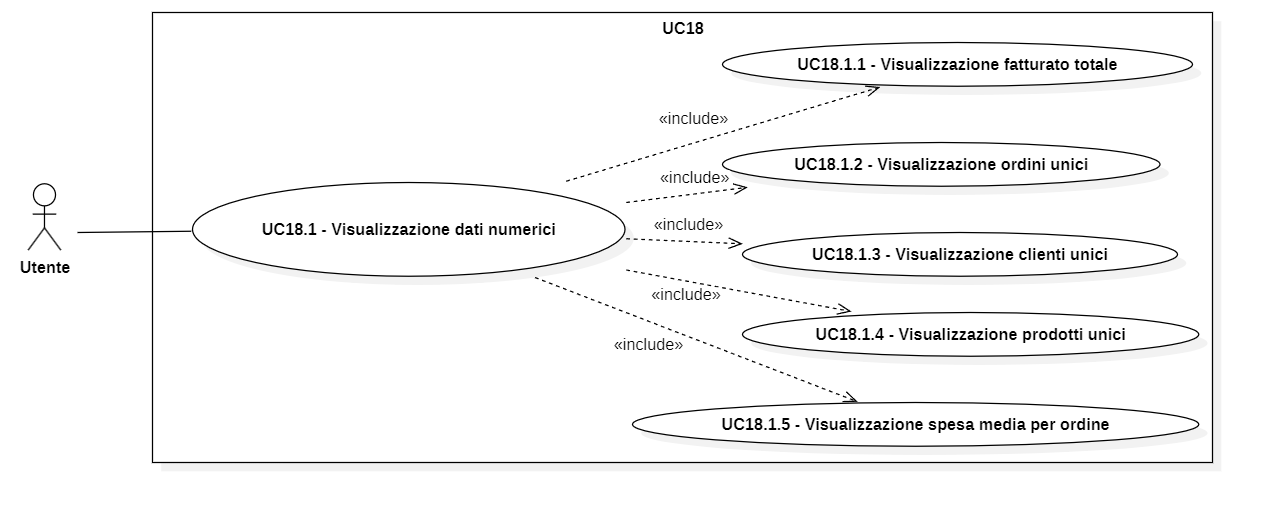
\includegraphics[width=0.9\columnwidth]{usecase/UC18.1 - Visualizzazione dati numerici.png}
    \caption{UC18.1 - Visualizzazione dati numerici}
\end{figure}

\usecaseactors{Utente}
\usecasepre{L'utente ha cliccato sul pulsante di esecuzione della task di analisi delle vendite, e poi ha visitato la propria casella di posta elettronica e cliccato sull'email ricevuta contenente il report delle vendite}
\usecasedesc{L'utente visualizza i dati numerici contenuti nel report delle vendite generato dalla task di analisi delle vendite}
\usecasepost{L'utente ha visualizzato i dati numerici contenuti nel report delle vendite generato dalla task di analisi delle vendite}
\useinclu{18.1.1, 18.1.2, 18.1.3, 18.1.4, 18.1.5}
\label{uc:visualizzazione-dati-numerici}
\end{usecase}


\hypertarget{UC18.1.1}{}
\begin{usecase}{18.1.1}{Visualizzazione fatturato totale}

\usecaseactors{Utente}
\usecasepre{L'utente ha cliccato sul pulsante di esecuzione della task di analisi delle vendite, e poi ha visitato la propria casella di posta elettronica e cliccato sull'email ricevuta contenente il report delle vendite}
\usecasedesc{L'utente visualizza il fatturato totale contenuto nel report delle vendite generato dalla task di analisi delle vendite}
\usecasepost{L'utente ha visualizzato il fatturato totale contenuto nel report delle vendite generato dalla task di analisi delle vendite}
\label{uc:visualizzazione-fatturato-totale}
\end{usecase}


\hypertarget{UC18.1.2}{}
\begin{usecase}{18.1.2}{Visualizzazione ordini unici}

\usecaseactors{Utente}
\usecasepre{L'utente ha cliccato sul pulsante di esecuzione della task di analisi delle vendite, e poi ha visitato la propria casella di posta elettronica e cliccato sull'email ricevuta contenente il report delle vendite}
\usecasedesc{L'utente visualizza il numero di ordini unici contenuti nel report delle vendite generato dalla task di analisi delle vendite}
\usecasepost{L'utente ha visualizzato il numero di ordini unici contenuti nel report delle vendite generato dalla task di analisi delle vendite}
\label{uc:visualizzazione-ordini-unici}
\end{usecase}


\hypertarget{UC18.1.3}{}
\begin{usecase}{18.1.3}{Visualizzazione clienti unici}

\usecaseactors{Utente}
\usecasepre{L'utente ha cliccato sul pulsante di esecuzione della task di analisi delle vendite, e poi ha visitato la propria casella di posta elettronica e cliccato sull'email ricevuta contenente il report delle vendite}
\usecasedesc{L'utente visualizza il numero di clienti unici contenuti nel report delle vendite generato dalla task di analisi delle vendite}
\usecasepost{L'utente ha visualizzato il numero di clienti unici contenuti nel report delle vendite generato dalla task di analisi delle vendite}
\label{uc:visualizzazione-clienti-unici}
\end{usecase}


\hypertarget{UC18.1.4}{}
\begin{usecase}{18.1.4}{Visualizzazione prodotti unici}

\usecaseactors{Utente}
\usecasepre{L'utente ha cliccato sul pulsante di esecuzione della task di analisi delle vendite, e poi ha visitato la propria casella di posta elettronica e cliccato sull'email ricevuta contenente il report delle vendite}
\usecasedesc{L'utente visualizza il numero di prodotti unici contenuti nel report delle vendite generato dalla task di analisi delle vendite}
\usecasepost{L'utente ha visualizzato il numero di prodotti unici contenuti nel report delle vendite generato dalla task di analisi delle vendite}
\label{uc:visualizzazione-prodotti-unici}
\end{usecase}


\hypertarget{UC18.1.5}{}
\begin{usecase}{18.1.5}{Visualizzazione spesa media per ordine}

\usecaseactors{Utente}
\usecasepre{L'utente ha cliccato sul pulsante di esecuzione della task di analisi delle vendite, e poi ha visitato la propria casella di posta elettronica e cliccato sull'email ricevuta contenente il report delle vendite}
\usecasedesc{L'utente visualizza la spesa media per ordine contenuta nel report delle vendite generato dalla task di analisi delle vendite}
\usecasepost{L'utente ha visualizzato la spesa media per ordine contenuta nel report delle vendite generato dalla task di analisi delle vendite}
\label{uc:visualizzazione-spesa-media-per-ordine}
\end{usecase}


\hypertarget{UC18.2}{}
\begin{usecase}{18.2}{Visualizzazione lista di grafici}

\begin{figure}[!h] 
    \centering 
    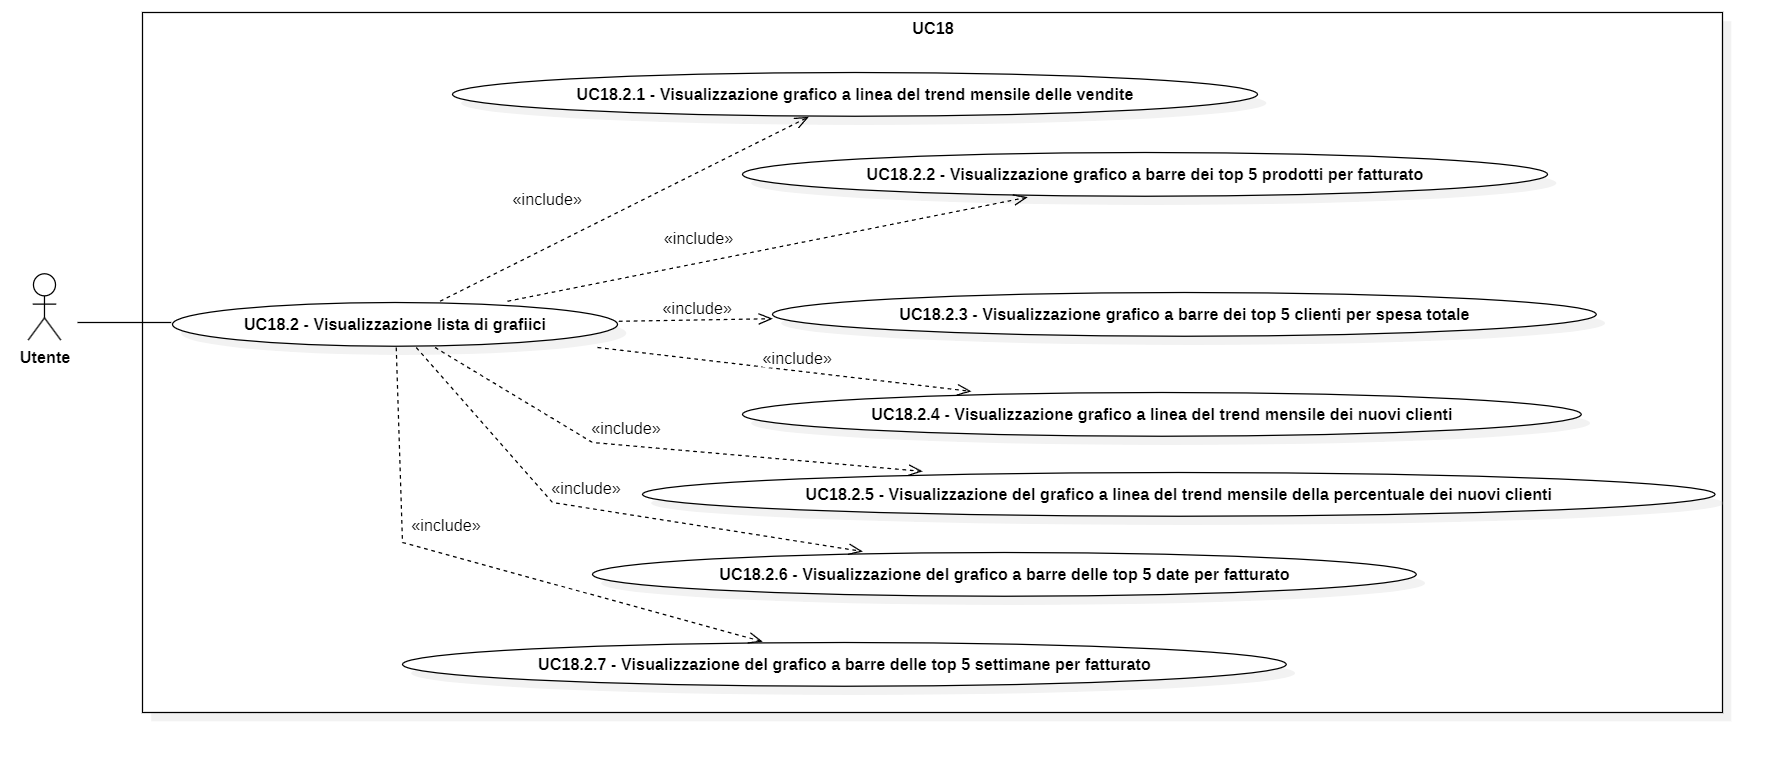
\includegraphics[width=0.9\columnwidth]{usecase/UC18.2 - Visualizzazione lista di grafici.png}
    \caption{UC18.2 - Visualizzazione lista di grafici}
\end{figure}

\usecaseactors{Utente}
\usecasepre{L'utente ha cliccato sul pulsante di esecuzione della task di analisi delle vendite, e poi ha visitato la propria casella di posta elettronica e cliccato sull'email ricevuta contenente il report delle vendite}
\usecasedesc{L'utente visualizza la lista di grafici contenuti nel report delle vendite generato dalla task di analisi delle vendite}
\usecasepost{L'utente ha visualizzato la lista di grafici contenuti nel report delle vendite generato dalla task di analisi delle vendite}
\useinclu{18.2.1, 18.2.2, 18.2.3, 18.2.4, 18.2.5, 18.2.6, 18.2.7}
\label{uc:visualizzazione-lista-grafici}
\end{usecase}


\hypertarget{UC18.2.1}{}
\begin{usecase}{18.2.1}{Visualizzazione grafico a linea del trend mensile delle vendite}

\usecaseactors{Utente}
\usecasepre{L'utente ha cliccato sul pulsante di esecuzione della task di analisi delle vendite, e poi ha visitato la propria casella di posta elettronica e cliccato sull'email ricevuta contenente il report delle vendite}
\usecasedesc{L'utente visualizza il grafico a linea del trend mensile delle vendite contenuto nel report delle vendite generato dalla task di analisi delle vendite}
\usecasepost{L'utente ha visualizzato il grafico a linea del trend mensile delle vendite contenuto nel report delle vendite generato dalla task di analisi delle vendite}
\label{uc:visualizzazione-grafico-trend-mensile-vendite}
\end{usecase}


\hypertarget{UC18.2.2}{}
\begin{usecase}{18.2.2}{Visualizzazione grafico a barre dei top 5 prodotti per fatturato}

\usecaseactors{Utente}
\usecasepre{L'utente ha cliccato sul pulsante di esecuzione della task di analisi delle vendite, e poi ha visitato la propria casella di posta elettronica e cliccato sull'email ricevuta contenente il report delle vendite}
\usecasedesc{L'utente visualizza il grafico a barre dei top 5 prodotti per fatturato contenuto nel report delle vendite generato dalla task di analisi delle vendite}
\usecasepost{L'utente ha visualizzato il grafico a barre dei top 5 prodotti per fatturato contenuto nel report delle vendite generato dalla task di analisi delle vendite}
\label{uc:visualizzazione-grafico-top-5-prodotti-fatturato}
\end{usecase}


\hypertarget{UC18.2.3}{}
\begin{usecase}{18.2.3}{Visualizzazione grafico a barre dei top 5 clienti per spesa totale}

\usecaseactors{Utente}
\usecasepre{L'utente ha cliccato sul pulsante di esecuzione della task di analisi delle vendite, e poi ha visitato la propria casella di posta elettronica e cliccato sull'email ricevuta contenente il report delle vendite}
\usecasedesc{L'utente visualizza il grafico a barre dei top 5 clienti per spesa totale contenuto nel report delle vendite generato dalla task di analisi delle vendite}
\usecasepost{L'utente ha visualizzato il grafico a barre dei top 5 clienti per spesa totale contenuto nel report delle vendite generato dalla task di analisi delle vendite}
\label{uc:visualizzazione-grafico-top-5-clienti-spesa-totale}
\end{usecase}


\hypertarget{UC18.2.4}{}
\begin{usecase}{18.2.4}{Visualizzazione grafico a linea del trend mensile dei nuovi clienti}

\usecaseactors{Utente}
\usecasepre{L'utente ha cliccato sul pulsante di esecuzione della task di analisi delle vendite, e poi ha visitato la propria casella di posta elettronica e cliccato sull'email ricevuta contenente il report delle vendite}
\usecasedesc{L'utente visualizza il grafico a linea del trend mensile dei nuovi clienti contenuto nel report delle vendite generato dalla task di analisi delle vendite}
\usecasepost{L'utente ha visualizzato il grafico a linea del trend mensile dei nuovi clienti contenuto nel report delle vendite generato dalla task di analisi delle vendite}
\label{uc:visualizzazione-grafico-trend-mensile-nuovi-clienti}
\end{usecase}


\hypertarget{UC18.2.5}{}
\begin{usecase}{18.2.5}{Visualizzazione del grafico a linea del trend mensile della percentuale dei nuovi clienti}

\usecaseactors{Utente}
\usecasepre{L'utente ha cliccato sul pulsante di esecuzione della task di analisi delle vendite, e poi ha visitato la propria casella di posta elettronica e cliccato sull'email ricevuta contenente il report delle vendite}
\usecasedesc{L'utente visualizza il grafico a linea del trend mensile della percentuale dei nuovi clienti contenuto nel report delle vendite generato dalla task di analisi delle vendite}
\usecasepost{L'utente ha visualizzato il grafico a linea del trend mensile della percentuale dei nuovi clienti contenuto nel report delle vendite generato dalla task di analisi delle vendite}
\label{uc:visualizzazione-grafico-trend-mensile-percentuale-nuovi-clienti}
\end{usecase}


\hypertarget{UC18.2.6}{}
\begin{usecase}{18.2.6}{Visualizzazione del grafico a barre delle top 5 date per fatturato}

\usecaseactors{Utente}
\usecasepre{L'utente ha cliccato sul pulsante di esecuzione della task di analisi delle vendite, e poi ha visitato la propria casella di posta elettronica e cliccato sull'email ricevuta contenente il report delle vendite}
\usecasedesc{L'utente visualizza il grafico a barre delle top 5 date per fatturato contenuto nel report delle vendite generato dalla task di analisi delle vendite}
\usecasepost{L'utente ha visualizzato il grafico a barre delle top 5 date per fatturato contenuto nel report delle vendite generato dalla task di analisi delle vendite}
\label{uc:visualizzazione-grafico-top-5-date-fatturato}
\end{usecase}


\hypertarget{UC18.2.7}{}
\begin{usecase}{18.2.7}{Visualizzazione del grafico a barre delle top 5 settimane per fatturato}

\usecaseactors{Utente}
\usecasepre{L'utente ha cliccato sul pulsante di esecuzione della task di analisi delle vendite, e poi ha visitato la propria casella di posta elettronica e cliccato sull'email ricevuta contenente il report delle vendite}
\usecasedesc{L'utente visualizza il grafico a barre delle top 5 settimane per fatturato contenuto nel report delle vendite generato dalla task di analisi delle vendite}
\usecasepost{L'utente ha visualizzato il grafico a barre delle top 5 settimane per fatturato contenuto nel report delle vendite generato dalla task di analisi delle vendite}
\label{uc:visualizzazione-grafico-top-5-settimane-fatturato}
\end{usecase}


\hypertarget{UC18.3}{}
\begin{usecase}{18.3}{Visualizzazione resoconto dell'analisi delle vendite}

\begin{figure}[!h] 
    \centering 
    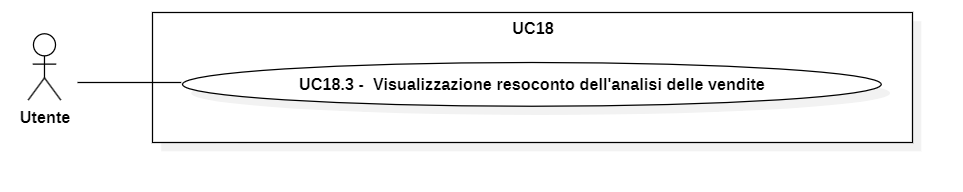
\includegraphics[width=0.9\columnwidth]{usecase/UC18.3 - Visualizzazione resoconto dell'analisi delle vendite.png}
    \caption{UC18.3 - Visualizzazione resoconto dell'analisi delle vendite}
\end{figure}

\usecaseactors{Utente}
\usecasepre{L'utente ha cliccato sul pulsante di esecuzione della task di analisi delle vendite, e poi ha visitato la propria casella di posta elettronica e cliccato sull'email ricevuta contenente il report delle vendite}
\usecasedesc{L'utente visualizza il resoconto dell'analisi delle vendite contenuto nel report delle vendite generato dalla task di analisi delle vendite}
\usecasepost{L'utente ha visualizzato il resoconto dell'analisi delle vendite contenuto nel report delle vendite generato dalla task di analisi delle vendite}
\label{uc:visualizzazione-resoconto-analisi-vendite}
\end{usecase}


\hypertarget{UC18.4}{}
\begin{usecase}{18.4}{Visualizzazione del token identificativo del file degli ordini}

\begin{figure}[!h] 
    \centering 
    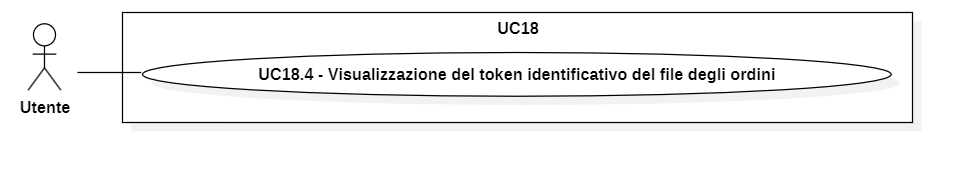
\includegraphics[width=0.9\columnwidth]{usecase/UC18.4 - Visualizzazione del token identificativo del file degli ordini.png}
    \caption{UC18.4 - Visualizzazione del token identificativo del file degli ordini}
\end{figure}

\usecaseactors{Utente}
\usecasepre{L'utente ha cliccato sul pulsante di esecuzione della task di analisi delle vendite, e poi ha visitato la propria casella di posta elettronica e cliccato sull'email ricevuta contenente il report delle vendite}
\usecasedesc{L'utente visualizza il token identificativo del file degli ordini caricato}
\usecasepost{L'utente ha visualizzato il token identificativo del file degli ordini caricato}
\label{uc:visualizzazione-token-file-ordini-mail}
\end{usecase}


\hypertarget{UC19}{}
\begin{usecase}{19}{Inserimento del token identificativo del file degli ordini}

\begin{figure}[!h] 
    \centering 
    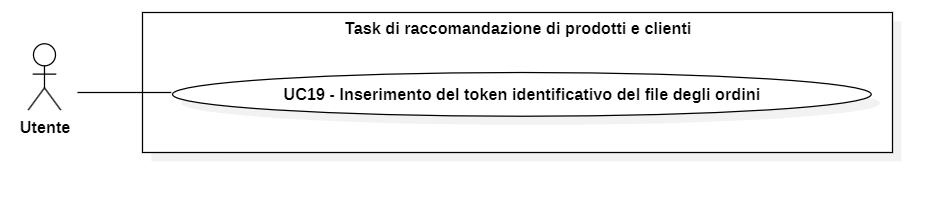
\includegraphics[width=0.9\columnwidth]{usecase/UC19 - Inserimento del token identificativo del file degli ordini.png}
    \caption{UC19 - Inserimento del token identificativo del file degli ordini}
\end{figure}

\usecaseactors{Utente}
\usecasepre{L'utente ha eseguito con successo la task di analisi delle vendite e poi ha avviato la task di raccomandazione di prodotti e clienti}
\usecasedesc{L'utente inserisce il token identificativo del file degli ordini, che era stato generato dalla task di analisi delle vendite}
\usecasepost{Il sistema ricerca il bucket corrispondente al token identificativo all'interno del Google Cloud Storage}
\label{uc:inserimento-nome-file-csv}
\end{usecase}


\hypertarget{UC20}{}
\begin{usecase}{20}{Selezione tipo di raccomandazione}

\begin{figure}[!h] 
    \centering 
    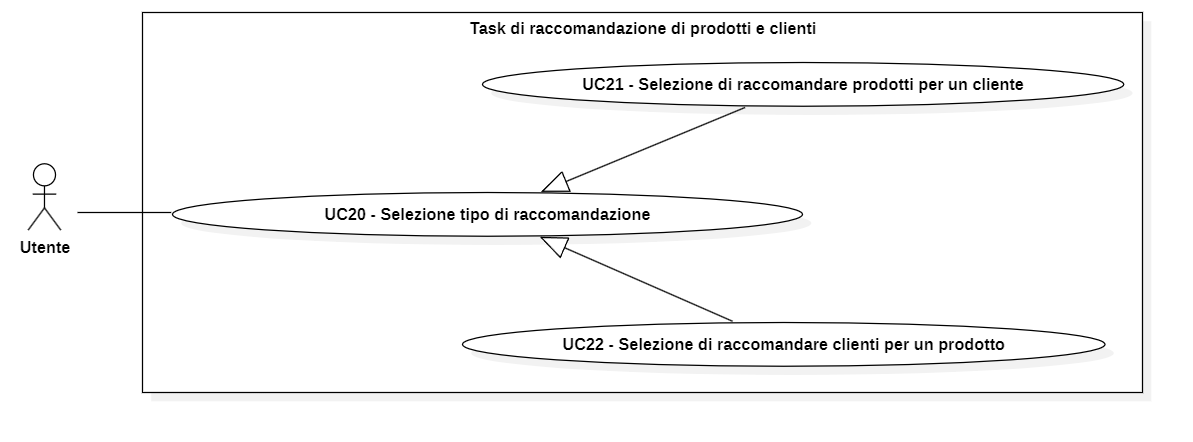
\includegraphics[width=0.9\columnwidth]{usecase/UC20 - Selezione tipo di raccomandazione.png}
    \caption{UC20 - Selezione tipo di raccomandazione}
\end{figure}

\usecaseactors{Utente}
\usecasepre{L'utente ha eseguito con successo la task di analisi delle vendite e poi ha avviato la task di raccomandazione di prodotti e clienti}
\usecasedesc{L'utente seleziona la tipologia di raccomandazione che desidera che venga eseguita, tra le seguenti: "Raccomandare prodotti per un cliente" o "Raccomandare clienti per un prodotto"}
\usecasepost{Il sistema ha memorizzato il tipo di raccomandazione selezionato}
\usespecial{UC21, UC22}
\label{uc:selezione-tipo-elemento}
\end{usecase}


\hypertarget{UC21}{}
\begin{usecase}{21}{Selezione di raccomandare prodotti per un cliente}

\usecaseactors{Utente}
\usecasepre{L'utente ha eseguito con successo la task di analisi delle vendite e poi ha avviato la task di raccomandazione di prodotti e clienti}
\usecasedesc{L'utente seleziona il tipo di raccomandazione "Raccomandare prodotti per un cliente"}
\usecasepost{Il sistema ha memorizzato il tipo di raccomandazione "Raccomandare prodotti per un cliente" selezionato}
\label{uc:selezione-raccomandare-prodotti}
\end{usecase}


\hypertarget{UC22}{}
\begin{usecase}{22}{Selezione di raccomandare clienti per un prodotto}

\usecaseactors{Utente}
\usecasepre{L'utente ha eseguito con successo la task di analisi delle vendite e poi ha avviato la task di raccomandazione di prodotti e clienti}
\usecasedesc{L'utente seleziona il tipo di raccomandazione "Raccomandare clienti per un prodotto"}
\usecasepost{Il sistema ha memorizzato il tipo di raccomandazione "Raccomandare clienti per un prodotto" selezionato}
\label{uc:selezione-raccomandare-clienti}
\end{usecase}


\hypertarget{UC23}{}
\begin{usecase}{23}{Inserimento nome elemento a cui raccomandare}

\begin{figure}[!h] 
    \centering 
    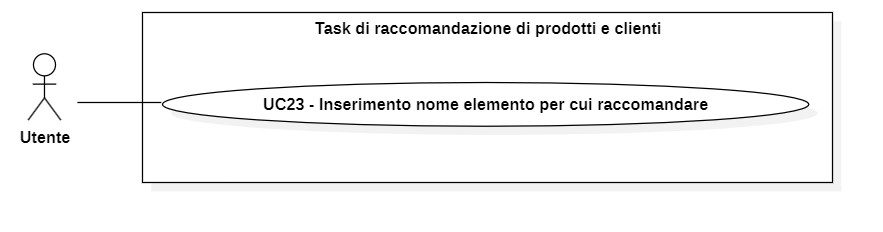
\includegraphics[width=0.9\columnwidth]{usecase/UC23 - Inserimento nome elemento a cui raccomandare.png}
    \caption{UC23 - Inserimento nome elemento a cui raccomandare}
\end{figure}

\usecaseactors{Utente}
\usecasepre{L'utente ha eseguito con successo la task di analisi delle vendite e poi ha avviato la task di raccomandazione di prodotti e clienti}
\usecasedesc{L'utente inserisce il nome dell'elemento a cui desidera che vengano raccomandati prodotti o clienti, a seconda del tipo di raccomandazione selezionato}
\usecasepost{Il sistema cerca l'elemento corrispondente al nome inserito all'interno del file salvato nel Google Cloud Storage}
\label{uc:inserimento-nome-elemento}
\end{usecase}


\hypertarget{UC24}{}
\begin{usecase}{24}{Inserimento del numero di raccomandazioni desiderate}

\begin{figure}[!h] 
    \centering 
    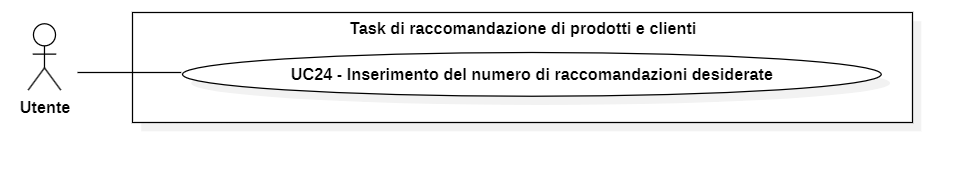
\includegraphics[width=0.9\columnwidth]{usecase/UC24 - Inserimento del numero di raccomandazioni desiderate.png}
    \caption{UC24 - Inserimento del numero di raccomandazioni desiderate}
\end{figure}

\usecaseactors{Utente}
\usecasepre{L'utente ha eseguito con successo la task di analisi delle vendite e poi ha avviato la task di raccomandazione di prodotti e clienti}
\usecasedesc{L'utente inserisce il numero di raccomandazioni che desidera che vengano generate}
\usecasepost{Il sistema ha memorizzato il numero di raccomandazioni desiderate}
\label{uc:inserimento-numero-raccomandazioni}
\end{usecase}


\hypertarget{UC25}{}
\begin{usecase}{25}{Selezione lingua per la raccomandazione}

\begin{figure}[!h] 
    \centering 
    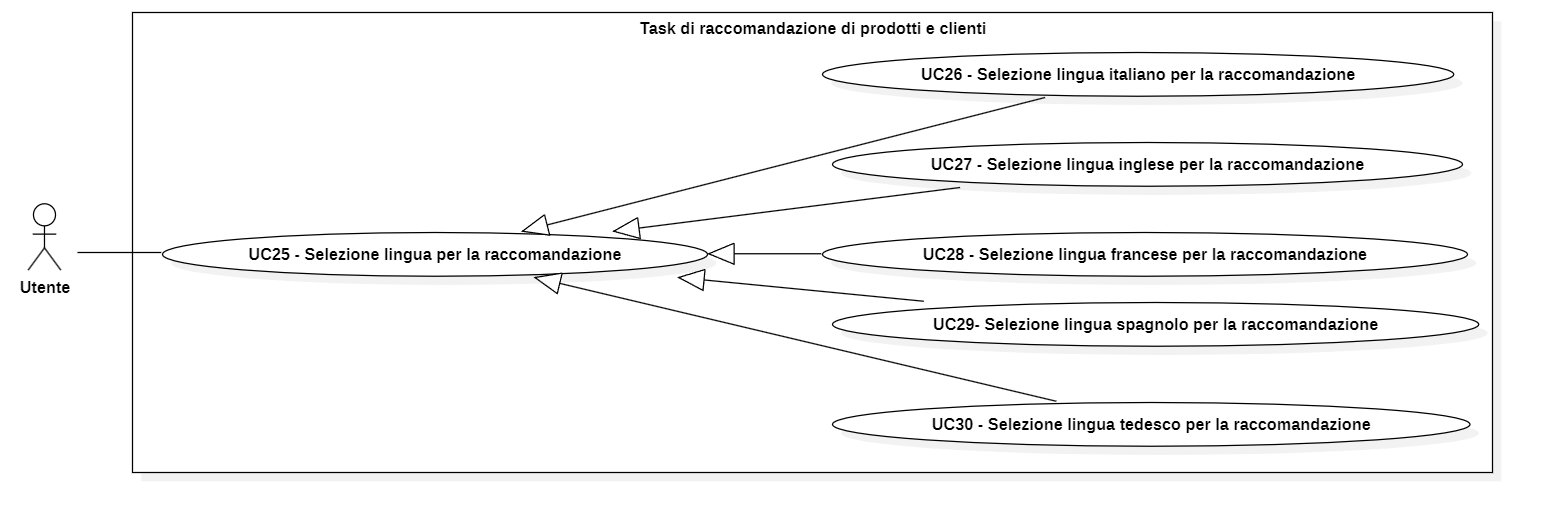
\includegraphics[width=0.9\columnwidth]{usecase/UC25 - Selezione lingua per la raccomandazione.png}
    \caption{UC25 - Selezione lingua per la raccomandazione}
\end{figure}

\usecaseactors{Utente}
\usecasepre{L'utente ha eseguito con successo la task di analisi delle vendite e poi ha avviato la task di raccomandazione di prodotti e clienti}
\usecasedesc{L'utente seleziona la lingua in cui desidera generare la raccomandazione}
\usecasepost{Il sistema ha memorizzato la lingua selezionata}
\usespecial{UC26, UC27, UC28, UC29, UC30}
\label{uc:selezione-lingua-raccomandazione}
\end{usecase}


\hypertarget{UC26}{}
\begin{usecase}{26}{Selezione lingua italiano per la raccomandazione}

\usecaseactors{Utente}
\usecasepre{L'utente ha eseguito con successo la task di analisi delle vendite e poi ha avviato la task di raccomandazione di prodotti e clienti}
\usecasedesc{L'utente seleziona la lingua italiano perchè desidera generare la raccomandazione in italiano}
\usecasepost{Il sistema ha memorizzato la lingua italiano selezionata}
\label{uc:selezione-lingua-italiano-raccomandazione}
\end{usecase}


\hypertarget{UC27}{}
\begin{usecase}{27}{Selezione lingua inglese per la raccomandazione}

\usecaseactors{Utente}
\usecasepre{L'utente ha eseguito con successo la task di analisi delle vendite e poi ha avviato la task di raccomandazione di prodotti e clienti}
\usecasedesc{L'utente seleziona la lingua inglese perchè desidera generare la raccomandazione in inglese}
\usecasepost{Il sistema ha memorizzato la lingua inglese selezionata}
\label{uc:selezione-lingua-inglese-raccomandazione}
\end{usecase}


\hypertarget{UC28}{}
\begin{usecase}{28}{Selezione lingua francese per la raccomandazione}

\usecaseactors{Utente}
\usecasepre{L'utente ha eseguito con successo la task di analisi delle vendite e poi ha avviato la task di raccomandazione di prodotti e clienti}
\usecasedesc{L'utente seleziona la lingua francese perchè desidera generare la raccomandazione in francese}
\usecasepost{Il sistema ha memorizzato la lingua francese selezionata}
\label{uc:selezione-lingua-francese-raccomandazione}
\end{usecase}


\hypertarget{UC29}{}
\begin{usecase}{29}{Selezione lingua spagnolo per la raccomandazione}

\usecaseactors{Utente}
\usecasepre{L'utente ha eseguito con successo la task di analisi delle vendite e poi ha avviato la task di raccomandazione di prodotti e clienti}
\usecasedesc{L'utente seleziona la lingua spagnolo perchè desidera generare la raccomandazione in spagnolo}
\usecasepost{Il sistema ha memorizzato la lingua spagnolo selezionata}
\label{uc:selezione-lingua-spagnolo-raccomandazione}
\end{usecase}


\hypertarget{UC30}{}
\begin{usecase}{30}{Selezione lingua tedesco per la raccomandazione}

\usecaseactors{Utente}
\usecasepre{L'utente ha eseguito con successo la task di analisi delle vendite e poi ha avviato la task di raccomandazione di prodotti e clienti}
\usecasedesc{L'utente seleziona la lingua tedesco perchè desidera generare la raccomandazione in tedesco}
\usecasepost{Il sistema ha memorizzato la lingua tedesco selezionata}
\label{uc:selezione-lingua-tedesco-raccomandazione}
\end{usecase}


\hypertarget{UC31}{}
\begin{usecase}{31}{Visualizzazione classifica elementi raccomandati}

\begin{figure}[!h]
    \centering 
    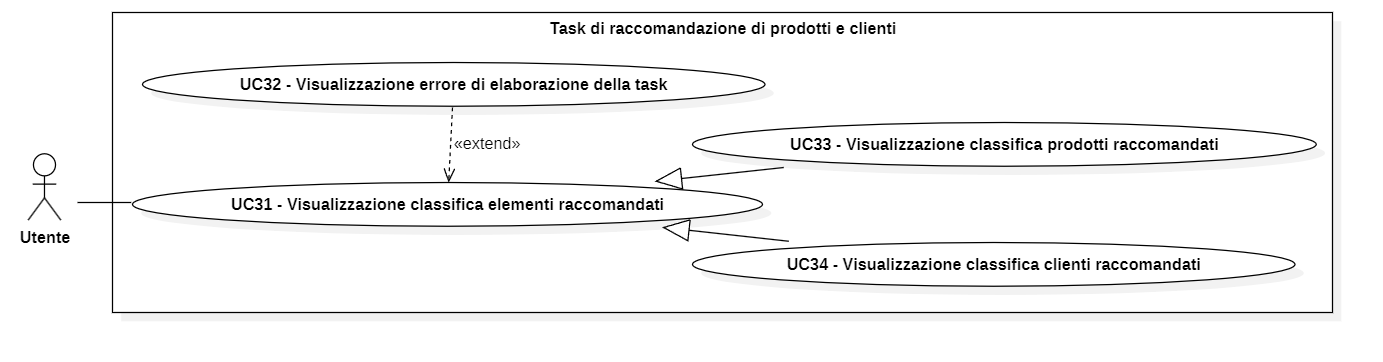
\includegraphics[width=0.9\columnwidth]{usecase/UC31 - Visualizzazione classifica elementi raccomandati.png}
    \caption{UC31 - Visualizzazione classifica elementi raccomandati}
\end{figure}

\usecaseactors{Utente}
\usecasepre{L'utente ha cliccato sul pulsante di esecuzione della task di raccomandazione di prodotti e clienti}
\usecasedesc{L'utente visualizza la classifica degli elementi raccomandati}
\usecasepost{L'utente ha visualizzato la classifica degli elementi raccomandati}
\usecasealt{UC32}
\usespecial{UC33, UC34}
\label{uc:visualizzazione-classifica-elementi-raccomandati}
\end{usecase}


\hypertarget{UC32}{}
\begin{usecase}{32}{Visualizzazione errore di elaborazione della task}

\usecaseactors{Utente}
\usecasepre{L'utente ha cliccato sul pulsante di esecuzione della task di raccomandazione di prodotti e clienti}
\usecasedesc{L'utente visualizza un errore nell'elaborazione della task di raccomandazione di prodotti e clienti}
\usecasepost{L'utente ha visualizzato un errore nell'elaborazione della task di raccomandazione di prodotti e clienti}
\label{uc:visualizzazione-errore-elaborazione-task}
\end{usecase}


\hypertarget{UC33}{}
\begin{usecase}{33}{Visualizzazione classifica prodotti raccomandati}

\usecaseactors{Utente}
\usecasepre{L'utente ha cliccato sul pulsante di esecuzione della task di raccomandazione di prodotti e clienti}
\usecasedesc{L'utente visualizza la classifica dei prodotti raccomandati}
\usecasepost{L'utente ha visualizzato la classifica dei prodotti raccomandati}
\label{uc:visualizzazione-classifica-prodotti-raccomandati}
\end{usecase}


\hypertarget{UC34}{}
\begin{usecase}{34}{Visualizzazione classifica clienti raccomandati}

\usecaseactors{Utente}
\usecasepre{L'utente ha cliccato sul pulsante di esecuzione della task di raccomandazione di prodotti e clienti}
\usecasedesc{L'utente visualizza la classifica dei clienti raccomandati}
\usecasepost{L'utente ha visualizzato la classifica dei clienti raccomandati}
\label{uc:visualizzazione-classifica-clienti-raccomandati}
\end{usecase}



\newpage









\section{Tracciamento dei requisiti}

Da un'attenta analisi dei requisiti e dei casi d'uso effettuata sul progetto è stata stilata la tabella che traccia i requisiti in rapporto ai casi d'uso.

Sono stati individuati diversi tipi di requisiti e si è quindi fatto utilizzo di un codice identificativo per distinguerli.

Il codice dei requisiti è così strutturato:
\begin{center}
    \textbf{R[importanza][tipo]-[numero]}
\end{center}
dove:
\begin{itemize}
	\item L'importanza può essere O per i requisiti obbligatori, D per quelli desiderabili oppure Z per quelli opzionali;
	\item Il tipo può essere F per i requisiti funzionali, Q per quelli qualitativi oppure V per quelli di vincolo;
	\item Il numero è un valore numerico progressivo che identifica univocamente un requisito.
\end{itemize}
Nelle tabelle \ref{tab:requisiti-funzionali}, \ref{tab:requisiti-qualitativi} e \ref{tab:requisiti-vincolo} sono riassunti, rispettivamente, i requisiti funzionali, qualitativi e di vincolo, e l’eventuale loro tracciamento con i casi d'uso delineati in fase di analisi.


\subsection{Requisiti funzionali}

\RequisitiTable
  {Tabella di tracciamento dei requisiti funzionali}
  {tab:requisiti-funzionali}
  {\textbf{Requisito} & \textbf{Descrizione} & \textbf{Fonti}}

ROF-1 & Il sistema deve permettere all'utente di caricare un file CSV contenente gli ordini. & \hyperlink{UC1}{UC1} \\ \hline
ROF-2 & Il sistema deve permettere all'utente di selezionare la lingua da usare per generare il report, tra italiano, inglese, francese, spagnolo e tedesco. & \hyperlink{UC2}{UC2}, \hyperlink{UC3}{UC3}, \hyperlink{UC4}{UC4}, \hyperlink{UC5}{UC5}, \hyperlink{UC6}{UC6} e \hyperlink{UC7}{UC7} \\ \hline
ROF-3 & Il sistema deve permettere all'utente di selezionare la valuta da usare per generare il report, tra euro, dollaro e sterlina. & \hyperlink{UC8}{UC8}, \hyperlink{UC9}{UC9}, \hyperlink{UC10}{UC10} e \hyperlink{UC11}{UC11} \\ \hline
ROF-4 & Il sistema deve permettere all'utente di inserire l'indirizzo email a cui inviare il report generato dalla task di analisi delle vendite. & \hyperlink{UC12}{UC12} \\ \hline
ROF-5 & Nel caso la task di analisi delle vendite sia stata eseguita correttamente, il sistema deve permettere all'utente di visualizzare l'esito positivo della task. & \hyperlink{UC13}{UC13} \\ \hline
ROF-6 & Nel caso la task di analisi delle vendite sia stata eseguita correttamente, il sistema deve permettere all'utente di visualizzare il token identificativo del bucket di Google Cloud Storage in cui è stato salvato il file degli ordini, e di copiarlo negli appunti. & Azienda, \hyperlink{UC13.1}{UC13.1} \\ \hline
ROF-7 & Nel caso avvenga un imprevisto, il sistema deve permettere all'utente di visualizzare un messaggio che segnala un errore di elaborazione della task. & \hyperlink{UC14}{UC14} \\ \hline
ROF-8 & Il sistema deve permettere all'utente di scaricare il report generato dalla task di analisi delle vendite, in formato PDF. & \hyperlink{UC15}{UC15}, \hyperlink{UC16}{UC16}\\ \hline
RDF-9 & Il sistema deve permettere all'utente di scaricare il report generato dalla task di analisi delle vendite, in formato HTML. & \hyperlink{UC15}{UC15}, \hyperlink{UC17}{UC17} \\ \hline
RZF-10 & Il sistema deve inviare il report generato dalla task di analisi delle vendite all'indirizzo email inserito dall'utente. Il testo della mail deve contenere l'HTML del report, e i file PDF e HTML devono essere inviati in allegato. & \hyperlink{UC18}{UC18} \\ \hline
ROF-11 & Nel report delle vendite generato, l'utente deve visualizzare alcuni dati numerici legati alle vendite. & Azienda, \hyperlink{18.1}, \hyperlink{UC18.1.1}{UC18.1.1}, \hyperlink{UC18.1.2}{UC18.1.2}, \hyperlink{UC18.1.3}{UC18.1.3}, \hyperlink{UC18.1.4}{UC18.1.4} e \hyperlink{UC18.1.5}{UC18.1.5} \\ \hline
ROF-12 & Nel report delle vendite generato, l'utente deve visualizzare alcuni grafici generati a partire dai dati delle vendite. & Azienda, \hyperlink{UC18.2}{UC18.2}, \hyperlink{UC18.2.1}{UC18.2.1}, \hyperlink{UC18.2.2}{UC18.2.2}, \hyperlink{UC18.2.3}{UC18.2.3}, \hyperlink{UC18.2.4}{UC18.2.4}, \hyperlink{UC18.2.5}{UC18.2.5}, \hyperlink{UC18.2.6}{UC18.2.6} e \hyperlink{UC18.2.7}{UC18.2.7} \\ \hline
ROF-13 & Nel report delle vendite generato, l'utente deve visualizzare un resoconto dell'analisi delle vendite, generato dall'LLM. & Azienda, \hyperlink{UC18.3}{UC18.3} \\ \hline
RZF-14 & Nella mail inviata all'utente, l'utente deve visualizzare il token identificativo del bucket di Google Cloud Storage in cui è stato salvato il file degli ordini, e deve poterlo copiare negli appunti. & Azienda, \hyperlink{UC18.4}{UC18.4} \\ \hline
ROF-15 & Il sistema deve permettere all'utente di inserire il token identificativo del bucket di Google Cloud Storage in cui è stato salvato il file degli ordini, il quale era stato generato e mostrato nella task di analisi delle vendite. & \hyperlink{UC19}{UC19} \\ \hline
ROF-16 & Il sistema deve permettere all'utente di selezionare il tipo di raccomandazione da svolgere, tra "Raccomandare prodotti per un cliente" e "Raccomandare clienti per un prodotto". & \hyperlink{UC20}{UC20}, \hyperlink{UC21}{UC21} e \hyperlink{UC22}{UC22} \\ \hline
ROF-17 & Il sistema deve permettere all'utente di inserire il nome dell'elemento a cui desidera che vengano raccomandati prodotti o clienti, a seconda del tipo di raccomandazione selezionato. & \hyperlink{UC23}{UC23} \\ \hline
ROF-18 & Il sistema deve permettere all'utente di inserire il numero di raccomandazioni che desidera che vengano generate. & \hyperlink{UC24}{UC24} \\ \hline
ROF-19 & Il sistema deve permettere all'utente di selezionare la lingua da usare per generare la raccomandazione, tra italiano, inglese, francese, spagnolo e tedesco. & \hyperlink{UC25}{UC25}, \hyperlink{UC26}{UC26}, \hyperlink{UC27}{UC27}, \hyperlink{UC28}{UC28}, \hyperlink{UC29}{UC29} e \hyperlink{UC30}{UC30} \\ \hline
ROF-20 & Nel caso la task di raccomandazione sia stata eseguita correttamente, il sistema deve permettere all'utente di visualizzare la classifica degli elementi raccomandati. & \hyperlink{UC31}{UC31}, \hyperlink{UC33}{UC33} e \hyperlink{UC34}{UC34} \\ \hline
ROF-21 & Nel caso avvenga un imprevisto, il sistema deve permettere all'utente di visualizzare un messaggio che segnala un errore di elaborazione della task. & \hyperlink{UC32}{UC32} \\ \hline

\end{longtable}


\subsection{Requisiti qualitativi}

\RequisitiTable
  {Tabella di tracciamento dei requisiti qualitativi}
  {tab:requisiti-qualitativi}
  {\textbf{Requisito} & \textbf{Descrizione} & \textbf{Fonti}}

ROQ-1 & Il lavoro svolto deve essere opportunamente documentato. & OO6 \\ \hline
ROQ-2 & Il codice prodotto deve essere completamente coperto da test di unità. & OO6 \\ \hline
ROQ-3 & Le risposte prodotte dall'LLM devono essere testate, dopo aver definito un opportuno metodo di test. & Azienda, OO6 \\ \hline
RDQ-4 & La task di raccomandazione di prodotti e clienti deve produrre un risultato in tempi ragionevoli. & Azienda, OD1 \\ \hline
RZQ-5 & Le raccomandazioni devono essere "Explainable", in modo che un tecnico aziendale possa comprendere il motivo per cui sono stati raccomandati determinati prodotti o clienti come output ad un utente. & OZ2 \\ \hline

\end{longtable}


\subsection{Requisiti di vincolo}

\RequisitiTable
  {Tabella di tracciamento dei requisiti di vincolo}
  {tab:requisiti-vincolo}
  {\textbf{Requisito} & \textbf{Descrizione} & \textbf{Fonti}}

ROV-1 & Le funzionalità devono essere espresse mediante due task create usando la piattaforma Oribea. & OO3, OO4 \\ \hline
ROV-2 & I due progetti software delle due tasks devono essere inseriti nel campo function della schermata di creazione task della piattaforma Oribea. & Azienda, OO1 \\ \hline
ROV-3 & I due progetti software delle due tasks devono essere caricati come due repository nel profilo GitHub dell'azienda Oribea. & Azienda \\ \hline
ROV-4 & Le due task devono utilizzare, come archiviazione, il profilo Google Cloud dell'azienda Oribea. & Azienda, OO2 \\ \hline
ROV-5 & La task di analisi delle vendite deve permettere il download del report in formato PDF. & Azienda, OZ3 \\ \hline
RDV-6 & La task di analisi delle vendite deve permettere il download del report in formato HTML. & OZ3 \\ \hline
RZV-7 & La task di analisi delle vendite deve permettere l'invio del report via e-mail. & OZ3 \\ \hline

\end{longtable}

    \chapter{Report delle vendite}
\label{cap:report-vendite}

\intro{In questo capitolo, vengono descritte le teorie e le tecniche utilizzate per l'analisi delle vendite, con particolare attenzione allo studio dei dati, delle statistiche utili e dei grafici generati. Viene inoltre discusso il beneficio dell'automazione dell'analisi delle vendite in confronto all'alternativa manuale.}



\section{Benefici dell’automazione dell’analisi delle vendite}

La \gls{busintel}\glsfirstoccur{} è un insieme di tecnologie e pratiche che consentono alle aziende di raccogliere, analizzare e presentare dati per supportare il processo decisionale. L'automazione dell'analisi delle vendite rappresenta un passo avanti significativo rispetto all'analisi manuale, offrendo numerosi vantaggi:
\begin{itemize}
    \item \textbf{Efficienza}: l'automazione consente di elaborare grandi volumi di dati in tempi ridotti, riducendo il tempo necessario per generare report e analisi;
    \item \textbf{Accuratezza}: le operazioni automatizzate riducono il rischio di errori umani, garantendo risultati più precisi e affidabili;
    \item \textbf{Scalabilità}: le soluzioni automatizzate possono gestire facilmente l'aumento dei dati e delle richieste di analisi, adattandosi alle esigenze aziendali in crescita;
    \item \textbf{Accessibilità}: i report automatizzati possono essere facilmente condivisi tra i membri del team e le parti interessate, migliorando la collaborazione e la comunicazione;
    \item \textbf{Personalizzazione}: le soluzioni automatizzate possono essere configurate per generare report specifici in base alle esigenze dell'azienda, consentendo un'analisi mirata.
\end{itemize}

Di conseguenza, compito di questo progetto è stato quello di sviluppare un sistema automatizzato per l'analisi delle vendite, in grado di generare report dettagliati e personalizzati in modo rapido ed efficiente. Questo sistema si basa su un processo di raccolta, elaborazione e visualizzazione dei dati, che consente di ottenere informazioni utili per prendere decisioni strategiche e migliorare le performance aziendali.



\section{Studio delle colonne del dataset}
\label{sec:studio-colonne-dataset}
Per poter analizzare le vendite, è fondamentale comprendere le colonne dei dataset dei quali si dispone. Inizialmente, è stato reso disponibile un unico dataset, che d'ora in poi denominerò \emph{orders-export}, fornito dall'azienda di e-commerce committente, dunque le colonne di questo dataset sono state studiate in dettaglio e prese come riferimento per l'analisi delle vendite e per la selezione dei successivi dataset. Le colonne originali di \emph{orders-export} sono le seguenti:
\begin{itemize}
    \item \textbf{Numero Ordine}: identificativo univoco dell'ordine;
    \item \textbf{Data Ordine}: data dell'ordine, che riporta anche il timestamp esatto;
    \item \textbf{ID Cliente}: identificativo univoco del cliente;
    \item \textbf{Nome Cliente}: nome del cliente;
    \item \textbf{Cognome Cliente}: cognome del cliente;
    \item \textbf{Company}: azienda del cliente, se presente;
    \item \textbf{SKU Prodotto}: codice univoco del prodotto (Stock Keeping Unit);
    \item \textbf{ID Prodotto}: identificativo univoco del prodotto;
    \item \textbf{Descrizione Prodotto}: descrizione del prodotto;
    \item \textbf{Quantità}: quantità di prodotto ordinata;
    \item \textbf{Prezzo Unitario}: prezzo unitario del prodotto;
    \item \textbf{Valore Riga}: importo totale dell'acquisto del prodotto. Ciò si deduce solo dai valori contenuti nella colonna, perchè il nominativo della stessa non è stato attribuito in modo corretto.
\end{itemize}

Dopo un primo sguardo alle colonne, è apparsa chiara la necessità di operare un \gls{preprocessing}\glsfirstoccur{} delle stesse, in modo da poter analizzare le vendite in modo standard ed efficace. Ne è l'esempio la colonna \emph{Valore Riga}, che non fa comprendere il suo contenuto a prima vista, e dunque necessita di un cambio di nominativo.

Dopo aver esaminato le colonne del dataset \emph{orders-export}, è stato sviluppato un sistema di preprocessing, descritto più nel dettaglio a livello implementativo nella sezione \S\ref{sec:preprocessing}. In questa fase, sono state scelte le seguenti colonne per l'analisi delle vendite, e il loro nome è stato tradotto in inglese per uniformità con il resto del progetto:
\begin{itemize}
    \item \textbf{Order ID}: identificativo univoco dell'ordine;
    \item \textbf{Order Timestamp}: data e ora esatta dell'ordine;
    \item \textbf{Customer ID}: identificativo univoco del cliente;
    \item \textbf{Customer Name}: nome e cognome del cliente;
    \item \textbf{Product SKU}: codice univoco del prodotto (Stock Keeping Unit);
    \item \textbf{Product Name}: nome o descrizione del prodotto;
    \item \textbf{Unit Price}: prezzo unitario del prodotto;
    \item \textbf{Quantity}: quantità di prodotto ordinata;
    \item \textbf{Total Price}: importo totale relativo all'acquisto del prodotto.
\end{itemize}

Queste colonne sono state dunque prese come riferimento per cercare ulteriori dataset, che potessero essere utili per l'analisi delle vendite. In particolare, sono stati cercati dataset pubblici nella piattaforma Kaggle che contenessero le stesse colonne o colonne riconducibili a quelle standardizzate di \emph{orders-export}. Sono stati trovati i seguenti dataset, nominati con il nome dell'utente che li ha caricati su Kaggle:
\begin{itemize}
    \item \textbf{Anwer};
    \item \textbf{Cornelius};
    \item \textbf{Dee};
    \item \textbf{Delikkaya};
    \item \textbf{Feroze};
    \item \textbf{Segura};
    \item \textbf{Shaw};
    \item \textbf{Swillm};
    \item \textbf{Vaghasiya}.
\end{itemize}

Ogni dataset è stato dunque trattato per ottenere le stesse colonne standardizzate, in modo da poterle confrontare e analizzare in modo efficace.
Inoltre, sono state successivamente aggiunte le seguenti colonne, ricavate dalla colonna "Order Timestamp", per facilitare alcune operazioni di analisi:
\begin{itemize}
    \item \textbf{Order Day}: giorno dell'ordine (1-31);
    \item \textbf{Order Week}: settimana dell'anno in cui è stato effettuato l'ordine (1-53);
    \item \textbf{Order Month}: mese in cui è stato effettuato l'ordine (1-12);
    \item \textbf{Order Year}: anno in cui è stato effettuato l'ordine (YYYY);
    \item \textbf{ISO Date}: data dell'ordine in formato ISO (YYYY-MM-DD);
    \item \textbf{ISO Month}: mese dell'ordine in formato ISO (YYYY-MM).
\end{itemize}

Fatto ciò, in parallelo con lo studio delle statistiche utili e dei grafici, si è visto necessario introdurre delle ulteriori colonne legate alla data, descrittive invece che numeriche, per allinearsi con il linguaggio naturale del report. Siccome il contenuto di tali colonne dipende dalla lingua del report, la loro creazione è ulteriormente descritta a livello implementativo nella sezione \ref{sec:language-processing}, dedicata alla gestione della lingua. Le colonne aggiuntive sono le seguenti:
\begin{itemize}
    \item \textbf{Date}: data dell'ordine in formato naturale, ad esempio "1 gennaio 2023";
    \item \textbf{Month}: mese dell'ordine in formato naturale, ad esempio "gennaio 2023";
    \item \textbf{Week}: settimana dell'anno in formato naturale, ottenuta unendo assieme le date del lunedì e della domenica di tale settimana, ad esempio "3 febbraio 2025 - 9 febbraio 2025".
\end{itemize}

A questo punto, i dataset preprocessati sono pronti per essere analizzati, e le colonne standardizzate sono pronte per essere utilizzate per ricavare le statistiche utili e i grafici.



\section{Valutazione delle statistiche utili}

Per poter analizzare le vendite, è fondamentale comprendere quali statistiche siano utili per ottenere informazioni significative. L'azienda committente, consapevole di ciò, ha fornito un esempio di report delle vendite, visibile nell'immagine \ref{fig:oribea-report-example}, che è stato utilizzato come base per la valutazione delle statistiche utili.

\begin{figure}[!h]
    \centering
    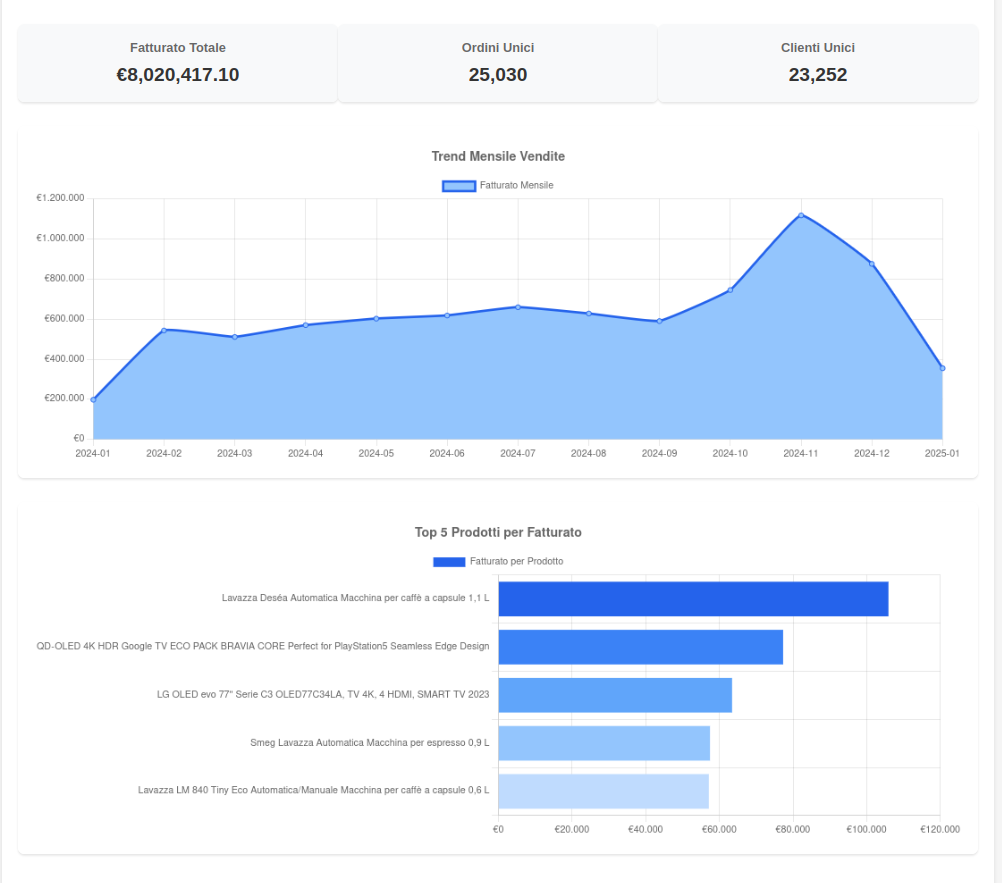
\includegraphics[width=0.9\columnwidth]{Oribea - Esempio di report delle vendite.png}
    \caption{Esempio di report delle vendite fornito da Oribea.}
    \label{fig:oribea-report-example}
\end{figure}

Il report contiene le seguenti statistiche:
\begin{itemize}
    \item \textbf{Fatturato Totale}: il totale delle vendite effettuate nel periodo racchiuso nel dataset;
    \item \textbf{Ordini Unici}: il numero di ordini unici effettuati nel periodo racchiuso nel dataset; questa statistica è necessaria perchè più righe contenenti lo stesso ordine possono essere presenti nel dataset, a causa della possibile presenza di più prodotti nello stesso ordine;
    \item \textbf{Clienti Unici}: il numero di clienti unici che hanno effettuato ordini nel periodo racchiuso nel dataset; questa statistica è necessaria perchè più righe contenenti lo stesso cliente possono essere presenti nel dataset, a causa della possibile presenza di più ordini effettuati dallo stesso cliente.
\end{itemize}

Queste statistiche sono state scelte come base per l'analisi delle vendite, e sono state implementate nel sistema di analisi automatizzato. Successivamente, sono state aggiunte altre statistiche utili, che sono state scelte in base alla loro rilevanza per l'analisi delle vendite e alla loro capacità di fornire informazioni significative. Le statistiche aggiuntive sono le seguenti:
\begin{itemize}
    \item \textbf{Prodotti Unici}: il numero di prodotti unici venduti nel periodo racchiuso nel dataset; questa statistica è necessaria perchè più righe contenenti lo stesso prodotto possono essere presenti nel dataset, a causa della presenza di più ordini effettuati dallo stesso cliente;
    \item \textbf{Spesa Media per Ordine}: la spesa media per ordine, calcolata come il fatturato totale diviso per il numero di ordini unici; questa statistica è utile per comprendere quanto i clienti spendono mediamente per ogni ordine.
\end{itemize}

Successivamente, sono state pensate delle altre elaborazioni statistiche, che però non sono state implementate nel sistema di analisi automatizzato per le ragioni spiegate nelle sezioni \S\ref{sec:recognition-brands} e \S\ref{sec:recognition-categories} legate al \gls{preprocessing}.

A valle di ciò, seppure siano state pensate delle statistiche utili aggiuntive, si è deciso di non implementarle nel sistema di analisi automatizzato. Sono rimaste dunque le cinque statistiche utili descritte in precedenza, che sono state implementate nel sistema di analisi automatizzato e sono state utilizzate per generare il report delle vendite. Queste statistiche sono state scelte in base alla loro rilevanza per l'analisi delle vendite e alla loro capacità di fornire informazioni significative, e sono state ritenute sufficienti per ottenere un'analisi delle vendite efficace e utile.



\section{Valutazione dei grafici utili}

Per poter analizzare le vendite, è fondamentale comprendere quali grafici siano utili per ottenere informazioni significative. Nell'esempio di report delle vendite succitato nell'immagine \ref{fig:oribea-report-example}, sono presenti anche alcuni grafici, che sono stati utilizzati come base per la valutazione dei grafici utili.
I grafici consigliati sono i seguenti:
\begin{itemize}
    \item \textbf{Trend mensile delle vendite}: un grafico a linee che mostra l'andamento delle vendite nel tempo, suddiviso per mese. Questo grafico consente di visualizzare le fluttuazioni delle vendite e di identificare eventuali tendenze stagionali;
    \item \textbf{Top 5 prodotti per fatturato}: un grafico a barre che mostra i cinque prodotti più venduti in termini di fatturato. Questo grafico consente di identificare i prodotti più popolari e redditizi.
\end{itemize}

Il report di esempio ha dunque suggerito l'utilizzo di questi due grafici, che sono stati implementati nel sistema di analisi automatizzato. Non solamente ciò, tale report ha anche suggerito le tipologie di grafici consigliate dall'azienda committente, cioè grafici a linee e a barre, che sono stati quindi scelti per il report per la loro semplicità e chiarezza nella visualizzazione dei dati.

A questo punto, sono stati pensati altri grafici utili, che sono stati implementati nel sistema di analisi automatizzato in parallelo con lo studio del colonne del dataset e del \gls{preprocessing}. I grafici aggiuntivi sono i seguenti:
\begin{itemize}
    \item \textbf{Top 5 clienti per spesa totale}: un grafico a barre che mostra i cinque clienti che hanno speso di più nel periodo racchiuso nel dataset. Questo grafico consente di identificare i clienti più redditizi e di valutare le strategie di fidelizzazione;
    \item \textbf{Trend mensile dei nuovi clienti}: un grafico a linee che mostra l'andamento del numero di nuovi clienti acquisiti nel tempo, suddiviso per mese. Questo grafico consente di valutare l'efficacia delle strategie di marketing e di acquisizione clienti;
    \item \textbf{Trend mennsile della percentuale di nuovi clienti}: un grafico a linee che mostra l'andamento della percentuale di nuovi clienti rispetto al totale dei clienti nel tempo, suddiviso per mese. Questo grafico consente di valutare l'efficacia delle strategie di marketing e di acquisizione clienti in relazione al numero totale di clienti; il valore della percentuale del primo mese è ovviamente 100\%, poiché il numero di nuovi clienti è uguale al numero totale di clienti fino ad allora;
    \item \textbf{Top 5 date per fatturato}: un grafico a barre che mostra le cinque date in cui si è registrato il fatturato più alto. Questo grafico consente di identificare le date più redditizie e di valutare l'efficacia delle strategie di vendita;
    \item \textbf{Top 5 settimane per fatturato}: un grafico a barre che mostra le cinque settimane in cui si è registrato il fatturato più alto. Questo grafico consente di identificare le settimane più redditizie e di valutare l'efficacia delle strategie di vendita.
\end{itemize}

Si nota come sono stati scelti grafici unicamente legati al fatturato, e non a "quantità" o "numero", poiché il fatturato è stata considerata la metrica più importante per l'azienda, cioè quella che fornisce le informazioni più significative. Al contrario, grafici legati a "quantità" o "numero" non sono stati implementati poiché non sono stati ritenuti utili per l'analisi delle vendite.

Molti grafici scelti sono stati legati alla data, poiché si è ritenuto che l'analisi temporale delle vendite fosse fondamentale per comprendere le tendenze e le fluttuazioni delle vendite nel tempo. Da ciò si spiegano le operazioni contemporanee di aggiunta delle colonne legate alla data, descritte sopra nella sezione \S\ref{sec:studio-colonne-dataset}.

Infine, i grafici implementati nel sistema di analisi automatizzato, scelti in base alla loro rilevanza per l'analisi delle vendite e alla loro capacità di fornire informazioni significative, sono stati dunque ritenuti sufficienti per ottenere un'analisi delle vendite efficace e utile.


    \chapter{Sistema di raccomandazione}
\label{cap:sistema-raccomandazione}

\intro{Brevissima introduzione al capitolo}\\

\section{Requisiti per il dataset}

\section{Collaborative filtering}

\section{Similarità}

\section{Rank fusion}

\section{Recbole e Surprise}

\section{Metriche}

\section{Serendipità}

\section{Explainability}

    \chapter{Progettazione e implementazione}
\label{cap:progettazione-implementazione}

\intro{In questo capitolo, vengono descritte le scelte progettuali e le tecniche implementative utilizzate per realizzare il report delle vendite ed il sistema di raccomandazione. Si inizia con una panoramica del flusso delle attività, seguita da una descrizione delle tecnologie e degli strumenti utilizzati. Successivamente, si approfondiscono i vari componenti del sistema sviluppato.}

\section{Flusso delle attività}

\begin{figure}[!h]
    \centering 
    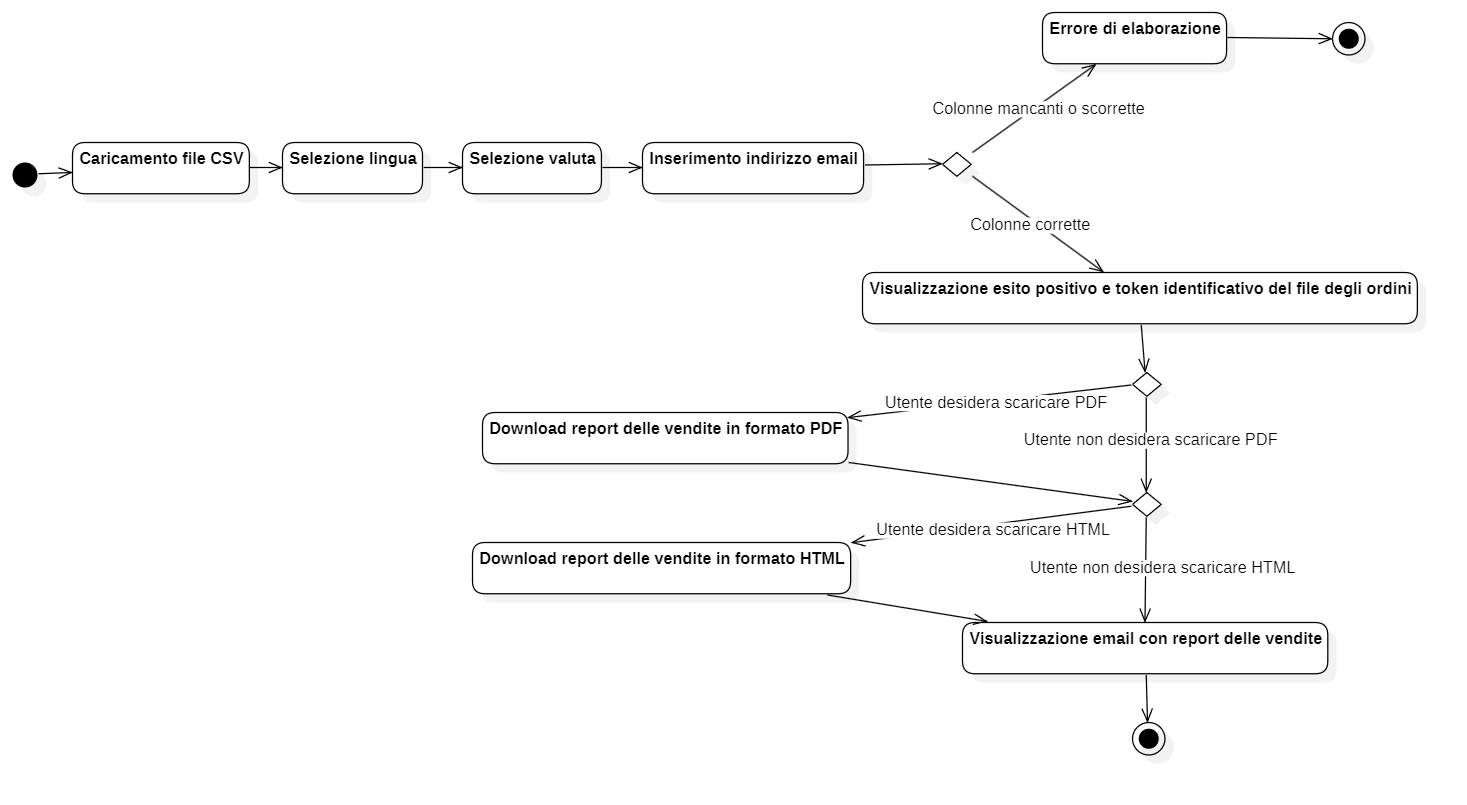
\includegraphics[width=0.9\columnwidth]{activity/Task di analisi delle vendite.png}
    \caption{Flusso delle attività della task di analisi delle vendite}
    \label{fig:activity-sales-analysis}
\end{figure}

Il flusso delle attività per la task di analisi delle vendite è rappresentato nella figura \ref{fig:activity-sales-analysis}. Le attività in sequenza previste dalla task dal lato dell'utente sono:
\begin{itemize}
    \item \textbf{Compilazione dei campi di input}: l'utente deve compilare i campi di input richiesti, cioè deve selezionare il file CSV contenente i dati delle vendite, selezionare la lingua del report e la valuta da utilizzare per i prezzi, e inserire l'indirizzo email a cui inviare il report;
    \item \textbf{Possibili output}: nel caso in cui l'utente abbia inserito correttamente i campi di input e nel caso la task non abbia riscontrato errori, l'utente visualizzerà un messaggio di esito positivo ed un invito a controllare la propria email per il report generato. Viene inoltre segnalata la generazione delle matrici di raccomandazione, e viene visualizzato il token che serve copiare per poter usufruire della task di raccomandazione. In caso la task non vada a buon fine, l'utente visualizzerà un messaggio di errore;
    \item \textbf{I file generati}: la task genera un file PDF ed un file HTML contenenti il report delle vendite, e l'utente ha la possibilità di scaricarli dall'apposita schermata del portale Oribea;
    \item \textbf{La ricezione della mail}: l'utente riceve una mail all'indirizzo email inserito in precedenza, il cui body contiene l'HTML del report, e riporta come allegati il report delle vendite in formato PDF ed HTML; inoltre, viene mostrato anche qui il token che serve copiare per poter usufruire della task di raccomandazione.
\end{itemize}

\begin{figure}[!h]
    \centering 
    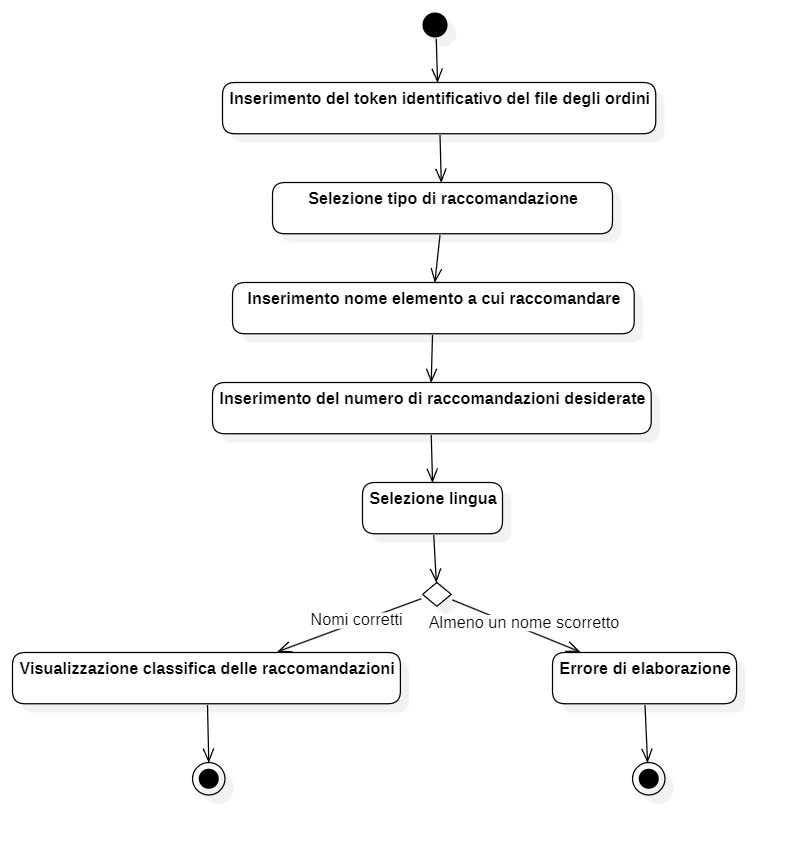
\includegraphics[width=0.9\columnwidth]{activity/Task di raccomandazione di prodotti e clienti.png}
    \caption{Flusso delle attività della task di raccomandazione di prodotti e clienti}
    \label{fig:activity-recommendation-products-customers}
\end{figure}

Il flusso delle attività per la task di raccomandazione di prodotti e clienti è rappresentato nella figura \ref{fig:activity-recommendation-products-customers}. Le attività in sequenza previste dalla task dal lato dell'utente sono:
\begin{itemize}
    \item \textbf{Compilazione dei campi di input}: l'utente deve compilare i campi di input richiesti, cioè deve inserire il token ricevuto nella mail della task di analisi delle vendite, selezionare il tipo di raccomandazione tra "Raccomandare prodotti per un cliente" e "Raccomandare clienti per un prodotto", inserire il nome dell'elemento a cui raccomandare, inserire il numero di raccomandazioni desiderate, e selezionare la lingua con cui presentare la classifica di raccomandazioni;
    \item \textbf{Possibili output}: nel caso in cui l'utente abbia inserito correttamente i campi di input e nel caso la task non abbia riscontrato errori, l'utente visualizzerà la classifica di raccomandazioni generata. In caso la task non vada a buon fine, l'utente visualizzerà un messaggio di errore.
\end{itemize}

Si segnala brevemente, tuttavia, che gli output delle due task non sono stati alla fine l'esatta emulazione di quanto modellato nei diagrammi di attività, ma sono stati modificati in corso d'opera a causa della difficoltà di integrazione con la piattaforma Oribea. In particolare, il download del report delle vendite in formato PDF ed HTML è in realtà stato implementato come download di un file zip (contenente PDF + HTML), poichè la piattaforma Oribea non consente di scaricare più di un file unico come output di una task. Inoltre, il token per accedere alla task di raccomandazione è stato inserito nel file README presente nel file zip, invece che essere mostrato a video come inizialmente previsto. Per quanto riguarda la task di raccomandazione, altrettanto l'output è rappresentato da un file zip, poichè le raccomandazioni sono state generate sia in formato PDF sia in formato JSON, con quest'ultimo che è stato introdotto per favorire una futura estrazione via web dei dati.


\section{Tecnologie e strumenti}
\label{sec:tecnologie-strumenti}

Di seguito viene data una panoramica delle tecnologie e strumenti utilizzati per lo sviluppo delle due task di analisi delle vendite e raccomandazione di prodotti e clienti. Le tecnologie sono state scelte in base alle esigenze del progetto, alla facilità d'uso e alla compatibilità con le altre componenti del sistema.

\subsection{Pandas}
Pandas è una libreria Python per l'analisi dei dati, che fornisce strutture dati e funzioni per la manipolazione e l'analisi dei dati. È stata utilizzata per leggere i file CSV contenenti i dati delle vendite e per elaborare i dati in fase di preprocessing.

\subsection{Babel}
Babel è una libreria Python per la gestione della localizzazione e internazionalizzazione delle applicazioni. È stata utilizzata per gestire le date nel report, in modo da poterle visualizzare nel formato corretto in base alla lingua selezionata dall'utente.

\subsection{Anthropic}
Anthropic è una libreria che consente di interagire con i modelli di linguaggio di grandi dimensioni (\gls{llm}\glsfirstoccur) sviluppati dall'azienda Anthropic tramite le loro API. In particolare, è stato usato il modello Claude 3.7 Sonnet per riconoscere le colonne del file CSV contenente i dati delle vendite, e per generare il resoconto finale che fa da ultimo passaggio del report delle vendite.

\subsection{Matplotlib}
Matplotlib è una libreria Python per la creazione di grafici e visualizzazioni dei dati. È stata utilizzata per generare i grafici presenti nel report delle vendite, in modo da rendere i dati più comprensibili e visivamente accattivanti.

\subsection{Pillow}
Pillow è una libreria Python per la manipolazione delle immagini. È stata utilizzata per generare le immagini dei grafici creati con Matplotlib e per la loro conversione in base64, in modo da poterli inserire nel report delle vendite in formato PDF ed HTML.

\subsection{ReportLab}
ReportLab è una libreria Python per la generazione di documenti PDF, che fornisce una disposizione dinamica del contenuto in pagine. È stata utilizzata per creare il report delle vendite in formato PDF, in modo da renderlo scaricabile dal portale Oribea e da poterlo inviare via email all'utente.

\subsection{Jinja2}
Jinja2 è un motore di template per Python, che consente di generare documenti HTML in modo dinamico. È stata utilizzata per creare il report delle vendite in formato HTML, in modo da renderlo visualizzabile direttamente nel browser e da poterlo anche inviare via email all'utente.

\subsection{Server SMTP interno}
Per l'invio di email, è stato utilizzato un server SMTP messo a disposizione da Oribea, che consente di inviare mail personalizzate senza avere la necessità di utilizzare un indirizzo mail esistente o di collegarsi ad un servizio esterno a pagamento. 

\subsection{Sentence Transformers}
SentenceTransformers è una libreria Python per la creazione di modelli di linguaggio basati su trasformatori, che consente di generare rappresentazioni vettoriali di frasi e documenti. È stata utilizzata per calcolare le similarità tra le descrizioni dei prodotti e i nomi dei prodotti, in modo da poter generare le raccomandazioni. In particolare, è stato utilizzato il modello \emph{all-MiniLM-L6-v2} per generare le rappresentazioni vettoriali delle descrizioni dei prodotti e dei nomi dei prodotti, e per calcolare la similarità tra di essi.

\subsection{Scikit-learn}
Scikit-learn è una libreria Python per il machine learning, che fornisce strumenti per la creazione e l'addestramento di modelli di apprendimento automatico. È stata utilizzata per calcolare la similarità tra le descrizioni dei prodotti e i nomi dei prodotti, in modo da poter generare le raccomandazioni. In particolare, è stato utilizzato il metodo \emph{cosine similarity} per calcolare la similarità tra i vettori delle descrizioni dei prodotti e i vettori dei nomi dei prodotti.

\subsection{Zarr}
Zarr è una libreria Python per la gestione di array multidimensionali, che consente di memorizzare e gestire grandi quantità di dati in modo efficiente. È stata utilizzata per memorizzare su cloud le matrici di raccomandazione generate dalla prima task, in modo da poterle utilizzare successivamente per le raccomandazioni nella seconda task.

\subsection{Google Cloud Storage}
Google Cloud Storage è un servizio di archiviazione di oggetti su cloud fornito da Google. È stato utilizzato per memorizzare i file generati dalla task di analisi delle vendite, come il report in formato PDF ed HTML, e le matrici di raccomandazione generate dalla task di raccomandazione di prodotti e clienti. In particolare, sono stati utilizzati i pacchetti \emph{google.cloud.storage} e \emph{gcsfs} per interagire con il servizio: \emph{google.cloud.storage} è stato utilizzato per scrivere i file, mentre \emph{gcsfs} è stato utilizzato per leggerli.

\subsection{Google Cloud Functions}
Google Cloud Functions è un servizio di calcolo serverless fornito da Google, che consente di eseguire codice in risposta a eventi. È stato utilizzato per caricarvi il codice delle due task di analisi delle vendite e raccomandazione di prodotti e clienti, in modo da poterle eseguire in modo scalabile e senza doversi preoccupare della gestione dei server. Il portale Oribea è configurato per invocare le funzioni di Google Cloud Functions quando l'utente richiede l'esecuzione delle task.

\subsection{Numpy}
Numpy è una libreria Python per il calcolo scientifico, che fornisce strutture dati e funzioni per la manipolazione di array multidimensionali. È stata utilizzata per calcolare le metriche di valutazione delle raccomandazioni.

\subsection{Black}
Black è un formattatore di codice Python che consente di mantenere uno stile di codifica coerente e leggibile. È stato utilizzato per formattare il codice delle due task, in modo da renderlo più leggibile e mantenere uno stile di codifica uniforme.

\subsection{Ruff}
Ruff è un linter per Python che consente di rilevare errori di sintassi e problemi di stile nel codice. È stato utilizzato per verificare la correttezza del codice delle due task, in modo da garantire che fosse privo di errori e conforme agli standard di codifica.

\subsection{MyPy}
MyPy è un tipo di controllo per Python che consente di verificare la correttezza dei tipi di dati nel codice. È stato utilizzato per verificare la correttezza dei tipi di dati delle due task, in modo da garantire che il codice fosse privo di errori di tipo e conforme agli standard di codifica.

\subsection{Pytest}
Pytest è un framework di testing per Python che consente di scrivere e eseguire test automatizzati. È stato utilizzato per testare le due task, in modo da garantire che funzionassero correttamente e fossero prive di errori. I test sono stati scritti in modo da coprire i casi d'uso principali delle due task, e sono stati eseguiti automaticamente durante lo sviluppo per garantire la qualità del codice.


\section{Architettura del sistema}

Prima di cominciare a sviluppare le due task, è stata svolta un'analisi preliminare per definire l'architettura del sistema e le interazioni tra le varie componenti. Siccome le task rappresentano due funzionalità distinte, è stato deciso di svilupparle come due funzioni separate su Google Cloud Functions, e quindi come due diversi progetti il più separati possibile, in modo da poterle gestire indipendentemente e poterle testare separatamente.
Per entrambi i progetti, è stato deciso di utilizzare il linguaggio Python, in modo da poter sfruttare le librerie e gli strumenti già descritti nella sezione \ref{sec:tecnologie-strumenti}.
Inoltre, per entrambi è stato scelto un approccio procedurale a discapito di un approccio orientato agli oggetti, poiché le task sono relativamente semplici e non richiedono una struttura complessa. In aggiunta, è stato deciso di creare dei moduli per organizzare il codice e renderne più facile la lettura e la manutenzione.
I moduli in Python sono rappresentati da cartelle e da file con estensione \emph{.py}, e sono stati utilizzati per raggruppare le funzioni correlate e per separare le responsabilità del codice. In particolare, sono stati creati i moduli descritti di seguito.

Per quanto riguarda la task di analisi delle vendite, sono stati creati i seguenti moduli:
\begin{itemize}
    \item \textbf{preparation}: questo modulo, rappresentato da una cartella, contiene tutti i file necessari per l'inizializzazione del sistema e per l'elaborazione dei dati prima dell'analisi delle vendite. In particolare, contiene i seguenti sottomoduli:
    \begin{itemize}
        \item \textbf{Dependency Injection}: questo modulo, rappresentato da un file \emph{.py}, contiene le funzioni per l'iniezione delle dipendenze necessarie per l'esecuzione della task, come i parametri di configurazione delle \gls{api} verso l'\gls{llm}\glsfirstoccur{} Anthropic e verso il server SMTP interno di Oribea, oltre al modello di embedding per la similarità;
        \item \textbf{Preprocessing}: questo modulo, rappresentato da un file \emph{.py}, contiene le funzioni per il preprocessing dei dati delle vendite; in particolare, contiene la funzione che va a chiamare l'\gls{llm} Anthropic per riconoscere le colonne del file CSV contenente i dati delle vendite, e le funzioni di standardizzazione dei nomi e di sanificazione dei dati;
        \item \textbf{Language Processing}: questo modulo, rappresentato da un file \emph{.py}, contiene le funzioni per l'elaborazione del linguaggio naturale; in particolare, contiene le funzioni per la formattazione delle date e per la selezione dei testi corretti in base alla lingua selezionata dall'utente.
    \end{itemize}
    \item \textbf{report}: questo modulo, rappresentato da una cartella, contiene tutti i file necessari per la generazione del report delle vendite. In particolare, contiene i seguenti sottomoduli:
    \begin{itemize}
        \item \textbf{calculations\_charts}: questo modulo, rappresentato da un file \emph{.py}, contiene le funzioni per il calcolo delle statistiche e dei trend di vendita e per la generazione dei grafici da inserire nel report delle vendite;
        \item \textbf{generate\_report}: questo modulo, rappresentato da un file \emph{.py}, contiene le funzioni per la generazione del report delle vendite in formato PDF ed HTML, utilizzando le librerie ReportLab e Jinja2. Contiene inoltre le funzioni di supporto per la generazione del report, come la funzione di conversione delle immagini dei grafici in base64, la funzione per chiedere all'\gls{llm} Anthropic di generare il resoconto finale del report, e le funzioni per la conversione della risposta ottenuta dall'\gls{llm} da Markdown verso flowables (per il PDF) e verso HTML;
        \item \textbf{send\_email}: questo modulo, rappresentato da un file \emph{.py}, contiene la funzione per l'invio dell'email all'utente allegando il report delle vendite in formato PDF ed HTML, che utilizza il server SMTP interno di Oribea, e una funzione di supporto per la creazione del body della mail.
    \end{itemize}
    \item \textbf{matrices}: questo modulo, rappresentato da un file \emph{.py}, contiene le funzioni per la generazione delle matrici di raccomandazione, che vengono salvate in oggetti di tipo Zarr. In particolare, contiene le funzioni per la generazione delle matrici di raccomandazione basate sugli acquisti e sulla similarità;
    \item \textbf{main}: questo modulo, rappresentato da un file \emph{.py}, contiene la funzione principale \emph{main} che viene eseguita quando la task viene invocata, e che coordina l'esecuzione delle altre funzioni dei moduli scritti in precedenza. Inoltre, tramite delle funzioni apposite, effettua l'upload in Google Cloud Storage dei file generati dalla task, come il report delle vendite in formato PDF ed HTML e le matrici di raccomandazione. Infine, il \emph{main} restituisce l'output della task, cioè una cartella compressa contenente il report delle vendite in formato PDF ed HTML, ed un file README che contiene il token per accedere alla task di raccomandazione di prodotti e clienti.
\end{itemize}

Per quanto riguarda la task di raccomandazione di prodotti e clienti, sono stati creati i seguenti moduli:
\begin{itemize}
    \item \textbf{prediction}: questo modulo, rappresentato da una cartella, contiene tutti i file necessari per la predizione delle raccomandazioni. In particolare, contiene i seguenti sottomoduli:
    \begin{itemize}
        \item \textbf{predictor}: questo modulo, rappresentato da un file \emph{.py}, contiene le funzioni dirette per la predizione delle raccomandazioni, che utilizzano le matrici di raccomandazione generate dalla task di analisi delle vendite. Esso contiene anche l'algoritmo di rank fusion, che combina assieme le raccomandazioni ottenute dalle matrici;
        \item \textbf{filter}: questo modulo, rappresentato da un file \emph{.py}, contiene le funzioni per il filtraggio delle raccomandazioni, in modo da rimuovere, a seconda del caso, i prodotti già acquistati dall'utente ricevuto in input oppure gli utenti che hanno già acquistato il prodotto ricevuto in input;
        \item \textbf{make\_prediction}: questo modulo, rappresentato da un file \emph{.py}, contiene le funzioni per la creazione della predizione delle raccomandazioni, che utilizzano le funzioni dei moduli \emph{predictor} e \emph{filter} per generare la classifica di raccomandazioni. Contiene inoltre una funzione di explanation che stampa su console i passaggi intermedi della predizione, per facilitare il debug e la comprensione del funzionamento della task;
        \item \textbf{build\_output}: questo modulo, rappresentato da un file \emph{.py}, costruisce l'output della task, cioè chiama una funzione che genera un file JSON con le raccomandazioni e i punteggi, e una funzione che genera un PDF dove viene riportato il ranking predetto.
    \end{itemize}
    \item \textbf{evaluation}: questo modulo, rappresentato da una cartella, contiene tutti i file necessari per la valutazione delle raccomandazioni. In particolare, contiene i seguenti sottomoduli:
    \begin{itemize}
        \item \textbf{metrics}: questo modulo, rappresentato da un file \emph{.py}, contiene le funzioni per il calcolo delle metriche di valutazione delle raccomandazioni. Queste metriche vengono calcolate confrontando le raccomandazioni generate dalla task con le vendite passate dei prodotti o dei clienti;
        \item \textbf{check\_metrics}: questo modulo, rappresentato da un file \emph{.py}, contiene le funzioni per il controllo delle metriche di valutazione delle raccomandazioni, in modo da verificare se le raccomandazioni generate sono valide e soddisfacenti. In particolare, vengono richiamate le funzioni del modulo \emph{metrics} per calcolare le metriche di valutazione, che vengono stampate su console, assieme al loro significato, per facilitare il debug e la comprensione del funzionamento del sistema di raccomandazione.
    \end{itemize}
    \item \textbf{main}: questo modulo, rappresentato da un file \emph{.py}, contiene la funzione principale \emph{main} che viene eseguita quando la task viene invocata, e che coordina l'esecuzione delle altre funzioni dei moduli scritti in precedenza. Inizialmente, essa si occupa di cercare in Google Cloud Storage il bucket identificato dal token ricevuto in input, e di caricare le matrici di raccomandazione da esso. Successivamente, il \emph{main} richiama le funzioni del modulo \emph{prediction/make\_prediction} per generare la classifica di raccomandazioni, e quelle del modulo \emph{evaluation/check\_metrics} per calcolare le metriche di valutazione di tali raccomandazioni. Infine, il \emph{main} restituisce l'output della task, cioè una cartella compressa contenente le raccomandazioni in formato JSON e PDF.
\end{itemize}

Sono stati appena descritti i moduli contenuti dentro la cartella \emph{src} delle task, che rappresentano il cuore del codice dei due progetti. Attorno ad esse, per ciascuna task, è stata creata una struttura di cartelle e file che rappresentano la configurazione del progetto, le dipendenze necessarie per l'esecuzione delle task, i test automatizzati e un file main per collegarsi al servizio Cloud Functions. In particolare, sono stati creati i seguenti file:
\begin{itemize}
    \item \textbf{requirements.txt}: questo file contiene le dipendenze necessarie per l'esecuzione delle task, che vengono installate automaticamente quando si carica il codice su Google Cloud Functions;
    \item \textbf{.gcloudignore}: questo file contiene le regole per ignorare i file e le cartelle che non devono essere caricati su Google Cloud Functions, come i file di test e i file di configurazione locali;
    \item \textbf{tests}: questa cartella contiene i test automatizzati per le due task, che vengono eseguiti automaticamente durante lo sviluppo per garantire la qualità del codice. I test sono scritti utilizzando il framework Pytest, e sono organizzati in moduli separati per ciascuna task;
    \item \textbf{main.py}: questo file contiene il codice principale per collegarsi al servizio Cloud Functions, e richiama la funzione principale della task corrispondente;
    \item \textbf{logger.py}: questo file contiene la configurazione dell'oggetto logger delle due task, che viene utilizzato per tracciarne l'esecuzione e per facilitarne il debug in caso di errori. I log vengono scritti su console e possono essere visualizzati tramite il servizio di logging di Google Cloud;
    \item \textbf{.env}: questo file contiene le variabili d'ambiente necessarie per l'esecuzione delle task;
    \item \textbf{pyproject.toml}: questo file contiene la configurazione del progetto, come il nome del progetto, la versione, la descrizione e le dipendenze necessarie per l'esecuzione delle task. Inoltre, contiene le configurazioni per i tool di formattazione e linting del codice, come Black, Ruff e MyPy;
    \item \textbf{pytest.ini}: questo file contiene la configurazione per Pytest, il framework di testing utilizzato per i test automatizzati delle due task. In particolare, contiene la configurazione della coverage a 75\% per i test, e la configurazione per eseguire i test per l'\gls{llm} separatamente rispetto ai test "classici";
    \item \textbf{file run\_*.bat}: script per l'esecuzione dell'analisi statica del codice, che eseguono i tool di formattazione e linting Black, Ruff e MyPy. Questi script sono stati creati per facilitare l'esecuzione di questi ultimi tool, in modo da poterli consultare facilmente durante lo sviluppo;
    \item \textbf{deploy.bat}: questo file contiene lo script per l'esecuzione del complesso comando di deployment su Google Cloud Functions.
\end{itemize}

Successivamente, verso il termine dello stage, a queste cartelle contenenti i progetti backend delle due task si sono aggiunte le due cartelle dei corrispettivi progetti frontend, la cui realizzazione era desiderabile (non obbligatoria), che sono stati sviluppati per permettere all'utente di interagire con le task tramite un'interfaccia diversa da quella standard della piattaforma Oribea, e per introdurre la validazione dell'input. La struttura di queste cartelle corrisponde alla struttura standard di un progetto React, i cui componenti sono approfonditi nella sezione \S\ref{sec:frontend}.



\section{Preprocessing}
\label{sec:preprocessing}

Il preprocessing dei dati delle vendite è un passaggio fondamentale per garantire che i dati siano pronti per l'analisi e la generazione del report, e anche perchè sia possibile crearci le matrici di raccomandazione.
In questa sezione, vengono descritti i passaggi principali del preprocessing, che sono stati implementati nella task di analisi delle vendite.

Una volta ricevuto in input il file csv con i dati delle vendite, il suo contenuto viene prelevato mediante Pandas e salvato in oggetto Dataframe. La prima cosa che è stato scelto di fare è una pulizia e sanificazione dei dati, in modo da rimuovere eventuali errori o anomalie. In particolare, vengono rimosse eventuali righe duplicate e vengono tolti gli spazi bianchi all'inizio e alla fine nei valori di tipo stringa.

A questo punto, procedere meccanicamente non è più possibile, poichè ogni file csv di vendite possiede i propri specifici nomi delle colonne, che possono essere scritti in modi diversi, e che non sono standardizzati. Per questo motivo, è stato scelto di utilizzare un modello di \gls{llm} per riconoscere le colonne del file CSV, in modo da poterle standardizzare e rendere più facili da gestire. In particolare, viene utilizzato il modello Claude 3.7 Sonnet di Anthropic per riconoscere le colonne del file CSV e restituirne i nomi corrispondenti alle categorie prestabilite, in modo da poterci svolgere la successiva analisi delle vendite e generazione delle matrici di raccomandazione. Il modello viene chiamato tramite l'\gls{api} di Anthropic, e vengono passati i nomi delle colonne e un'anteprima del loro contenuto come input. Il modello viene istruito con un apposito header a restituire i nomi delle colonne che facciano da parametri ad alcune particolari funzioni, cioè:
\begin{itemize}
    \item \textbf{prepare\_fundamental\_columns}: questa funzione prende in input i nomi delle colonne fondamentali del file CSV, cioè gli id di clienti e prodotti, le date degli ordini, i prezzi e le quantità, modifica tali colonne nel dataframe standardizzandone i nomi, e restituisce il dataframe modificato. Vengono inoltre formattate numericamente le colonne dei prezzi e delle quantità (anche tramite la funzione di supporto \texttt{replace\_and\_to\_numeric}), in modo da poterle utilizzare per i calcoli successivi, e vengono rimosse le righe con almeno un valore vuoto;
    \item \textbf{prepare\_denominative\_columns}: questa funzione prende in input i nomi delle colonne denominative del file CSV, cioè le colonne contenenti le descrizioni dei prodotti e dei clienti, e modifica tali colonne nel dataframe standardizzandone i nomi. È possibile che l'\gls{llm} associ più colonne allo scopo descrittivo di un prodotto o di un cliente, e in tal caso queste colonne vengono concatenate in una sola, che contiene così la descrizione completa. Inoltre, vengono rimosse le righe con almeno un valore vuoto, e tutte le colonne, fondamentali e denominative, vengono ordinate tra loro in modo da avere un ordine standardizzato;
    \item \textbf{extract\_date\_components}: questa funzione prende in input il nome della colonna contenente il timestamp degli ordini e un parametro che indica se nel timestamp viene prima il valore del giorno o del mese, e crea quattro nuove colonne nel dataframe, che contengono rispettivamente il giorno, la settimana, il mese e l'anno dell'ordine. Inoltre, viene gestita la possibilità che la stessa colonna di timestamp presenti i suoi valori in due formati diversi, provando un secondo tentativo di parsing della data in caso di errore nel primo tentativo. Se neanche il secondo tentativo va a buon fine, vengono rimosse le righe contenenti i timestamp non validi.
\end{itemize}

Terminata la parte di preprocessing dipendente dal dataset, vengono effettuate alcune ultime elaborazioni meccaniche:
\begin{itemize}
    \item \textbf{create\_iso\_date\_columns}: questa funzione crea due nuove colonne nel dataframe, che contengono rispettivamente la data in formato ISO e il mese in formato ISO, a partire dalle colonne del giorno, del mese e dell'anno create in precedenza;
    \item \textbf{sort\_values}: questa funzione ordina il dataframe in base alla colonna della data ISO degli ordini, in modo da avere le righe ordinate cronologicamente;
    \item \textbf{maintain\_first\_name}: questa funzione prende in input una coppia di colonne contenenti id e nomi di una stessa entità, e fa un modo che ad uno stesso id sia sempre associato un solo nome, prendendo il primo nome trovato per quell'id e mantenendolo per tutte le righe in cui quell'id compare. In questo modo, si evita di avere nomi diversi associati allo stesso id, come era capitato per alcuni prodotti, che potrebbero causare errori durante l'analisi dei dati;
    \item \textbf{delete\_columns\_except}: questa funzione prende in input una lista di nomi di colonne da mantenere nel dataframe, e rimuove tutte le altre colonne. In questo modo, si evita di avere colonne inutili o ridondanti nel dataframe, che potrebbero causare confusione durante l'analisi dei dati.
\end{itemize}

Dopo aver eseguito tutte queste operazioni, il dataframe è pronto per essere utilizzato per l'analisi delle vendite e la generazione delle matrici di raccomandazione. In particolare, il dataframe contiene le colonne fondamentali e denominative standardizzate, le colonne con i componenti della data degli ordini, e le colonne con i prezzi e le quantità formattate numericamente. Inoltre, il dataframe è ordinato cronologicamente in base alla data degli ordini, e contiene solo le colonne necessarie per l'analisi dei dati.

Inizialmente, per migliorare il report delle vendite con ulteriori informazioni sui prodotti, era stato pensato di aggiungere due altre colonne al dataframe, una per la marca e una per la categoria del prodotto. Tuttavia, come descritto nelle sezioni \S\ref{sec:recognition-brands} e \S\ref{sec:recognition-categories}, ciò non è stato possibile.


\subsection{Riconoscimento delle marche}
\label{sec:recognition-brands}

Per poter analizzare le vendite in modo più dettagliato, è stato pensato di introdurre una colonna "Marca" nei dataset, che potesse contenere il nome della marca del prodotto presente in tale riga. Per ottenere ciò, era dunque necessario sviluppare un sistema di riconoscimento delle marche. Sono state provate le seguenti strategie:
\begin{itemize}
    \item \textbf{Riconoscimento tramite dizionario}: è stato creato un dizionario contenente le marche più comuni, ma si è rivelato poco efficace, poiché molte marche non erano presenti nel dizionario e il riconoscimento era limitato;
    \item \textbf{Riconoscimento tramite regex}: è stato provato a utilizzare delle espressioni regolari per riconoscere le marche, ma si è rivelato poco efficace, poiché molte marche non seguivano uno schema comune e il riconoscimento era limitato;
    \item \textbf{Riconoscimento tramite modelli di \gls{ml}\glsfirstoccur{}}: è stato pensato di creare un modello di \gls{ml} per riconoscere le marche, ma si è rivelato poco efficace, poiché il dataset non era sufficientemente grande e vario per addestrare un modello affidabile, e soprattuto non erano disponibili le etichette necessarie per un addestramento supervisionato;
    \item \textbf{Riconoscimento tramite modelli di \gls{ner}\glsfirstoccur{}}: è stato provato ad utilizzare un modello di \gls{ner} sulle descrizioni dei prodotti e a selezionare le entità segnalate di tipo \emph{ORG} (organizzazione), ma si è rivelato poco efficace, poiché il modello non era stato addestrato specificamente per questo compito e il riconoscimento era limitato;
    \item \textbf{Riconoscimento tramite \gls{llm}\glsfirstoccur{}}: è stato provato ad utilizzare un modello di linguaggio di grandi dimensioni (\gls{llm}) per riconoscere le marche, e si è rivelato mediamente efficace, ma il riconoscimento di ciascuna marca richiedeva troppo tempo e tantissime chiamate \gls{api}\glsfirstoccur{}; allora, è stato fatto un tentativo di raggruppamento di più descrizioni da inviare assieme per il riconoscimento di più marche contemporaneamente, ma si è rivelato poco efficace, poiché il modello ogni tanto si dimenticava di alcune marche o ne aggiungeva qualcuna in più, totalmente senza motivo (avvenivano cioè le cosidette "allucinazioni").
\end{itemize}

Dunque, si è deciso di non implementare il riconoscimento delle marche nel sistema di analisi automatizzato, poiché non era possibile garantire un riconoscimento affidabile e preciso.


\subsection{Riconoscimento delle categorie}
\label{sec:recognition-categories}

Per poter analizzare le vendite in modo più dettagliato, è stato pensato di introdurre una colonna "Categoria" nei dataset, che potesse contenere il nome della categoria del prodotto presente in tale riga. Per ottenere ciò, era dunque necessario sviluppare un sistema di riconoscimento delle categorie.

Escluse le opzioni già descritte nella sezione \S\ref{sec:recognition-brands} per il riconoscimento delle marche, è stato pensato di utilizzare un modello \gls{kmeans}\glsfirstoccur{} per raggruppare i prodotti in base alle loro descrizioni, in modo da ottenere delle categorie. Tuttavia, ciò si è rivelato poco efficace, poiché il modello non era in grado di raggruppare i prodotti in categorie in modo affidabile e preciso, e il numero di categorie era troppo elevato per poterle gestire manualmente.

Dunque, si è deciso di non implementare il riconoscimento delle categorie nel sistema di analisi automatizzato, poiché non era possibile garantire un riconoscimento affidabile e preciso.


È stata svolta anche un'altra operazione di preprocessing, che però non è stata implementata nel modulo dedicato.
Infatti, durante lo sviluppo dei grafici per il report delle vendite, è stato necessario gestire il caso in cui prodotti diversi abbiano lo stesso nome: è stato deciso di inserire un suffisso numerico (es.: (1), (2), ...) ai nomi di prodotto identici, in modo da poterli distinguere. Questa modifica si è però rivelata molto lenta ed inefficiente da svolgere su tutto il dataframe, e quindi è stato deciso di svolgerla solo sui nomi dei prodotti che venivano utilizzati per i grafici.
Questa operazione è stata dunque svolta direttamente nel modulo \emph{report/calculations\_charts}, dove vengono generati i grafici, e non nel modulo \emph{preparation/preprocessing}, dove viene svolto il preprocessing dei dati delle vendite.



\section{Language processing}
\label{sec:language-processing}

In ogni applicazione che gestisce testi in lingue diverse è fondamentale avere un sistema di elaborazione del linguaggio naturale che consenta di gestire correttamente le lingue e le loro specificità. Nel caso della task di analisi delle vendite, è stato necessario implementare un sistema di language processing che consentisse di gestire correttamente le date e i testi in base alla lingua selezionata dall'utente.

Le lingue italiano, inglese, francese, spagnolo e tedesco sono le uniche permesse nel sistema: ne viene selezionata una dall'utente tramite un menù a tendina presente nell'interfaccia grafica della piattaforma Oribea. Esse sono state scelte in quanto sono le lingue più parlate al mondo e le più comuni tra gli utenti del piattaforma.

Per quanto riguarda le date, è stato necessario implementare un sistema di formattazione che consentisse di gestirle correttamente in base alla lingua selezionata dall'utente. In particolare, oltre ad avere le date in formato ISO (le cui relative colonne sono state ottenute nell'elaborazione descritta in \S\ref{sec:preprocessing}), in modo da poterle utilizzare per i calcoli, occorreva anche un sistema che consentisse di gestire le date in formato localizzato, in modo da poterle visualizzare correttamente nel report delle vendite.
Le relative colonne sono state ottenuto utilizzando la libreria \emph{babel} di Python, che consente di gestire le lingue e le loro specificità. In particolare, è stato utilizzato il modulo \emph{babel.dates} e la funzione \emph{format\_dates} per formattare le date in base alla lingua selezionata dall'utente.

Per quanto riguarda i testi presenti nel report delle vendite, è stato necessario implementare un sistema di selezione dei testi in base alla lingua selezionata dall'utente. Considerata la relativa semplicità del report, è stato deciso di non utilizzare dei file di lingua, bensì sono stati semplicemente scritti i testi selezionabili in modo hardcoded direttamente nel codice.
La funzione dedicata ha dunque il compito di restituire un dizionario che presenta i testi nella lingua corretta accessibili tramite le chiavi corrispondenti. Ad esempio, per inserire il titolo del report, si deve accedere alla chiave \emph{title} del dizionario \texttt{report\_language\_dependent\_data}, che permette di ottenere il titolo nella lingua selezionata dall'utente.

Un'altra operazione di language processing riguarda la selezione del testo che la task deve riportare in output per descrivere le operazioni svolte, presentare i risultati ottenuti e invitare l'utente a usufruire delle matrici di raccomandazione mediante la task apposita. Per quest'ultimo proposito, in questo testo viene anche riportato il token che l'utente deve utilizzare per accedere alle matrici, che sono state salvate su Google Cloud Storage.
L'ultima operazione di language processing riguarda la selezione dell'oggetto e del body per la mail che viene inviata all'utente allegando il report delle vendite in formato PDF ed HTML.
Anche in questi ultimi due casi, per semplicità è stato deciso di non utilizzare dei file di lingua, bensì sono stati semplicemente hardcodati i testi direttamente nel codice.


\section{Report}

Il report delle vendite è il risultato finale della task di analisi delle vendite, e viene generato in formato PDF ed HTML. Il report contiene le statistiche ed i grafici che rappresentano i trend delle vendite nel tempo, e un resoconto finale generato dall'\gls{llm} Anthropic.
In questa sezione, vengono descritti i passaggi principali che hanno portato alla generazione del report.

\subsection{PDF}

Il report in formato PDF, in quanto requisito obbligatorio del progetto, è stato sviluppato per primo. Per la sua generazione, sono state prese in considerazione le seguenti librerie:
\begin{itemize}
    \item \textbf{ReportLab}: è una libreria Python per la generazione di documenti PDF, che consente di creare documenti complessi e personalizzati. È stata presa in considerazione per la sua capacità di creare report strutturati con layout avanzati, supporto per grafici e immagini, e controllo dettagliato della formattazione;
    \item \textbf{FPDF}: è una libreria Python per la generazione di documenti PDF, che consente di creare documenti semplici e veloci. È stata presa in considerazione per la sua semplicità di utilizzo e leggerezza, adatta per la generazione rapida di documenti con layout basilari;
    \item \textbf{PyPDF2}: è una libreria Python per la manipolazione di documenti PDF, che consente di unire, dividere e modificare documenti PDF esistenti. È stata presa in considerazione per la possibilità di combinare più sezioni del report o integrare template PDF preesistenti;
    \item \textbf{PDFRW}: è una libreria Python per la manipolazione di documenti PDF, che consente di leggere e scrivere documenti PDF esistenti. È stata presa in considerazione come alternativa a PyPDF2 per operazioni di manipolazione e modifica di documenti PDF già formattati.
\end{itemize}

Alla fine, è stata scelta la libreria ReportLab per la generazione del report in formato PDF, poiché consente di gestire le pagine in modo dinamico e semplice: infatti, all'inserimento di un nuovo flowable (un elemento grafico), ReportLab si occupa automaticamente di creare una nuova pagina se necessario, e di gestire il layout del documento in modo automatico, a differenza di altre librerie che richiedono una gestione manuale delle pagine. Inoltre, ReportLab consente di inserire immagini e grafici in modo semplice e veloce, e di gestire la formattazione del testo in modo avanzato.

Per gestire l'inserimento nel report del resoconto generato dall'\gls{llm}, è stato necessario creare una funzione che consentisse di convertire il testo in formato Markdown in flowables di ReportLab. Questa conversione è stata realizzata manualmente, poichè gli output dell'\gls{llm} come resoconto sono molto semplici e non contengono elementi complessi come tabelle o liste, e quindi non era necessario utilizzare una libreria esterna per la conversione.


\subsection{HTML}

Dopo aver sviluppato il report in formato PDF ed aver risolto un buon numero di requisiti obbligatori, è stato deciso di sviluppare anche il report in formato HTML, in modo da poterlo visualizzare direttamente nel browser ed avere la possibilità, in futuro, di integrarlo in una pagina web. Per la sua generazione, sono state prese in considerazione le seguenti librerie:
\begin{itemize}
    \item \textbf{Jinja2}: è un motore di template per Python, che consente di generare documenti HTML in modo dinamico e personalizzato. È stata presa in considerazione per la sua capacità di creare template HTML strutturati e riutilizzabili, con supporto per variabili, cicli e condizioni;
    \item \textbf{Mako}: è un altro motore di template per Python, simile a Jinja2, che consente di generare documenti HTML in modo dinamico e personalizzato. È stata presa in considerazione per la sua sintassi semplice e leggibile, e per le sue funzionalità avanzate di templating;
    \item \textbf{Dominate}: è una libreria Python per la generazione di documenti HTML, che consente di creare documenti HTML in modo semplice e veloce, utilizzando una sintassi basata su Python. È stata presa in considerazione per la sua facilità d'uso e per la sua capacità di generare documenti HTML ben formattati;
    \item \textbf{Yattag}: è una libreria Python che permette di generare documenti XML/HTML attraverso un approccio programmatico con metodi Python dedicati. È stata presa in considerazione per la sua sintassi intuitiva che evita la necessità di scrivere tag HTML manualmente e per il suo controllo preciso sulla struttura del documento.
\end{itemize}

Prima di tutto è stato necessario scegliere l'approccio con cui creare l'HTML, tra motore di template e generazione programmatica. È stato allora scelto di utilizzare un motore di template, poiché consente di separare la logica di generazione del report dalla struttura del documento, rendendo il codice più leggibile e manutenibile. Tra i motori di template considerati, è stato scelto Jinja2, poiché è il più diffuso e supportato, e consente di creare template HTML strutturati e riutilizzabili.

Per la generazione del report in formato HTML, è stato dunque creato un template Jinja2 contenente la struttura del documento e i segnaposto per le variabili. Il template è stato progettato per essere facilmente personalizzabile, in modo da poter modificare la struttura del report senza dover riscrivere il codice di generazione. Inoltre, il template consente di inserire le immagini dei grafici codificate in base64, in modo da poterle visualizzare direttamente nel report senza doverle salvare separatamente.

Anche in questo caso, per inserire il resoconto generato dall'\gls{llm}, è stato necessario creare una funzione che consentisse di convertire il testo in formato Markdown in HTML. Questa conversione è stata altrettanto realizzata manualmente, per il suddetto motivo legato alla semplicità del resoconto.


\section{Invio di email}

Il più opzionale dei requisiti del progetto riguardanti l'output della task di analisi delle vendite è l'invio di una mail all'utente con il report allegato. Dunque, al termine dello sviluppo della task, è stato implementato anche questo requisito, che consente non solo un'altra modalità di recupero del report, ma anche un'altra modalità di recupero del token per accedere alle matrici di raccomandazione, il quale viene riportato nel corpo della mail.

Di fronte a questo requisito, sono state prese in considerazione varie possibilità.
Inizialmente, si era pensato di inviare la mail da un indirizzo di posta elettronica esistente, ma, dopo consultazione con il tutor, per evitare la condivisione di credenziali riservate, si è deciso invece di contattare tramite \gls{api} un server SMTP esterno che permetta di inviare mail inserendo un indirizzo di posta elettronica di mittente a piacere. Questo servizio non ha bisogno di un account di posta elettronica esistente, dunque come mittente è stato scelto l'indirizzo \texttt{no-reply@oribea.ai}, il cui nome invita l'utente a non rispondere, considerato che la risposta non verrebbe ricevuta.

La questione successiva è stata la scelta del server SMTP da utilizzare, di fondamentale importanza in quanto rappresenta un investimento economico per l'azienda.
Tuttavia, dopo una ulteriore consultazione con il tutor, si è deciso di utilizzare un server SMTP interno, sviluppato direttamente dall'azienda Oribea appositamente per il progetto, che consenta di inviare mail senza dover pagare un abbonamento.

Una volta realizzato il server SMTP e testato tramite cURL, è stato possibile implementare una funzione di contatto che imitasse appunto la stringa di comando cURL, e che inviasse una mail all'utente con i file di report allegati. Questa funzione è stata realizzata utilizzando la libreria requests, ed è stata inserita nel modulo \emph{report/send\_mail}.

Un problema che si è presentato durante il testing del contatto via codice è stata la codifica dei caratteri speciali (come ad esempio le lettere accentate) nell'oggetto e nel corpo delle mail, che non veniva gestita correttamente dal server SMTP interno. Per risolvere è stato tuttavia sufficiente segnalare il problema al tutor, che ha risolto modificando appositamente il server, garantendo così il supporto all'invio di mail in lingue diverse dall'inglese e contenenti caratteri speciali.

Attualmente il server SMTP interno di Oribea è hostato su una macchina dev, e quindi servizi come Gmail e Outlook considerano le mail inviate come spam, e non le recapitano all'utente. Tuttavia, il server SMTP è stato testato con successo e funziona correttamente verso gli altri provider, come ad esempio Libero, e quindi si prevede che in futuro verrà hostato su una macchina di produzione in modo da poter inviare le mail senza problemi di spam.


\section{Le matrici di raccomandazione}

1. Crosstab di Pandas
2. Cosine similarity di Scikit-learn
3. Pandas Vectorized Ops per la norma

\subsection{Formato di archiviazione delle matrici}

Considerati l'elevato consumo di spazio e la lentezza di accesso ai dati delle matrici di raccomandazione salvate come file CSV, si è deciso di svolgere un'analisi preliminare per valutare il formato di archiviazione più adatto. Sono stati presi in considerazione i seguenti formati:
\begin{itemize}
    \item \textbf{CSV}: il formato CSV (Comma-Separated Values) è un formato di testo semplice e ampiamente utilizzato per la memorizzazione di dati tabellari. È stato preso in considerazione per la sua semplicità, portabilità e compatibilità con numerosi strumenti di analisi dati;
    \item \textbf{HDF5}: HDF5 (Hierarchical Data Format version 5) è un formato binario progettato per la gestione efficiente di grandi quantità di dati complessi e strutturati. È stato valutato per le sue capacità di compressione, accesso rapido e supporto a dataset multidimensionali;
    \item \textbf{NPY}: il formato NPY è il formato binario nativo di NumPy per la memorizzazione di array multidimensionali. È stato considerato per la sua efficienza nello storage e nella lettura di array numerici in ambiente Python;
    \item \textbf{Parquet}: Parquet è un formato di archiviazione colonnare ottimizzato per l'analisi di grandi volumi di dati. È stato preso in considerazione per le sue prestazioni elevate, la compressione e la compatibilità con diversi framework di big data;
    \item \textbf{Zarr}: Zarr è un formato per la memorizzazione di array multidimensionali che supporta la compressione e l'accesso parallelo ai dati. È stato valutato per la sua scalabilità, flessibilità e facilità di integrazione con sistemi cloud.
\end{itemize}

Sono stati dunque sviluppati dei test automatizzati per confrontare le prestazioni di lettura dei vari formati e lo spazio occupato su disco. I tempi di scrittura non sono stati considerati, poiché le matrici di raccomandazione vengono generate una sola volta e poi salvate su Google Cloud Storage, dove rimangono per essere utilizzate in seguito. I dataset che sono stati utilizzati per i test sono stati scelti cercando di variare la dimensione e la densità delle matrici, e sono qui di seguito elencati in ordine crescente di dimensione della matrice:
\begin{table}[h]
    \centering
    \begin{tabular}{|l|c|}
        \hline
        \textbf{Dataset} & \textbf{Dimensioni della matrice} \\
        \hline
        Feroze & 10 $\times$ 10 \\
        Vaghasiya & 2.172 $\times$ 268 \\
        Anwer & 795 $\times$ 10.292 \\
        Delikkaya & 35.389 $\times$ 1.000 \\
        Orders\_export & 23.389 $\times$ 4.114 \\
        Cornelius & 14.095 $\times$ 15.000 \\
        \hline
    \end{tabular}
    \caption{Dataset utilizzati per il confronto dei formati di archiviazione delle matrici di raccomandazione}
    \label{tab:dataset-matrici}
\end{table}

I risultati dei test di memoria occupata su disco sono stati i seguenti:

\begin{figure}[!h]
    \centering
    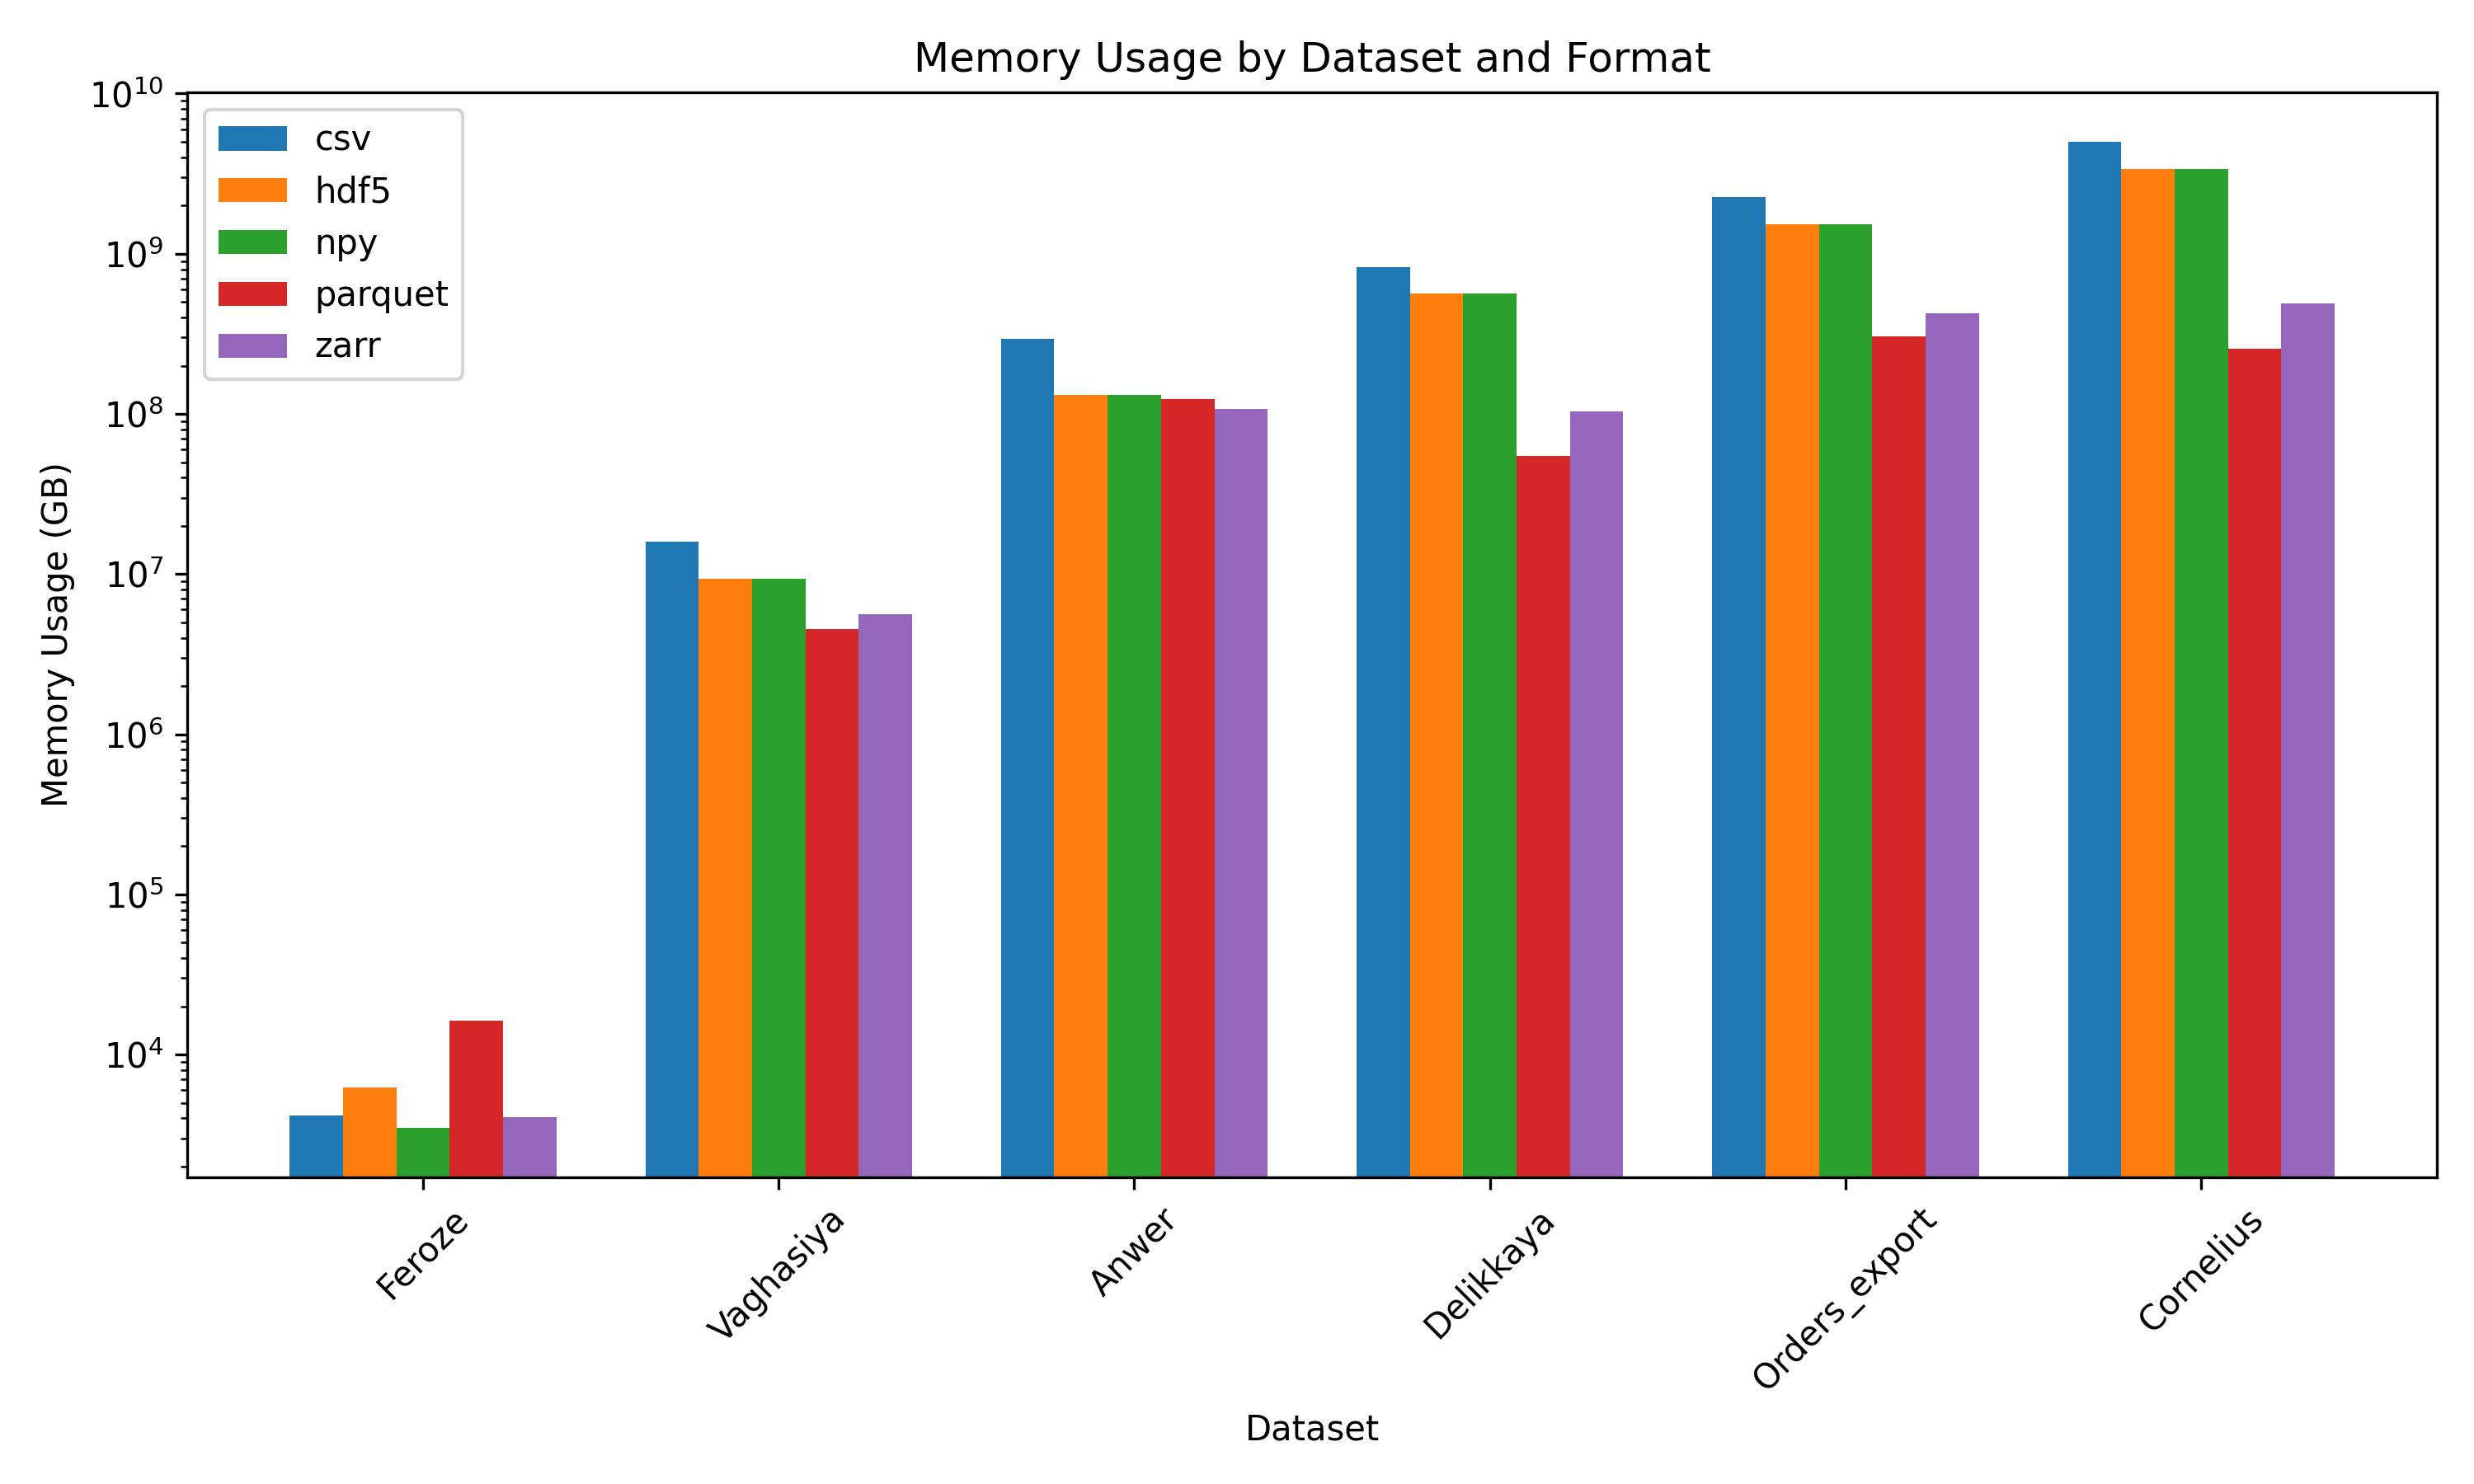
\includegraphics[width=0.9\columnwidth]{benchmark/memory_usage_by_dataset_and_format.png}
    \caption{Utilizzo della memoria dei formati di archiviazione delle matrici di raccomandazione}
    \label{fig:memory-usage-recommendation-matrices}
\end{figure}

Si evince dunque che i dataset sono classificabili all'incirca così in ordine crescente di spazio occupato su disco:
\begin{enumerate}
    \item Parquet;
    \item Zarr;
    \item NPY;
    \item HDF5;
    \item CSV.
\end{enumerate}

I risultati dei test di velocità di lettura dei vari formati sono stati i seguenti:
\begin{figure}[!h]
    \centering
    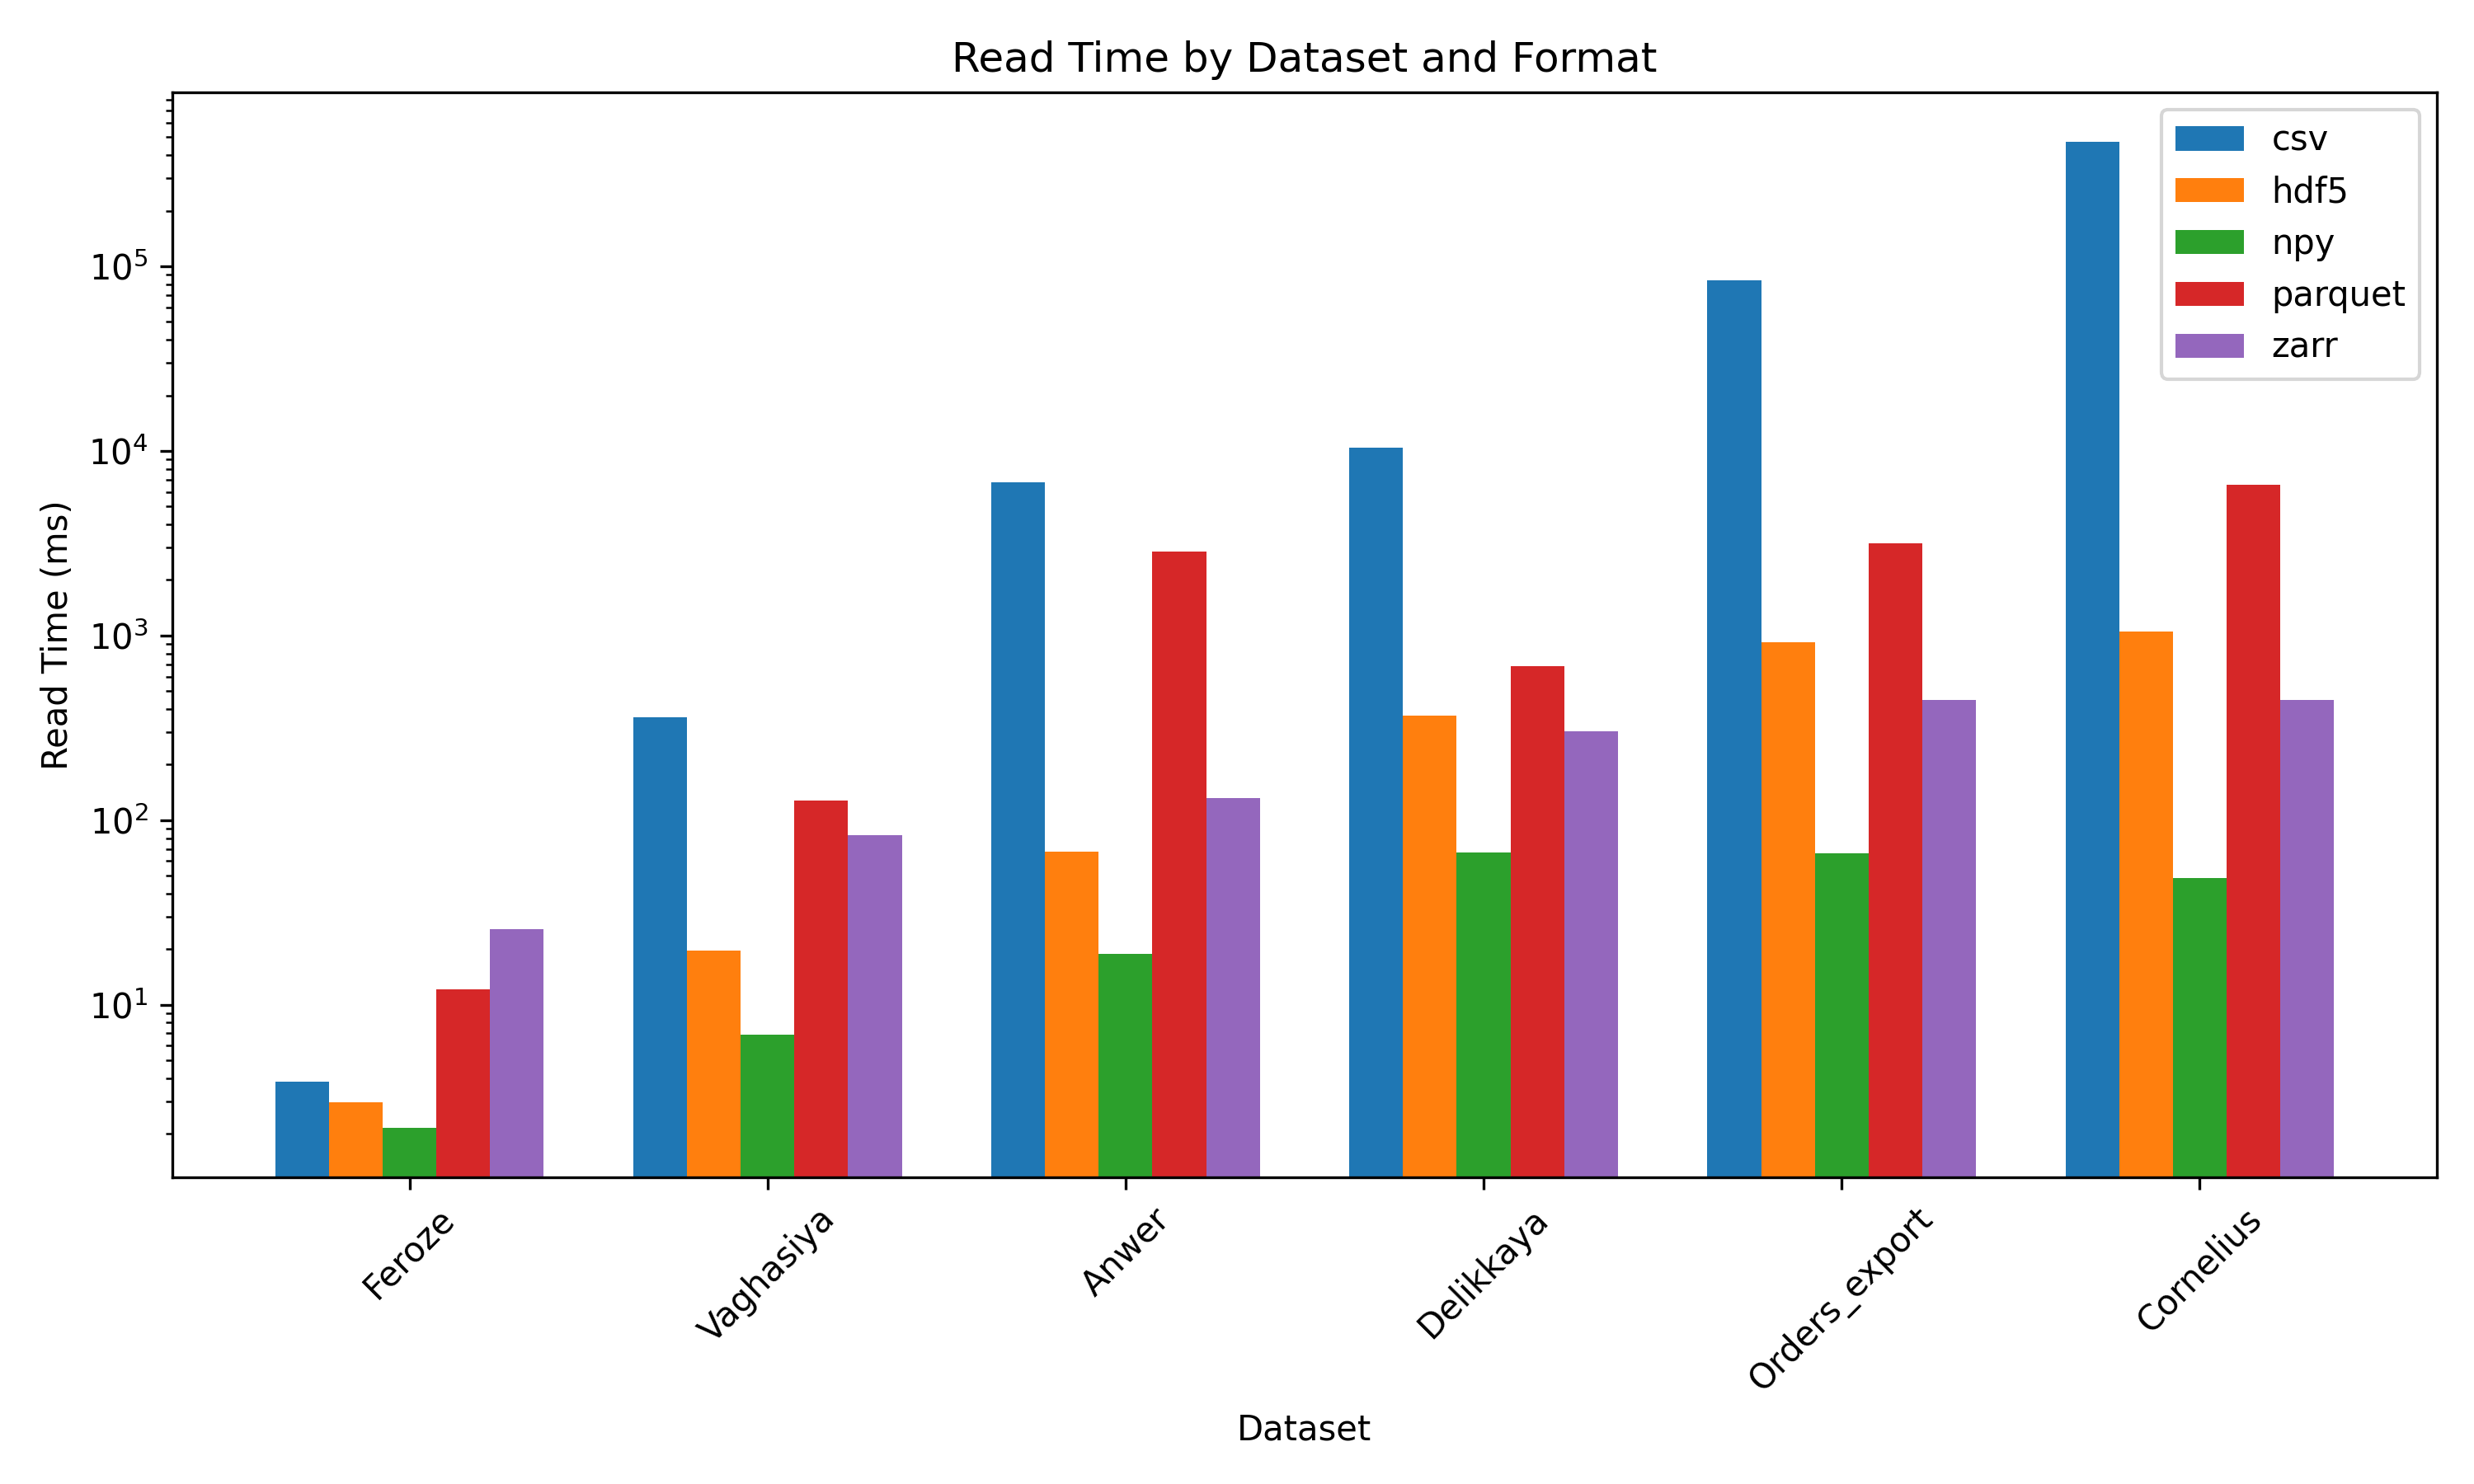
\includegraphics[width=0.9\columnwidth]{benchmark/read_time_by_dataset_and_format.png}
    \caption{Velocità di lettura dei formati di archiviazione delle matrici di raccomandazione}
    \label{fig:read-speed-recommendation-matrices}
\end{figure}

Si evince dunque che i dataset sono classificabili all'incirca così in ordine crescente di velocità di lettura:
\begin{enumerate}
    \item NPY;
    \item Zarr;
    \item HDF5;
    \item Parquet;
    \item CSV.
\end{enumerate}

Il grafico finale che mette assieme i risultati dei test di memoria occupata su disco e velocità di lettura è il seguente:

\begin{figure}[!h]
    \centering
    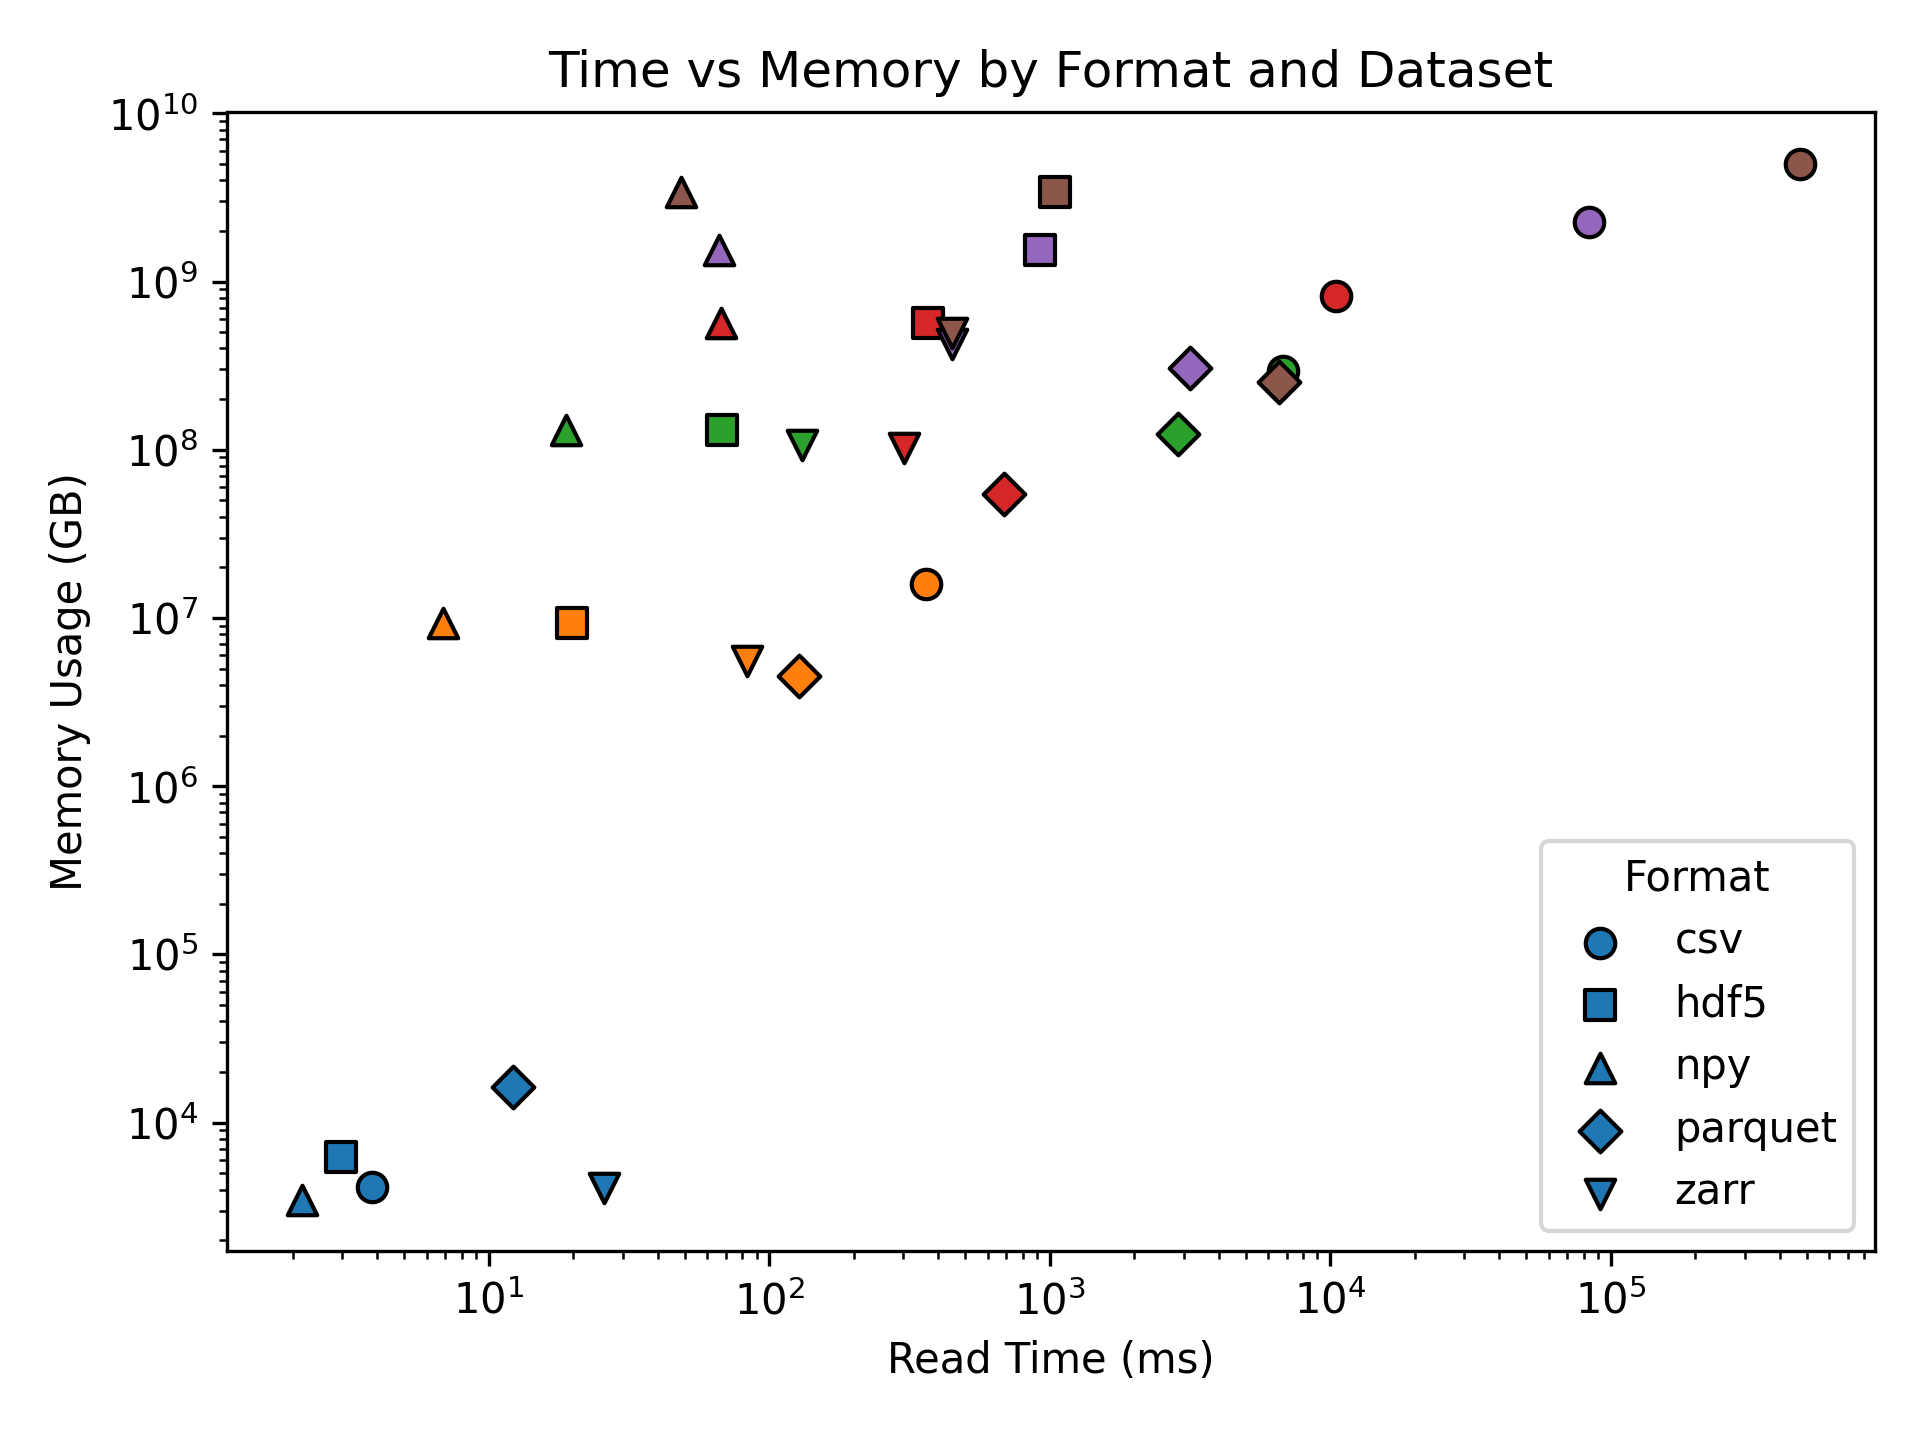
\includegraphics[width=0.9\columnwidth]{benchmark/time_vs_memory.png}
    \caption{Utilizzo della memoria e velocità di lettura dei formati di archiviazione delle matrici di raccomandazione}
    \label{fig:memory-usage-and-read-speed-recommendation-matrices}
\end{figure}

Mettendo i valori di memoria usata e velocità di lettura assieme, si evince che il formato Zarr è il migliore per le matrici di raccomandazione, poiché offre un buon compromesso tra spazio occupato su disco e velocità di lettura. Zarr è un formato progettato per la gestione di array multidimensionali e supporta la compressione e l'accesso parallelo ai dati, rendendolo adatto per l'archiviazione delle matrici. Inoltre, Zarr è ottimizzato per l'uso su cloud, il che lo rende compatibile con Google Cloud Storage, dove le matrici di raccomandazione saranno archiviate.

Dunque, si è deciso di utilizzare il formato Zarr per l'archiviazione delle matrici di raccomandazione, poiché offre un buon compromesso tra spazio occupato su disco e velocità di lettura, ed è compatibile con Google Cloud Storage.


\section{La predizione e rank fusion}

\section{Valutazione delle raccomandazioni}

\section{Collegamento con Google Cloud}

1) Spiegare situazione Oribea e cloud. Tasks e functions

\subsection{Google Cloud Functions}

1) Spiegare l'iniziale difficoltà dovuta al send\_file di cui non si era capita l'importanza
2) Spiegare l'obbligo di inviare uno zip, perchè sempre un file unico, altrimenti invia solo l'ultimo
3) Spiegare l'importanza della tanta RAM (32 GB invece di 256 MB)
4) Spiegare come è stato fondamentale mettere Python 3.13 perchè Zarr funzionasse
5) Configurazione di logging particolare per la stampa dei log

\subsection{Google Cloud Storage}

1) Introduzione: bisogno di tenere salvato materiale da una task all'altra
2) Spiegare come si è scelto di gestire i bucket
3) Spiegare come inizialmente si voleva identificare con il nome del csv, poi con la mail dell'utente. Poi si è capito che era tutto ambiguo, allora si è accettato di perdere family friendlieness e di mostrare un lungo token da copiare.
4) Spiegare differenza tra google.cloud.storage e gcsfs


\section{Frontend}
\label{sec:frontend}

Dopo aver caricato le due Functions di analisi delle vendite e di raccomandazione su Google Cloud Functions ed averle integrate nella piattaforma Oribea, si è deciso di provare a soddisfare anche il requisito desiderabile che prevede di sviluppare due interfacce grafiche per permettere agli utenti di interagire con le task in modo più semplice e intuitivo. Il reale obiettivo di queste interfacce è quello di garantire una validazione dell'input, assente nella piattaforma Oribea, in modo da evitare errori di contenuto nei file caricati oppure valori errati nei campi di testo, che potrebbero causare errori durante l'esecuzione delle task.

A causa delle difficoltà nello sviluppo di un backend che permetta l'integrazione con Google Cloud Functions, si è deciso di sviluppare due interfacce grafiche scollegate dalla logica funzionale, che possano essere dunque solamente un template personalizzabile che l'azienda Oribea potrà utilizzare per sviluppare le proprie interfacce grafiche in futuro.

Il contenuto effettivo di queste interfacce, data la natura delle tasks, è costituito unicamente da due form di input. Questo requisito ha dunque svolto una parte fondamentale nella scelta delle tecnologie da utilizzare per lo sviluppo.
Un altro requisito è stato quello che le interfacce fossero accessibili tramite un browser web, in modo da poter essere utilizzate da qualsiasi dispositivo connesso a Internet.

I framework di sviluppo web che sono stati presi in considerazione per lo sviluppo delle interfacce grafiche sono stati i seguenti:
\begin{itemize}
    \item \textbf{Angular}: Angular è un framework web completo sviluppato da Google, basato su TypeScript. Offre una struttura robusta e scalabile per lo sviluppo di applicazioni web complesse, con un'architettura basata su componenti, dependency injection integrato, e un ecosistema ricco di strumenti. È particolarmente adatto per progetti enterprise di grandi dimensioni;
    \item \textbf{React}: React è una libreria JavaScript sviluppata da Facebook per la costruzione di interfacce utente interattive. Si basa su un approccio dichiarativo e utilizza un DOM virtuale per ottimizzare le prestazioni. La sua architettura a componenti e la vasta community lo rendono ideale per progetti di varie dimensioni, dalle applicazioni semplici a quelle complesse;
    \item \textbf{Vue}: Vue è un framework JavaScript progressivo che combina la semplicità di utilizzo con la potenza necessaria per applicazioni complesse. Offre una curva di apprendimento graduale, un sistema di reattività intuitivo e una documentazione eccellente. È particolarmente apprezzato per la sua facilità d'uso e la capacità di integrarsi facilmente in progetti esistenti.
\end{itemize}

Data la grande semplicità delle interfacce grafiche da sviluppare, qualsiasi framework sarebbe stato in grado di soddisfare i requisiti. Allora, la differenza l'ha fatta il consiglio fornito da compagni di corso di laurea che avevano già avuto esperienza con questi framework, che hanno segnalati l'esistenza in React delle seguenti librerie dedicate ai form:
\begin{itemize}
    \item \textbf{React Hook Form}: è una libreria per la gestione efficiente dei form in React che si basa sull'utilizzo di hook. Offre prestazioni elevate minimizzando i re-render dei componenti, validazione integrata, e un'API semplice e intuitiva. È particolarmente apprezzata per la sua leggerezza e per la facilità di integrazione con librerie di validazione esterne;
    \item \textbf{Zod}: è una libreria di validazione schema-first per TypeScript e JavaScript che consente di definire schemi di validazione type-safe. Permette di validare dati in runtime garantendo al contempo la sicurezza dei tipi in fase di compilazione. È ideale per la validazione di form, API response e input utente;
    \item \textbf{Shadcn/ui}: è una collezione di componenti UI riutilizzabili costruiti con Radix UI e Tailwind CSS. Non è propriamente una libreria da installare, ma piuttosto un set di componenti che possono essere copiati e personalizzati direttamente nel progetto. Offre componenti moderni, accessibili e completamente customizzabili che seguono le migliori pratiche di design. In particolare, sono stati consigliati i componenti legati alla creazione di form, come i campi di input, i pulsanti e le etichette.
\end{itemize}

Dunque, grazie a questi consigli e alla semplicità delle interfacce grafiche da sviluppare, si è deciso di utilizzare React come framework di sviluppo, e di usufruire delle librerie React Hook Form, Zod e Shadcn/ui per la gestione dei form e la validazione degli input.

Successivamente, durante la progettazione delle interfacce, si è scelto, di comune accordo con il tutor, di adottare i seguenti approcci:
\begin{itemize}
    \item \textbf{Interfaccia di analisi delle vendite}: l'analisi del caso d'uso del servizio ha portato a progettare un'interfaccia ottimizzata per la visualizzazione a tutto schermo. Infatti, è stato pensato il servizio come standalone, e non come parte di un'applicazione più grande: un tecnico aziendale che deve analizzare le vendite archiviate in un dataset può così accedere al portale e concentrarsi esclusivamente sul fornire l'input al servizio;
    \item \textbf{Interfaccia di raccomandazione}: l'analisi del caso d'uso del servizio ha portato a progettare un'interfaccia ottimizzata per la visualizzazione su una finestrella di dimensioni ridotte. Infatti, è stato pensato il servizio come parte integrata di un'applicazione di e-commerce, che possa essere usata da un utente che sta navigando tra i prodotti e vuole ricevere delle raccomandazioni, oppure da un tecnico aziendale che, navigando tra gli stessi prodotti, vuole prevedere a quali utenti potrebbero interessare. In questo caso, l'interfaccia deve essere semplice, piccola e veloce da utilizzare, senza troppi fronzoli, in modo da non distrarre l'utente dalla navigazione.
\end{itemize}

Un altro aspetto affrontato durante lo sviluppo dell'interfaccia di analisi vendite è stata la scelta di integrare un'anteprima del file csv appena caricato, che ne mostrasse i nomi delle colonne e le prime righe, in modo da permettere all'utente di verificare che il file sia stato caricato correttamente e che contenga i dati attesi. Questa funzionalità è stata implementata utilizzando la libreria React Hook Form per la gestione del form di caricamento del file, e la libreria Papaparse per il parsing del file CSV e la visualizzazione dei dati in anteprima.

Un'anteprima del risultato finale delle interfacce grafiche sviluppate è mostrata nelle figure \ref{fig:frontend-sales-analysis} e \ref{fig:frontend-recommendation}.

\begin{figure}[!h]
    \centering
    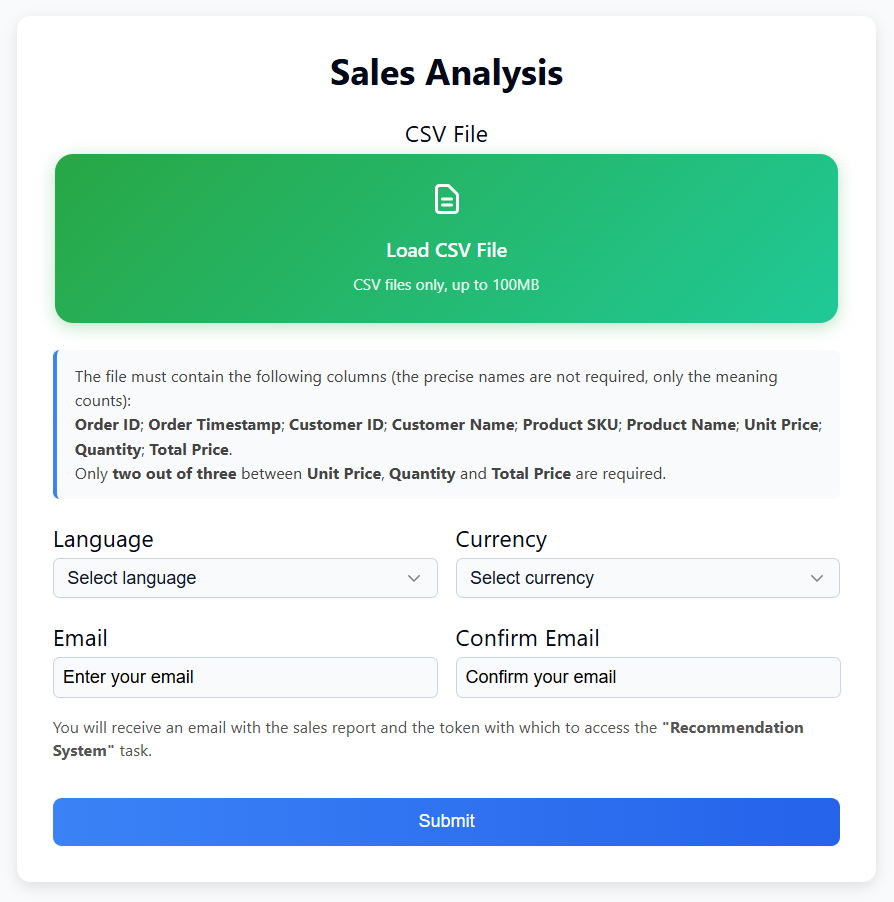
\includegraphics[width=0.8\columnwidth]{frontend/Frontend Sales Analysis.png}
    \caption{Interfaccia di analisi delle vendite}
    \label{fig:frontend-sales-analysis}
\end{figure}

\begin{figure}[!h]
    \centering
    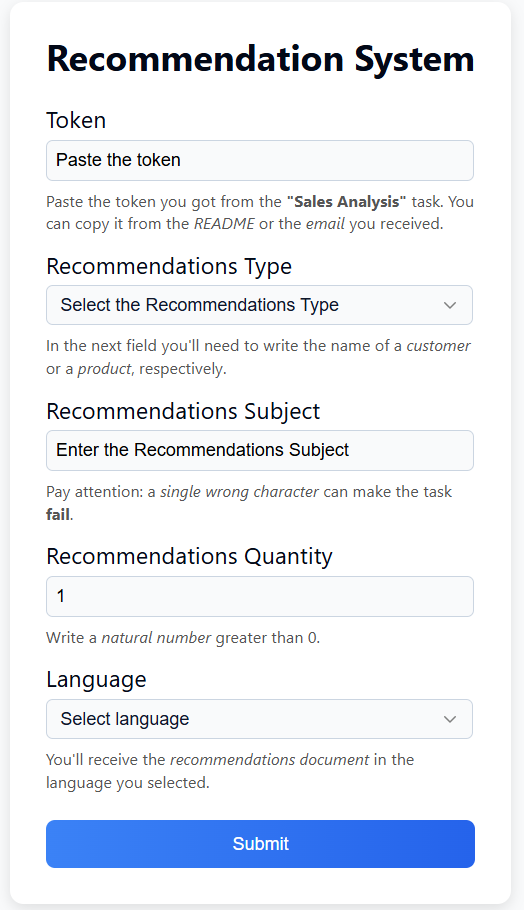
\includegraphics[width=0.3\columnwidth]{frontend/Frontend Recommendation.png}
    \caption{Interfaccia di raccomandazione}
    \label{fig:frontend-recommendation}
\end{figure}


\newpage

\subsection{Gestione dinamica del submit}

I submit dei due form delle interfacce grafiche sono stati gestiti in modo dinamico, in modo da poter gestire l'invio dei dati in modo diverso a seconda delle variabili d'ambiente configurate.

Inizialmente, prima ancora della scelta del framework di sviluppo, si era pensato di creare un'interfacce o classe astratta con la quale gestire il submit dei form, in modo da poter implementare più classi concrete che gestissero il submit in modo diverso a seconda dell'ambiente configurato. Tuttavia, dopo aver scelto React come framework di sviluppo, e considerato che React non possiede il concetto di classe, si è deciso di implementare il submit utilizzando gli hook: essi sono funzioni speciali di React che permettono di utilizzare lo stato e altre features all'interno di componenti funzionali, fornendo un'alternativa moderna e più flessibile rispetto ai componenti basati su classi.
La selezione dell'hook corretto da utilizzare è stata fatta tramite uno switch sul valore della variabile d'ambiente \texttt{VITE\_SUBMIT\_STRATEGY}, che può assumere i seguenti valori:
\begin{itemize}
    \item \texttt{api}: utilizza un hook personalizzato per inviare i dati del form tramite chiamata API;
    \item \texttt{log}: utilizza un hook che stampa i risultati del form su console.log;
    \item \texttt{alert}: utilizza un hook che mostra i risultati del form tramite un alert popup.
\end{itemize}

A supporto di questa configurazione, sono stati creati tre file di variabili d'ambiente nella root di entrambi i progetti:
\begin{itemize}
    \item \texttt{.env.development}: contiene le variabili d'ambiente dedicate allo sviluppo e al testing, e la strategia di submit è impostata su \texttt{alert};
    \item \texttt{.env.production}: contiene le variabili d'ambiente dedicate all'ambiente di produzione e all'integrazione con Google Cloud Functions, e la strategia di submit è impostata su \texttt{api};
    \item \texttt{.env.local}: contiene le variabili d'ambiente dedicate all'ambiente locale. Per quanto riguarda i due progetti sviluppati in questo stage, l'ambiente locale e l'ambiente di test sono stati equivalenti, ma è comuque una buona pratica separare un file di variabili d'ambiente locali per eventuali differenziazioni future. A causa dell'attuale equivalenza tra ambiente locale e ambiente di test, questo file contiene le stesse variabili del file \texttt{.env.development}, e quindi la strategia di submit è impostata su \texttt{alert}.
\end{itemize}

Dunque, a seconda della variabile d'ambiente \texttt{VITE\_SUBMIT\_STRATEGY} configurata, il submit dei form delle interfacce grafiche invierà i dati in modo diverso, permettendo di testare i form, in particolare la validazione sviluppata con \texttt{Zod}, senza dover necessariamente inviare i dati a Google Cloud Functions o ad un server esterno.

Attualmente, il submit non è ancora stato integrato con Google Cloud Functions, poiché si è deciso di sviluppare le interfacce grafiche come template personalizzabili, e quindi non sono state implementate le chiamate \gls{api} per l'invio dei dati. Tuttavia, la struttura del codice è già pronta per essere integrata con le \gls{api} di Google Cloud Functions in futuro, semplicemente modificando la variabile d'ambiente \texttt{VITE\_SUBMIT\_STRATEGY} in "\texttt{api}" e aggiornando l'apposito \texttt{hook}.



\section{Ottimizzazione}

L'ultima attività svolta durante lo sviluppo della task di analisi delle vendite è stata l'ottimizzazione del codice, in modo da migliorare le prestazioni e ridurre i tempi di esecuzione. In particolare, sono state implementate le seguenti migliorie:

\begin{itemize}
    \item \textbf{Introduzione delle Pandas Vectorized Ops}: per migliorare le prestazioni delle operazioni sui dataframe, sono state utilizzate le Pandas Vectorized Ops, che consentono di eseguire operazioni su interi array di dati in modo più efficiente rispetto alle operazioni iterabili, come ad esempio un ciclo for. Questo ha portato a un notevole miglioramento delle prestazioni durante il preprocessing dei dati, il calcolo delle statistiche e la generazione dei grafici;
    \item \textbf{Eliminazione delle operazioni apply}: sono state eliminate le operazioni apply, che sono meno efficienti rispetto alle operazioni vettorializzate, e sono state sostituite appunto con queste ultime. Questo ha portato ad un ulteriore miglioramento delle prestazioni nel calcolo delle statistiche e ad un efficientamento nella formattazione delle date e dei prezzi;
    \item \textbf{Miglioramento dell'algoritmo delle etichette}: l'algoritmo per la disambiguazione dei prodotti con lo stesso nome utilizzando etichette ("(1), (2), ..."), utilizzato per il grafico dei top 5 prodotti per fatturato, è stato migliorato in modo da essere più efficiente e veloce. In particolare, è stata creata una funzione dedicata (\texttt{create\_unique\_product\_names}), che utilizza un approccio a due fasi: prima calcola la frequenza di ciascun nome prodotto utilizzando \texttt{value\_counts()}, poi itera una sola volta sui nomi mantenendo un contatore per i duplicati e aggiungendo il suffisso numerico solo ai nomi che compaiono più volte. Questo approccio evita iterazioni multiple e controlli ridondanti, portando a un notevole miglioramento delle prestazioni durante la generazione del grafico.
\end{itemize}

Dopo aver svolto queste ottimizzazioni, sono stati eseguiti dei test di performance per verificare i miglioramenti ottenuti: è stato cioè misurato il tempo di esecuzione della task di analisi vendite prima e dopo l'ottimizzazione. Per ottenere la versione della cloud function non ancora ottimizzata è stato fatto uso del comando \texttt{git switch}, che ha permesso di tornare all'ultimo commit prima dell'ottimizzazione, e sono stati eseguiti i test di performance su quella versione. Poi, è bastato rieseguire \texttt{git switch} verso il commit più recente per fare i test sulla versione ottimizzata. I test cronometrati sono stati eseguiti su tutti i dieci dataset disponibili.
I risultati dei test sono mostrati nella seguente tabella (\ref{tab:performance-tests}).

\begin{table}[h]
    \centering
    \begin{tabular}{|l|c|c|c|}
        \hline
        \textbf{Dataset} & \textbf{Tempo pre-otti} & \textbf{Tempo post-otti} & \textbf{Miglioramento (\%)} \\
        \hline
        Swillm & 01:50 & 01:08 & 38,2\% \\
        Dee & 00:58 & 00:38 & 34,5\% \\
        Anwer & 03:01 & 02:00 & 33,7\% \\
        Orders\_export & 03:40 & 02:48 & 23,6\% \\
        Cornelius & 05:21 & 04:34 & 14,6\% \\
        Vaghasiya & 00:53 & 00:49 & 7,5\% \\
        Segura & 00:50 & 00:47 & 6,0\% \\
        Shaw & 00:55 & 00:53 & 3,6\% \\
        Feroze & 00:40 & 00:39 & 2,5\% \\
        Delikkaya & 02:02 & 02:07 & -4,1\% \\
        \hline
    \end{tabular}
    \caption{Risultati dei test di performance prima e dopo l'ottimizzazione}
    \label{tab:performance-tests}
\end{table}

\newpage

Dall'analisi di questi risultati, si distinguono tre fasce di variazione del tempo di esecuzione:
\begin{itemize}
    \item \textbf{Miglioramento elevato}: i dataset Swillm, Dee e Anwer hanno mostrato un miglioramento significativo, con una riduzione del tempo di esecuzione superiore al 30\%. Questo indica che le ottimizzazioni hanno avuto un impatto notevole su dataset di dimensioni maggiori o con una struttura più complessa;
    \item \textbf{Miglioramento moderato}: i dataset Orders\_export, Cornelius, Vaghasiya, Segura e Shaw hanno mostrato un miglioramento compreso tra il 6\% e il 23\%. Questi risultati suggeriscono che le ottimizzazioni hanno avuto un effetto positivo, ma non così marcato come nei casi precedenti;
    \item \textbf{Miglioramento minimo o negativo}: i dataset Feroze e Delikkaya hanno mostrato un miglioramento minimo (2,5\%) o addirittura un peggioramento (-4,1\%). Questo potrebbe essere dovuto alla natura specifica di questi dataset o alla presenza di operazioni che non sono state significativamente influenzate dalle ottimizzazioni.
\end{itemize}

In generale, le ottimizzazioni hanno portato a un miglioramento significativo delle prestazioni della task di analisi delle vendite, con una riduzione media del tempo di esecuzione superiore al 20\%. Tuttavia, è importante notare che i risultati possono variare a seconda della natura specifica dei dataset e delle operazioni svolte su di essi.

Il requisito di ottimizzazione è stato dunque soddisfatto, e le prestazioni della task sono state notevolmente migliorate, rendendo il sistema più efficiente e veloce nell'elaborazione dei dati delle vendite.
 % Progettazione e Implementazione, non consigliato da Zanella ma lo metto lo stesso
    \chapter{Verifica e validazione}
\label{cap:verifica-validazione}

\intro{Breve introduzione al capitolo}\\

\section{Scelte riguardanti i test}

\section{Test di unità}

\section{Test dell’LLM}
 % Verifica e Validazione, non consigliato da Zanella ma lo metto lo stesso
    \chapter{Conclusioni}
\label{cap:conclusioni}

\intro{In questo capitolo, vengono presentate le conclusioni del progetto, con un riepilogo degli obiettivi raggiunti, delle conoscenze acquisite e dei possibili miglioramenti futuri. Si conclude con una valutazione personale dell'esperienza di sviluppo.}


\section{Considerazioni finali}

Il periodo di tirocinio del laureando Stefani Riccardo ha avuto l'obiettivo di sviluppare un sistema di analisi vendite ed un sistema di raccomandazione per un'azienda di e-commerce, con l'intento di migliorare l'esperienza utente e incrementare le vendite attraverso suggerimenti personalizzati. Il progetto ha richiesto l'analisi dei dati di vendita esistenti, la preparazione dei dati, lo sviluppo di algoritmi di raccomandazione e l'integrazione con l'infrastruttura aziendale. L'implementazione è stata realizzata utilizzando tecnologie moderne come Python, machine learning e integrazione con \gls{googlecloudplatform}.

La maggior parte del tempo è stata dedicata all'analisi e preparazione dei dati di vendita, fase cruciale per garantire l'efficacia del sistema di raccomandazione. Il sistema sviluppato si è rivelato utile per l'azienda, fornendo sia informazioni sui trend di vendita utili per le decisioni strategiche, sia raccomandazioni personalizzate per gli utenti. Questo ha permesso di migliorare l'esperienza di acquisto, aumentando la soddisfazione del cliente e le vendite complessive.

Il sistema è stato implementato in due tasks caricate nella piattaforma Oribea, una per l'analisi delle vendite e l'altra per il sistema di raccomandazione. Sono state inoltre fornite due corrispettive interfacce utente contenenti i form che permettono di accedere alle due funzionalità senza passare attraverso la piattaforma aziendale. Il sistema è stato testato con successo su 10 dataset di vendita reali, dimostrando la sua efficacia e utilità.

È importante sottolineare, tuttavia, che il funzionamento del sistema è strettamente legato alla qualità e completezza del dataset fornito, che infatti deve possedere esattamente le colonne richieste per l'analisi delle vendite e deve possedere un numero sufficiente interazioni cliente-prodotto per generare raccomandazioni significative. Senza le colonne corrette, il sistema restituisce un errore e non può essere utilizzato. Inoltre, se il dataset è troppo scarso, le raccomandazioni generate potrebbero non essere utili o addirittura fuorvianti.


\section{Raggiungimento degli obiettivi}

Tutti i requisiti funzionali e non funzionali identificati nell'analisi iniziale e riportati nel capitolo \S\ref{cap:analisi-requisiti} sono stati raggiunti con successo.

Tra gli obiettivi definiti nel \emph{Piano di Lavoro} e riportati alla sezione \S\ref{sec:obiettivi-stage}, l'unico obiettivo non soddisfatto è stato l'obiettivo opzionale OZ1 relativo all'implementazione di un chatbot che si potesse collegare ad entrambe le \gls{cloudfunctions} e potesse così fornire entrambi i servizi in modo conversazionale, che si è rivelato troppo complesso da realizzare nei tempi disponibili nel tirocinio.


\section{Conoscenze acquisite}

Il tirocinio svolto ha soddisfatto appieno le aspettative: nonostante il progetto sia risultato piuttosto impegnativo, è stato molto utile per approfondire diverse tecnologie ed algoritmi, per acquisire competenze nell’ambito dei sistemi di analisi dati e di raccomandazione e per sperimentare alcune reali applicazioni di strumenti di intelligenza artificiale.

In particolare, le principali nuove conoscenze e competenze maturate durante il
periodo di stage sono le seguenti:

\begin{itemize}
    \item Approfondimento del linguaggio di programmazione Python e delle sue librerie per data science;
    \item Competenze nella preparazione e analisi di grandi volumi di dati;
    \item Competenze nella stesura di analisi delle vendite e reportistica;
    \item Competenze nello sviluppo di sistemi di raccomandazione nell'ambito e-commerce;
    \item Competenze nel collegamento e utilizzo di Google Cloud Platform;
    \item Competenze nell'integrazione con software aziendali pre-esistenti;
    \item Competenze nello sviluppo frontend di interfacce utente;
    \item Competenze di ottimizzazione delle performance di sistemi di analisi dati;
    \item Competenze nella stesura della documentazione tecnica di progetti software.
\end{itemize}


\section{Possibili miglioramenti futuri}

Nonostante il successo generale del sistema sviluppato, alcune funzionalità interessanti non sono state implementate per questioni di tempo e complessità. I possibili miglioramenti futuri includono:

\begin{itemize}
    \item Implementazione di un chatbot che possa interagire con gli utenti e fornire raccomandazioni personalizzate in modo conversazionale, e possa altrettanto comunicare l'analisi delle vendite ai proprietari dell'e-commerce, integrando così le due tasks sviluppate;
    \item Implementazione di un sistema di logging avanzato per monitorare l'esecuzione e le performance delle due tasks;
    \item Implementazione di algoritmi più sofisticati per migliorare la serendipità delle raccomandazioni;
    \item Implementazione di tecniche di \gls{data-reduction} per ridurre la dimensione delle matrici di raccomandazione senza compromettere la qualità dei risultati.
\end{itemize}

\section{Valutazione personale}

Questo progetto di tirocinio ha rappresentato un'importante tappa nel completamento del percorso universitario, permettendo di mettere in pratica le conoscenze teoriche acquisite, in particolare nell'ambito dell'Ingegneria del Software e dell'analisi dati.

L'esperienza è stata particolarmente utile per la crescita professionale a livello tecnico, fornendo competenze pratiche direttamente applicabili nel mondo del lavoro. Tuttavia, lavorando principalmente da remoto e in autonomia, non è stato purtroppo possibile sviluppare competenze di lavoro di squadra o di dinamiche aziendali.

Nonostante questa limitazione, sono complessivamente soddisfatto del risultato finale: gli obiettivi prefissati sono stati raggiunti e le competenze acquisite costituiscono una solida base per il proseguimento degli studi con la laurea magistrale e per future opportunità professionali nel campo dell'informatica e dell'analisi dati.


    % \appendix
    % \chapter{Appendice A}

\epigraph{Citazione}{Autore della citazione}
 % Nessun tesista recente ha scritto appendici, quindi non le metto

    \backmatter
    \printglossary[type=\acronymtype, title=Acronimi e abbreviazioni, toctitle=Acronimi e abbreviazioni]
    \printglossary[type=main, title=Glossario, toctitle=Glossario]

    \cleardoublepage
\chapter{Bibliografia}

\nocite{*}

% Print book bibliography
%\printbibliography[heading=subbibliography,title={Libri},type=book,resetnumbers=true]
\printbibliography[heading=subbibliography,title={Libri},category=libri,resetnumbers=true]

% Print article bibliography
%\printbibliography[heading=subbibliography,title={Riferimenti bibliografici},type=book,resetnumbers=true]
\printbibliography[heading=subbibliography,title={Articoli},category=articoli,resetnumbers=true]

% Print site bibliography
%\printbibliography[heading=subbibliography,title={Siti web consultati},type=online,resetnumbers=true]
\printbibliography[heading=subbibliography,title={Siti web},category=web,resetnumbers=true]

\end{document}
